\documentclass[a4paper]{report}

% --- FONT & NGÔN NGỮ ---
\usepackage{fontspec}
\setmainfont{Times New Roman}
\usepackage[vietnamese]{babel}
\usepackage{microtype} % Tự động tinh chỉnh khoảng cách để giảm lỗi tràn lề

% --- ÉP FONT 13pt TOÀN CỤC ---
\usepackage{fontsize}
\changefontsize[15.6]{13} % Cỡ chữ 13pt, base leading 15.6pt

% --- CANH LỀ CHUẨN A4 KHÓA LUẬN TỐT NGHIỆP TDTU ---
% Lề trái 3.5cm (đóng gáy sách), lề phải 2.0cm, lề trên 3.0cm, lề dưới 3.0cm
\usepackage[top=3.0cm, bottom=3.0cm, left=3.5cm, right=2.0cm, headheight=16pt, headsep=1.0cm, footskip=1.2cm]{geometry}

% --- DÃN DÒNG & THỤT ĐẦU DÒNG ĐOẠN VĂN ---
\usepackage{setspace}
\onehalfspacing % Dãn dòng 1.5 lines chuẩn
\usepackage{indentfirst}
\setlength{\parindent}{1.27cm} % Thụt đầu dòng 1.27cm (0.5 inch)
\setlength{\parskip}{0pt}      % Không dãn cách đoạn thừa thãi
\emergencystretch 3em          % Chống tuyệt đối lỗi tràn lề phải (overfull hbox)

% --- HEADER & FOOTER: ĐÁNH SỐ TRANG GIỮA TRÊN ---
\usepackage{fancyhdr}
\pagestyle{fancy}
\fancyhf{} 
\fancyhead[C]{\fontsize{10pt}{12pt}\selectfont\thepage} % Số trang căn giữa phía trên
\renewcommand{\headrulewidth}{0pt}
\renewcommand{\footrulewidth}{0pt}

% Đảm bảo trang đầu chương / trang plain vẫn có số trang căn giữa phía trên
\fancypagestyle{plain}{
    \fancyhf{} 
    \fancyhead[C]{\fontsize{10pt}{12pt}\selectfont\thepage} 
    \renewcommand{\headrulewidth}{0pt}
}

% --- TOÁN HỌC & HÌNH ẢNH ---
\usepackage{amsmath, amsfonts, amssymb}
\usepackage{graphicx}
\usepackage{tikz}
\usetikzlibrary{calc, arrows.meta, positioning, fit, backgrounds}
% --- SƠ ĐỒ: bảng màu và biểu tượng dùng chung (tồn kho đa kho) ---
\usetikzlibrary{shapes.geometric, decorations.pathreplacing, shadows}
\definecolor{khoNavy}{HTML}{1F3A5F}
\definecolor{khoCam}{HTML}{E07B24}
\definecolor{khoXanh}{HTML}{2A9D8F}
\definecolor{khoDo}{HTML}{C0392B}
\definecolor{khoNen}{HTML}{F3F5F8}
\tikzset{
    % Cỡ chữ cố định trong sơ đồ, không phụ thuộc cỡ chữ 13pt của thân bài
    soDo/.style={execute at begin picture={%
        \renewcommand\small{\fontsize{10.95}{13.6}\selectfont}%
        \renewcommand\footnotesize{\fontsize{10}{12}\selectfont}%
        \renewcommand\scriptsize{\fontsize{8}{9.5}\selectfont}%
        \renewcommand\tiny{\fontsize{6}{7}\selectfont}}},
    khung/.style={draw=khoNavy!60, fill=khoNen, rounded corners=3pt, line width=0.6pt,
                  align=center, font=\small, inner sep=4pt},
    khungTacTu/.style={khung, draw=khoXanh, fill=khoXanh!10},
    khungDam/.style={khung, draw=khoNavy, fill=khoNavy, text=white},
    khungChiPhi/.style={khung, draw=khoDo!70, fill=khoDo!7},
    nhan/.style={font=\footnotesize, text=khoNavy, align=center},
    muiTen/.style={-{Stealth[length=2.6mm, width=2mm]}, line width=0.9pt, draw=khoNavy},
    muiCam/.style={muiTen, draw=khoCam},
    muiXanh/.style={muiTen, draw=khoXanh},
    muiDo/.style={muiTen, draw=khoDo},
    % Nhà kho: #1 = mức đầy (0..1) của thanh sức chứa
    pics/kho/.style={code={
        \fill[khoNavy!12] (-0.9,0) rectangle (0.9,0.95);
        \draw[khoNavy, line width=0.8pt] (-0.9,0) -- (-0.9,0.95) -- (0,1.45) -- (0.9,0.95) -- (0.9,0) -- cycle;
        \fill[khoNavy!45] (-0.3,0) rectangle (0.3,0.6);
        \foreach \x in {-0.3,-0.1,0.1} \draw[khoNavy!70, line width=0.3pt] (\x+0.1,0) -- (\x+0.1,0.6);
        \foreach \x/\y in {-0.75/0, -0.75/0.22, 0.45/0, 0.45/0.22}
            \filldraw[fill=khoCam!70, draw=khoCam!90!black, line width=0.3pt] (\x,\y) rectangle ++(0.26,0.2);
        \draw[khoNavy, line width=0.5pt] (1.05,0) rectangle (1.25,1.2);
        \fill[khoCam] (1.05,0) rectangle (1.25,{1.2*#1});
    }},
    % Xe tải giao hàng
    pics/xe/.style={code={
        \filldraw[fill=khoCam!80, draw=khoCam!70!black, line width=0.5pt, rounded corners=1pt] (-0.9,0.15) rectangle (0.3,0.85);
        \filldraw[fill=khoNavy!80, draw=khoNavy, line width=0.5pt, rounded corners=1.5pt] (0.32,0.15) -- (0.32,0.65) -- (0.6,0.65) -- (0.85,0.4) -- (0.85,0.15) -- cycle;
        \fill[white!85!khoNavy] (0.4,0.42) rectangle (0.58,0.6);
        \foreach \x in {-0.6,0.55} \filldraw[fill=khoNavy, draw=white, line width=0.5pt] (\x,0.13) circle (0.13);
    }},
    % Khách hàng
    pics/khach/.style={code={
        \foreach \x/\c in {-0.35/khoNavy!55, 0.35/khoNavy!55, 0/khoNavy} {
            \fill[\c] (\x,0.78) circle (0.17);
            \fill[\c] (\x-0.27,0.05) .. controls (\x-0.27,0.55) and (\x+0.27,0.55) .. (\x+0.27,0.05) -- cycle;
        }
    }},
}
\usepackage{float}
\usepackage{placeins}  % \FloatBarrier: giữ bảng, hình của chương trước mục tóm tắt
% Trang chỉ chứa bảng/hình: đặt từ đầu trang thay vì căn giữa theo chiều dọc (tránh khoảng trắng lớn phía trên).
\makeatletter
\setlength{\@fptop}{0pt}
\setlength{\@fpbot}{0pt plus 1fil}
\setlength{\@fpsep}{\floatsep}
\makeatother
% Cho bảng, hình nằm chung trang với chữ nhiều hơn: ít trang chỉ có float, ít khoảng trắng cuối trang.
\renewcommand{\topfraction}{0.9}
\renewcommand{\bottomfraction}{0.8}
\renewcommand{\textfraction}{0.1}
\renewcommand{\floatpagefraction}{0.8}
\usepackage{longtable}
\usepackage{booktabs}
\usepackage{array}
\usepackage{multirow}
\usepackage{tabularx}
\usepackage{xltabular}
\newcolumntype{Y}{>{\centering\arraybackslash}X}
% Bảng kẻ lưới đầy đủ (| và \hline): thêm khoảng đệm trên mỗi hàng để chữ không sát đường kẻ.
\setlength{\extrarowheight}{2pt}
% Ô hai dòng: \tbl, \tbr, \tbc{dòng 1}{dòng 2} căn trái, phải, giữa (tiêu đề cột dài, không phải co bảng).
\newcommand{\tbl}[2]{\begin{tabular}[c]{@{}l@{}}#1\\#2\end{tabular}}
\newcommand{\tbr}[2]{\begin{tabular}[c]{@{}r@{}}#1\\#2\end{tabular}}
\newcommand{\tbc}[2]{\begin{tabular}[c]{@{}c@{}}#1\\#2\end{tabular}}
% \ghichu{...}: ghi chú ngắn dưới bảng (ký hiệu, đơn vị); chú thích bảng chỉ giữ cụm danh từ ngắn.
\newcommand{\ghichu}[1]{\par\smallskip\begin{minipage}{\linewidth}\small\textit{Ghi chú:} #1\end{minipage}}
\usepackage{subcaption}
\graphicspath{{media/}}
\usepackage{caption}
\captionsetup{
    font={small},
    labelfont={bf},
    labelsep=colon,
    skip=6pt
}

\usepackage[hidelinks]{hyperref} % Liên kết mục lục sạch sẽ, không viền đỏ

% --- TÙY CHỈNH MỤC LỤC & DANH MỤC (TOC, LOF, LOT) ---
\usepackage{tocloft} 
\renewcommand{\cftdotsep}{0.5} % Dấu chấm mục lục san sát chuẩn Word

% Thêm chữ "CHƯƠNG " vào Mục lục
\renewcommand{\cftchappresnum}{CHƯƠNG } 
\renewcommand{\cftchapaftersnum}{. }    
\setlength{\cftchapnumwidth}{6.0em}     

% 1. Cấp Chương (Chapter): In đậm toàn hàng
\renewcommand{\cftchapfont}{\bfseries}
\renewcommand{\cftchapleader}{\bfseries\cftdotfill{\cftdotsep}}
\renewcommand{\cftchappagefont}{\bfseries}

\setlength{\cftchapindent}{0pt}

% 2. Cấp Mục (Section - 1.1): Chữ thường, thụt 0.635cm
\renewcommand{\cftsecfont}{\normalfont}
\renewcommand{\cftsecleader}{\normalfont\cftdotfill{\cftdotsep}}
\renewcommand{\cftsecpagefont}{\normalfont}
\setlength{\cftsecindent}{0.635cm}
\setlength{\cftsecnumwidth}{2.2em}

% 3. Cấp Tiểu mục (Subsection - 1.1.1): In nghiêng, thụt 1.27cm
\renewcommand{\cftsubsecfont}{\itshape}
\renewcommand{\cftsubsecleader}{\itshape\cftdotfill{\cftdotsep}}
\renewcommand{\cftsubsecpagefont}{\itshape}
\setlength{\cftsubsecindent}{1.27cm}
\setlength{\cftsubsecnumwidth}{2.8em}

% Dòng đầu của mục, tiểu mục bị mất phần thụt (\parindent của mục lục về 0), nên chèn lại bằng tay.
% Dòng ngắt xuống vẫn thụt theo \leftskip = indent + numwidth nên thẳng hàng với chữ tiêu đề.
\renewcommand{\cftsecfont}{\normalfont\hspace*{\cftsecindent}}
\renewcommand{\cftsubsecfont}{\itshape\hspace*{\cftsubsecindent}}
% Lề phải: số trang rộng 2em, tiêu đề dừng cách lề 3,5em để luôn còn dấu chấm dẫn trước số trang.
\cftsetpnumwidth{2em}
\cftsetrmarg{3.5em}

% Khoảng cách giữa các dòng trong Mục lục
\setlength{\cftbeforechapskip}{8pt} 
\setlength{\cftbeforesecskip}{5pt}
\setlength{\cftbeforesubsecskip}{4pt}

% Danh mục hình vẽ
\renewcommand{\cftfigpresnum}{Hình } 
\renewcommand{\cftfigaftersnum}{: }  
\setlength{\cftfignumwidth}{5.3em}   % đủ cho "Hình 4.10: "

% Danh mục bảng biểu
\renewcommand{\cfttabpresnum}{Bảng }
\renewcommand{\cfttabaftersnum}{: }
\setlength{\cfttabnumwidth}{5.3em}   % đủ cho "Bảng 4.10: "

% Xóa khoảng trắng thừa giữa các chương trong danh mục hình/bảng
\usepackage{etoolbox}
\makeatletter
\AtBeginDocument{
  \patchcmd{\@chapter}{\addtocontents{lof}{\protect\addvspace{10\p@}}}{}{}{}
  \patchcmd{\@chapter}{\addtocontents{lot}{\protect\addvspace{10\p@}}}{}{}{}
}
\makeatother

% --- ĐỊNH DẠNG TIÊU ĐỀ CÁC CẤP (HEADING SPACING CHUẨN ĐẸP) ---
\usepackage{titlesec}
\setcounter{secnumdepth}{3} % Đánh số tới cấp 1.1.1.1

% Heading 1: Chương (\chapter) - 16pt Bold
\titleformat{\chapter}[hang]
  {\fontsize{16pt}{22pt}\selectfont\bfseries} 
  {CHƯƠNG \thechapter.} 
  {0.5cm} 
  {}
\titlespacing*{\chapter}{0pt}{0pt}{16pt} % Cách dưới 16pt

% Heading 2: Mục lớn (\section) - 14pt Bold, sát lề trái 0cm
\titleformat{\section}[hang]
  {\fontsize{14pt}{19pt}\selectfont\bfseries} 
  {\thesection}
  {0.4cm} 
  {}
\titlespacing*{\section}{0pt}{14pt}{6pt} % Sát lề trái

% Heading 3: Tiểu mục (\subsection - vd 3.1.1) - 13pt Bold Italic, thụt vào 0.635cm (nửa tab)
\titleformat{\subsection}[hang]
  {\fontsize{13pt}{18pt}\selectfont\bfseries\itshape} 
  {\thesubsection}
  {0.35cm} 
  {}
\titlespacing*{\subsection}{0.635cm}{10pt}{4pt} % Thụt vào bậc thang 0.635cm

% Heading 4: Tiểu mục con (\subsubsection - vd 3.1.1.1) - 13pt Italic, thụt vào 1.27cm (1 tab)
\titleformat{\subsubsection}[hang]
  {\fontsize{13pt}{18pt}\selectfont\itshape} 
  {\thesubsubsection}
  {0.3cm} 
  {}
\titlespacing*{\subsubsection}{1.27cm}{8pt}{3pt} % Thụt vào bậc thang 1.27cm

% --- KHOẢNG CÁCH CÔNG THỨC TOÁN HỌC ---
\AtBeginDocument{
  \setlength{\abovedisplayskip}{6pt}
  \setlength{\belowdisplayskip}{6pt}
  \setlength{\abovedisplayshortskip}{3pt} 
  \setlength{\belowdisplayshortskip}{3pt}
}

% --- TÀI LIỆU THAM KHẢO ---
\usepackage{csquotes} 
\DeclareQuoteAlias{english}{vietnamese}

\usepackage[backend=biber, style=ieee, language=english, autolang=none, defernumbers=true]{biblatex}
% Tài liệu tham khảo chia theo chủ đề (main.tex in từng nhóm); defernumbers: đánh số liên tục theo thứ tự in.
% Thêm nguồn mới vào references.bib thì phải gán nó vào một nhóm dưới đây, nếu không nguồn đó không được in.
\DeclareBibliographyCategory{tonkho}\addtocategory{tonkho}{harris1913,arrow1951,scarf1960,clark1960,zipkin2000,zipkin2008,silver2016,lee1997}
\DeclareBibliographyCategory{rl}\addtocategory{rl}{bellman1957,puterman1994,sutton2018,schulman2015trpo,schulman2016gae,schulman2017ppo,ng1999,stooke2020,altman1999}
\DeclareBibliographyCategory{marl}\addtocategory{marl}{bernstein2002,oliehoek2016,tan1993,gupta2017,dewitt2020ippo,yu2022mappo,wolpert2001,devlin2011potential,christianos2021seps,zaheer2017deepsets}
\DeclareBibliographyCategory{rltonkho}\addtocategory{rltonkho}{oroojlooyjadid2022,gijsbrechts2022,yang2023mabim,ding2022cdppo,liu2025happo,kotecha2024decentralized,demoor2022reward,zhu2026spatiotemporal,jeong2026alca,boute2022,kaynov2024,vanvuchelen2020,maggiar2025,madeka2022}
\DeclareBibliographyCategory{dubao}\addtocategory{dubao}{ke2017lightgbm,croston1972,syntetos2005accuracy,syntetos2005categorization,kostenko2006,makridakis2022background,makridakis2022accuracy,m5dataset,banrudin2019,elmachtoub2022}
\DeclareBibliographyCategory{danhgia}\addtocategory{danhgia}{brockman2016gym,towers2024gymnasium,hubbs2020orgym,henderson2018,agarwal2021,kunsch1989}
% biblatex khong co vietnamese.lbx -> cac chuoi (vol., no., et al., in Proc.)
% bi in thang ten khoa noi bo (jourvol, andothers). Dung chuoi tieng Anh
% cho danh muc tai lieu, dung quy uoc IEEE.
\DeclareLanguageMapping{vietnamese}{english}
\DefineBibliographyStrings{vietnamese}{%
  url     = {\mkbibbrackets{Online}\adddot\space Available},
  urlseen = {Accessed},
}
\addbibresource{backmatter/references.bib}
\usepackage{xurl}
% Cho phép ngắt DOI/URL sau chữ số và chữ hoa để DOI dài không tràn lề phải.
\setcounter{biburlnumpenalty}{100}
\setcounter{biburlucpenalty}{100}
\let\parencite\cite



\defbibheading{bibcenter}{
    \clearpage
    \phantomsection
    \addcontentsline{toc}{chapter}{TÀI LIỆU THAM KHẢO}
    \begin{center}
        {\fontsize{16pt}{22pt}\selectfont\bfseries TÀI LIỆU THAM KHẢO\par}
    \end{center}
    \vspace{12pt}
}

\defbibheading{subbib}{
    \noindent\textit{#1}\par\vspace{6pt}
}

% Giu moi truong mac dinh cua style IEEE (nhan so [n] treo le trai); chi
% tang khoang cach giua cac muc cho de doc.
\setlength{\bibitemsep}{0.4\baselineskip}



% --- TÙY CHỈNH DANH SÁCH (ITEMIZE / ENUMERATE) ---
\usepackage{enumitem}
\setlist{
    topsep=3pt,
    partopsep=0pt,
    itemsep=2pt,
    parsep=0pt,
    labelindent=1.27cm,
    leftmargin=*,
    align=left,
    labelsep=0.4cm
}
\renewcommand{\labelitemi}{--}
\renewcommand{\labelitemii}{+}
\renewcommand{\labelitemiii}{\textbullet}
\renewcommand{\labelitemiv}{$\cdot$}

\setlist[itemize,1]{
    label=--,
    labelindent=1.27cm,
    leftmargin=*,
    align=left,
    labelsep=0.4cm
}
% Ý con của một gạch đầu dòng dùng dấu "+", nhãn thẳng hàng với chữ của ý cha.
\setlist[itemize,2]{
    label=+,
    labelindent=0pt,
    leftmargin=*,
    align=left,
    labelsep=0.35cm
}
% Ý nhỏ hơn dấu "+" dùng dấu chấm.
\setlist[itemize,3]{
    label=\textbullet,
    labelindent=0pt,
    leftmargin=*,
    align=left,
    labelsep=0.35cm
}
% Gạch đầu dòng nằm trong danh sách đánh số (1), (2)... cũng là ý con nên dùng "+".
\setlist[enumerate]{before={\setlist[itemize,1]{label=+, labelindent=0pt, leftmargin=*, align=left, labelsep=0.35cm}}}


\begin{document}
    % --- TRANG BÌA ---
    % --- TRANG BÌA CHÍNH ---
\begin{titlepage}
\begin{center}
{\fontsize{14pt}{16.8pt}\selectfont TỔNG LIÊN ĐOÀN LAO ĐỘNG VIỆT NAM\par}
{\fontsize{14pt}{16.8pt}\selectfont \textbf{TRƯỜNG ĐẠI HỌC TÔN ĐỨC THẮNG}\par}
{\fontsize{14pt}{16.8pt}\selectfont \textbf{KHOA CÔNG NGHỆ THÔNG TIN}\par}

\vspace{0.8cm}

\includegraphics[trim=0pt 0pt 5pt 0pt, clip, width=4.13cm, height=2.29cm]{media/logo.png}
\vspace{1.0cm}

{\fontsize{13pt}{16pt}\selectfont \textbf{LÊ MINH LÝ -- 52300220}\par}
\vspace{0.1cm}
{\fontsize{13pt}{16pt}\selectfont \textbf{SỬ THỊ YẾN LINH -- 52300218}\par}

\vspace{1.5cm}
{\fontsize{16pt}{20pt}\selectfont \textbf{XÂY DỰNG MÔ HÌNH HỌC TĂNG CƯỜNG\\TỐI ƯU HÓA CHÍNH SÁCH ĐẶT HÀNG LẠI\\TRONG QUẢN LÝ TỒN KHO ĐA KHO}\par}

\vspace{1.8cm}
{\fontsize{16pt}{20pt}\selectfont \textbf{KHÓA LUẬN TỐT NGHIỆP}\par}
\vspace{0.4cm}
{\fontsize{16pt}{20pt}\selectfont \textbf{MẠNG MÁY TÍNH VÀ TRUYỀN THÔNG\\DỮ LIỆU}\par}

\vfill
{\fontsize{13pt}{16pt}\selectfont \textbf{THÀNH PHỐ HỒ CHÍ MINH, NĂM 2026}\par}
\end{center}
\end{titlepage}

% --- TRANG PHỤ BÌA ---
\newpage
\begin{titlepage}
\begin{center}
{\fontsize{14pt}{16.8pt}\selectfont TỔNG LIÊN ĐOÀN LAO ĐỘNG VIỆT NAM\par}
{\fontsize{14pt}{16.8pt}\selectfont \textbf{TRƯỜNG ĐẠI HỌC TÔN ĐỨC THẮNG}\par}
{\fontsize{14pt}{16.8pt}\selectfont \textbf{KHOA CÔNG NGHỆ THÔNG TIN}\par}

\vspace{0.8cm}

\includegraphics[trim=0pt 0pt 5pt 0pt, clip, width=4.13cm, height=2.29cm]{media/logo.png}
\vspace{0.8cm}

{\fontsize{13pt}{16pt}\selectfont \textbf{LÊ MINH LÝ -- 52300220}\par}
\vspace{0.1cm}
{\fontsize{13pt}{16pt}\selectfont \textbf{SỬ THỊ YẾN LINH -- 52300218}\par}

\vspace{1.0cm}
{\fontsize{16pt}{20pt}\selectfont \textbf{XÂY DỰNG MÔ HÌNH HỌC TĂNG CƯỜNG\\TỐI ƯU HÓA CHÍNH SÁCH ĐẶT HÀNG LẠI\\TRONG QUẢN LÝ TỒN KHO ĐA KHO}\par}

\vspace{1.2cm}
{\fontsize{16pt}{20pt}\selectfont \textbf{KHÓA LUẬN TỐT NGHIỆP}\par}
\vspace{0.3cm}
{\fontsize{16pt}{20pt}\selectfont \textbf{MẠNG MÁY TÍNH VÀ TRUYỀN THÔNG\\DỮ LIỆU}\par}

\vspace{1.0cm}
{\fontsize{13pt}{16pt}\selectfont Giảng viên hướng dẫn\par}
\vspace{0.1cm}
{\fontsize{14pt}{17pt}\selectfont \textbf{TS. HỒ THỊ LINH}\par}

\vfill
{\fontsize{13pt}{16pt}\selectfont \textbf{THÀNH PHỐ HỒ CHÍ MINH, NĂM 2026}\par}
\end{center}
\end{titlepage}

    % --- PHẦN MỞ ĐẦU ---
    \pagenumbering{roman}
    \pagestyle{fancy}
    \setcounter{page}{1}
    
    \newpage
\begin{center}
{\fontsize{16pt}{19.2pt}\selectfont \textbf{LỜI CẢM ƠN}\par}
\end{center}
\vspace{0.5cm}

Đầu tiên, chúng em xin gửi lời cảm ơn chân thành và sâu sắc nhất đến TS. Hồ Thị Linh, giảng viên hướng dẫn khóa luận tốt nghiệp. Sự hướng dẫn tận tình, những ý kiến đóng góp quý báu và sự hỗ trợ kịp thời của cô đã định hướng và giúp chúng em hoàn thành tốt khóa luận này.

Chúng em cũng xin cảm ơn Khoa Công nghệ Thông tin, Trường Đại học Tôn Đức Thắng đã tạo điều kiện học tập và cung cấp nền tảng kiến thức vững chắc. Đó là môi trường thuận lợi để chúng em áp dụng kiến thức vào thực tiễn. Do thời gian và trình độ còn hạn chế, khóa luận chắc chắn không tránh khỏi thiếu sót. Chúng em rất mong nhận được sự cảm thông và những lời góp ý chân thành từ quý thầy cô để đề tài được hoàn thiện hơn và chúng em rút ra được những bài học quý giá.

Chúng em xin chân thành cảm ơn!

\vspace{0.8cm}

\begin{flushright}
\textit{TP. Hồ Chí Minh, ngày \dots{} tháng \dots{} năm 2026}
\end{flushright}

\vspace{0.3cm}
\noindent
\begin{minipage}[t]{0.48\textwidth}
    \centering
    \textbf{Tác giả} \\
    \textit{(Ký và ghi rõ họ tên)} \\
    \vspace{2.5cm}
    \textbf{Lê Minh Lý}
\end{minipage}
\hfill
\begin{minipage}[t]{0.48\textwidth}
    \centering
    \textbf{Tác giả} \\
    \textit{(Ký và ghi rõ họ tên)} \\
    \vspace{2.5cm}
    \textbf{Sử Thị Yến Linh}
\end{minipage}
    \newpage
    \newpage
% Trang cam đoan theo mẫu mới của Trường (hai tác giả: "chúng tôi").
\begin{center}
{\fontsize{16pt}{24pt}\selectfont \textbf{CÔNG TRÌNH ĐƯỢC HOÀN THÀNH\\TẠI TRƯỜNG ĐẠI HỌC TÔN ĐỨC THẮNG}\par}
\end{center}
\vspace{0.5cm}

Chúng tôi xin cam đoan đây là công trình nghiên cứu của riêng chúng tôi và được sự hướng dẫn khoa học của TS. Hồ Thị Linh. Các nội dung nghiên cứu, kết quả trong đề tài này là trung thực và chưa công bố dưới bất kỳ hình thức nào trước đây. Những số liệu trong các bảng biểu phục vụ cho việc phân tích, nhận xét, đánh giá được chính tác giả thu thập từ các nguồn khác nhau có ghi rõ trong phần tài liệu tham khảo.

Ngoài ra, trong Khóa luận tốt nghiệp còn sử dụng một số nhận xét, đánh giá cũng như số liệu của các tác giả khác, cơ quan tổ chức khác đều có trích dẫn và chú thích nguồn gốc.

\textbf{Nếu phát hiện có bất kỳ sự gian lận nào chúng tôi xin hoàn toàn chịu trách nhiệm về nội dung Khóa luận tốt nghiệp của mình.} Trường Đại học Tôn Đức Thắng không liên quan đến những vi phạm tác quyền, bản quyền do chúng tôi gây ra trong quá trình thực hiện (nếu có).

\vspace{0.8cm}

\begin{flushright}
\textit{TP. Hồ Chí Minh, ngày 06 tháng 11 năm 2026}
\end{flushright}

\vspace{0.3cm}
\noindent
\begin{minipage}[t]{0.48\textwidth}
    \centering
    \textbf{Tác giả} \\
    \textit{(Ký và ghi rõ họ tên)} \\
    \vspace{2.5cm}
    \textbf{Lê Minh Lý}
\end{minipage}
\hfill
\begin{minipage}[t]{0.48\textwidth}
    \centering
    \textbf{Tác giả} \\
    \textit{(Ký và ghi rõ họ tên)} \\
    \vspace{2.5cm}
    \textbf{Sử Thị Yến Linh}
\end{minipage}

    % % frontmatter/declaration.tex
\cleardoublepage % Đảm bảo sang trang mới
\pagestyle{empty} % Không hiện số trang

\begin{center}
    \textbf{\Large THESIS PLEDGE}
\end{center}
\addcontentsline{toc}{section}{THESIS PLEDGE}

\vspace{0.5cm}



This thesis was carried out at Ton Duc Thang University.

Advisor: PhD. Ho Thi Linh

\vspace{0.2cm}

This thesis is defended at the Undergraduate Thesis Examination Committee was held at Ton Duc Thang University on … / … / ……

Confirmation of the Chairman of the Undergraduate Thesis Examination Committee and the Dean of the faculty after receiving the modified thesis (if any).

\vspace{2cm}

\begin{center}
\begin{tabular}{cc}
    \begin{minipage}{0.45\textwidth}
        \centering
        \textbf{CHAIRMAN}\\[2cm]
        ...........................................
    \end{minipage}
    &
    \begin{minipage}{0.45\textwidth}
        \centering
        \textbf{DEAN OF FACULTY}\\[2cm]
        ...........................................
    \end{minipage}
\end{tabular}
\end{center}
    \newpage
\begin{center}
    \textbf{\fontsize{16pt}{24pt}\selectfont PHẦN XÁC NHẬN VÀ ĐÁNH GIÁ CỦA GIẢNG VIÊN}
\end{center}

\vspace{0.5cm}

% --- PHẦN 1: GV HƯỚNG DẪN ---
\noindent \textbf{Phần xác nhận của GV hướng dẫn} \\
\rule{\textwidth}{0.4pt} \\ 
\rule{\textwidth}{0.4pt} \\
\rule{\textwidth}{0.4pt} \\ 
\rule{\textwidth}{0.4pt} \\ 
\rule{\textwidth}{0.4pt} \\ 
\rule{0.7\textwidth}{0.4pt} % Dòng kẻ ngắn cuối cùng

\vspace{0.3cm}
\begin{flushright}
    \begin{minipage}{0.5\textwidth}
        \centering
        Tp. Hồ Chí Minh, ngày \dots\dots tháng \dots\dots năm \dots\dots \\
        (Ký và ghi họ tên)
        \vspace{2.5cm} % Khoảng trống để GV ký
    \end{minipage}
\end{flushright}


% --- PHẦN 2: GV CHẤM BÀI ---
\noindent \textbf{Phần đánh giá của GV chấm bài} \\
\rule{\textwidth}{0.4pt} \\
\rule{\textwidth}{0.4pt} \\ 
\rule{\textwidth}{0.4pt} \\ 
\rule{\textwidth}{0.4pt} \\
\rule{\textwidth}{0.4pt} \\ 
\rule{0.7\textwidth}{0.4pt}

\vspace{0.3cm}
\begin{flushright}
    \begin{minipage}{0.5\textwidth}
        \centering
        Tp. Hồ Chí Minh, ngày \dots\dots tháng \dots\dots năm \dots\dots \\
        (Ký và ghi họ tên)
        \vspace{2.5cm}
    \end{minipage}
\end{flushright}
    \newpage
\begin{center}
{\fontsize{15pt}{18pt}\selectfont \textbf{XÂY DỰNG MÔ HÌNH HỌC TĂNG CƯỜNG TỐI ƯU HÓA CHÍNH SÁCH ĐẶT HÀNG LẠI TRONG QUẢN LÝ TỒN KHO ĐA KHO}\par}
\vspace{0.5cm}
{\fontsize{16pt}{19.2pt}\selectfont \textbf{TÓM TẮT}\par}
\end{center}
\vspace{0.2cm}

Quản lý tồn kho trong mạng lưới bán lẻ nhiều kho, nhiều mặt hàng là bài toán ra quyết định tuần tự dưới bất định. Doanh nghiệp phải cân bằng chi phí lưu kho, thiếu hàng, đặt hàng và tràn kho mà vẫn giữ mức phục vụ khách hàng. Các chính sách cổ điển như EOQ, $(s, S)$ và Newsvendor dựa trên giả định nhu cầu dừng, thời gian giao hàng cố định và không có ràng buộc sức chứa. Khi các giả định này không còn đúng, các chính sách đó khó giữ được tính tối ưu.

Đề tài mô hình hóa mạng lưới 10 kho và 30 mặt hàng thành 300 tác tử. Mỗi tác tử quyết định lượng đặt hàng cho một cặp kho--mặt hàng từ quan sát cục bộ, và các tác tử trong cùng kho dùng chung một sức chứa hữu hạn. Các tác tử được huấn luyện bằng IPPO với chia sẻ tham số (PS-IPPO). Phần thưởng được phân rã cục bộ theo từng cặp và chuẩn hóa theo quy mô chi phí của cặp. Mục tiêu mức phục vụ tối thiểu được đưa vào dưới dạng ràng buộc mềm.

Môi trường mô phỏng dùng nhu cầu thực tế của bộ dữ liệu M5 Walmart, chia theo thời gian thành ba miền huấn luyện, xác thực và kiểm thử, với thời gian giao hàng ngẫu nhiên. PS-IPPO được so sánh với các chính sách cổ điển và chính sách dự báo rồi tối ưu đã tinh chỉnh trên miền xác thực, qua nhiều hạt giống huấn luyện và kiểm định thống kê theo cặp. Phép so sánh được thực hiện cả khi mỗi phương pháp dùng cấu hình tốt nhất của mình lẫn ở cùng mức phục vụ.

Kết quả cho thấy PS-IPPO rẻ hơn các chính sách cổ điển khi so ở cùng mức phục vụ, kể cả phiên bản tinh chỉnh theo nhóm hàng và phiên bản biết sức chứa. Khi tác tử chọn hệ số an toàn trên nền dự báo nhu cầu, mô hình đạt chi phí của chính sách dự báo rồi tối ưu và rẻ hơn mọi chính sách cổ điển. Thông tin về nhu cầu tương lai là yếu tố ảnh hưởng lớn nhất đến chi phí. Đề tài đóng góp một khung PS-IPPO có sức chứa dùng chung trên dữ liệu bán lẻ thực tế. Đề tài cũng đề xuất một giao thức đánh giá tách rõ chi phí vận hành, mức phục vụ và tín hiệu huấn luyện, cùng một ứng dụng mô phỏng đề xuất phiếu đặt hàng từ mô hình đã huấn luyện.

    \newpage
\begin{center}
{\fontsize{15pt}{18pt}\selectfont \textbf{BUILDING A REINFORCEMENT LEARNING MODEL FOR OPTIMIZING REORDER POLICY IN MULTI-WAREHOUSE INVENTORY MANAGEMENT}\par}
\vspace{0.5cm}
{\fontsize{16pt}{19.2pt}\selectfont \textbf{ABSTRACT}\par}
\end{center}
\vspace{0.2cm}

Inventory control in a retail network with many warehouses and many products is a sequential decision problem under uncertainty. Holding, stockout, ordering and overflow costs must be balanced while a customer service level is maintained. Classical policies such as EOQ, $(s, S)$ and the Newsvendor model assume stationary demand, fixed lead times and unconstrained storage. When these assumptions are violated, the policies lose their optimality.

This thesis models a network of 10 warehouses and 30 products as 300 agents. Each agent chooses the replenishment quantity of one warehouse--product pair from local observations, and the products of a warehouse share a finite capacity. The agents are trained with Independent PPO under parameter sharing (PS-IPPO). The reward is factored locally per pair and normalized by the cost scale of each pair. The minimum service-level target is implemented as a soft constraint.

The simulation uses the real demand of the M5 Walmart dataset, split in time into training, validation and test periods, with stochastic lead times. PS-IPPO is compared with classical policies and a predict-then-optimize policy tuned on the validation period, over several training seeds and with paired statistical tests. The comparison is made both with each method at its best configuration and at a common service level.

The results show that PS-IPPO is cheaper than the classical policies at a common service level, including their per-group and capacity-aware versions. When the agents choose a safety factor on top of a demand forecast, the model matches the cost of the predict-then-optimize policy and is cheaper than every classical policy. Information about future demand has the largest effect on cost. The contributions are a PS-IPPO framework with shared warehouse capacity on real retail data, an evaluation protocol that separates operating cost, service level and the training signal, and a simulation application that proposes purchase requests from the trained model.

    \newpage
% --- MỤC LỤC ---
\begin{center}
{\fontsize{16pt}{19.2pt}\selectfont \textbf{MỤC LỤC}\par}
\end{center}
\vspace{0.5cm}
\makeatletter
\@starttoc{toc}
\makeatother
\clearpage

% --- DANH MỤC HÌNH VẼ ---
\phantomsection
\addcontentsline{toc}{chapter}{DANH MỤC HÌNH VẼ}
\begin{center}
{\fontsize{16pt}{19.2pt}\selectfont \textbf{DANH MỤC HÌNH VẼ}\par}
\end{center}
\vspace{0.5cm}
\makeatletter
\@starttoc{lof}
\makeatother
\clearpage

% --- DANH MỤC BẢNG BIỂU ---
\phantomsection
\addcontentsline{toc}{chapter}{DANH MỤC BẢNG BIỂU}
\begin{center}
{\fontsize{16pt}{19.2pt}\selectfont \textbf{DANH MỤC BẢNG BIỂU}\par}
\end{center}
\vspace{0.5cm}
\makeatletter
\@starttoc{lot}
\makeatother
\clearpage

% --- DANH MỤC CÁC CHỮ VIẾT TẮT ---
\phantomsection
\addcontentsline{toc}{chapter}{DANH MỤC CÁC CHỮ VIẾT TẮT}
\begin{center}
{\fontsize{16pt}{19.2pt}\selectfont \textbf{DANH MỤC CÁC CHỮ VIẾT TẮT}\par}
\end{center}
\vspace{0.5cm}

{
\renewcommand{\arraystretch}{1.5}
\setlength{\LTleft}{0pt}
\begin{longtable}{p{2.5cm} p{12cm}}
API & Application Programming Interface (Giao diện lập trình ứng dụng) \\
CMDP & Constrained Markov Decision Process (Quá trình quyết định Markov có ràng buộc) \\
CTDE & Centralized Training with Decentralized Execution (Huấn luyện tập trung, thực thi phi tập trung) \\
Dec-POMDP & Decentralized Partially Observable Markov Decision Process (Quá trình quyết định Markov phi tập trung có quan sát bộ phận) \\
DQN & Deep Q-Network (Mạng Q sâu) \\
DRL & Deep Reinforcement Learning (Học tăng cường sâu) \\
EOQ & Economic Order Quantity (Lượng đặt hàng kinh tế) \\
GAE & Generalized Advantage Estimation (Ước lượng lợi thế tổng quát) \\
HAPPO & Heterogeneous-Agent Proximal Policy Optimization (PPO cho tác tử không đồng nhất) \\
IP & Inventory Position (Vị thế tồn kho) \\
IPPO & Independent Proximal Policy Optimization (Tối ưu hóa chính sách cận đại độc lập) \\
KL & Kullback--Leibler (Độ lệch Kullback--Leibler) \\
LightGBM & Light Gradient Boosting Machine (Máy tăng cường gradient nhẹ) \\
LLM & Large Language Model (Mô hình ngôn ngữ lớn) \\
LSTM & Long Short-Term Memory (Mạng bộ nhớ dài--ngắn hạn) \\
MAE & Mean Absolute Error (Sai số tuyệt đối trung bình) \\
MAPPO & Multi-Agent Proximal Policy Optimization (PPO đa tác tử với Critic tập trung) \\
MARL & Multi-Agent Reinforcement Learning (Học tăng cường đa tác tử) \\
MCP & Model Context Protocol (Giao thức ngữ cảnh mô hình) \\
MDP & Markov Decision Process (Quá trình quyết định Markov) \\
PBRS & Potential-Based Reward Shaping (Định hình phần thưởng dựa trên thế năng) \\
PID & Proportional--Integral--Derivative (Bộ điều khiển tỉ lệ--tích phân--vi phân) \\
PPO & Proximal Policy Optimization (Tối ưu hóa chính sách cận đại) \\
PS-IPPO & Parameter-Sharing IPPO (IPPO với chia sẻ tham số) \\
RMSSE & Root Mean Squared Scaled Error (Căn sai số bình phương trung bình có thang) \\
SKU & Stock Keeping Unit (Mã hàng, đơn vị quản lý tồn kho) \\
SNAP & Supplemental Nutrition Assistance Program (Chương trình trợ cấp dinh dưỡng) \\
TD & Temporal Difference (Sai phân thời gian) \\
TRPO & Trust Region Policy Optimization (Tối ưu hóa chính sách trong vùng tin cậy) \\
\end{longtable}
} 
\clearpage
    \clearpage

    % --- PHẦN NỘI DUNG CHÍNH ---
    \pagenumbering{arabic}
    \pagestyle{fancy}
    \chapter{TỔNG QUAN VỀ ĐỀ TÀI}
\label{chap:tongquan}

\section{Bối cảnh nghiên cứu và tính cấp thiết của đề tài}
\label{sec:boicanh}

\subsection{Thực trạng quản lý tồn kho trong mạng lưới bán lẻ đa điểm}
\label{subsec:thuctrang}

Trong bán lẻ hiện đại, hàng hóa được lưu trữ tại nhiều kho hoặc nhiều cửa hàng khác nhau. Mỗi điểm phục vụ một nhóm khách hàng riêng và phải tự quyết định khi nào đặt thêm hàng, đặt bao nhiêu cho hàng trăm đến hàng nghìn mặt hàng. Nếu đặt quá nhiều, doanh nghiệp tốn chi phí lưu kho. Nếu đặt quá ít, doanh nghiệp thiếu hàng để bán. Vì vậy quyết định đặt hàng lại ảnh hưởng trực tiếp tới chi phí và mức phục vụ khách hàng.

Đề tài sử dụng bộ dữ liệu bán lẻ M5 của Walmart. Bộ dữ liệu ghi nhận doanh số theo ngày của 3.049 mặt hàng tại 10 cửa hàng ở ba bang California, Texas và Wisconsin, trong 1.941 ngày từ 29/01/2011 đến 22/05/2016. Kết hợp cửa hàng và mặt hàng tạo thành 30.490 chuỗi nhu cầu theo ngày.

Dữ liệu này có hai đặc điểm gây khó cho việc đặt hàng lại:
\begin{itemize}
    \item Nhu cầu của từng mặt hàng tại từng cửa hàng rất nhỏ, trung bình 1,13 đơn vị mỗi ngày và trung vị chỉ 0,45 đơn vị.
    \item Nhu cầu không đều. Trung bình 68\% số ngày không có giao dịch, và khoảng 95\% số chuỗi thuộc nhóm nhu cầu gián đoạn.
\end{itemize}

Với dữ liệu như vậy, các công thức tồn kho dựa trên giả định nhu cầu liên tục và phân phối chuẩn không còn phù hợp. Doanh nghiệp cần một cách ra quyết định thay đổi theo tình hình từng ngày, thay vì dùng một bộ tham số cố định.

\subsection{Thách thức trong việc tối ưu hóa chính sách đặt hàng lại}
\label{subsec:thachthuc}

Bài toán đặt hàng lại cho nhiều kho, nhiều mặt hàng có các khó khăn chính sau:
\begin{itemize}
    \item Nhu cầu và thời gian giao hàng đều không biết trước. Khi thời gian giao hàng ngẫu nhiên, đơn hàng có thể về không đúng thứ tự, nên công thức tồn kho an toàn cổ điển chỉ còn là xấp xỉ.
    \item Các loại chi phí ảnh hưởng ngược chiều nhau. Giảm tồn kho giúp giảm chi phí lưu kho nhưng dễ thiếu hàng. Đặt lô lớn giúp giảm số lần đặt nhưng làm tăng chi phí lưu kho và dễ tràn kho.
    \item Doanh nghiệp phải giữ một mức phục vụ tối thiểu. Trong đề tài, tỷ lệ đáp ứng nhu cầu phải đạt từ 85\% trở lên.
    \item Các mặt hàng trong cùng kho dùng chung sức chứa. Mặt hàng này đặt nhiều thì mặt hàng khác có ít chỗ hơn, nên không thể xử lý từng mặt hàng một cách riêng lẻ.
    \item Số trường hợp cần xét rất lớn. Với 10 kho, 30 mặt hàng và 6 mức đặt cho mỗi cặp, không gian hành động chung có $6^{300}$ phần tử, không thể tìm kiếm hết bằng một phương pháp tập trung.
\end{itemize}

\subsection{Hạn chế của phương pháp truyền thống và sự cần thiết của học tăng cường đa tác tử}
\label{subsec:khoangtrong}

Ba chính sách tồn kho cổ điển thường được sử dụng là lượng đặt hàng kinh tế (EOQ), chính sách $(s, S)$ và mô hình người bán báo (Newsvendor). Mỗi chính sách đều dựa trên những giả định riêng:
\begin{itemize}
    \item EOQ giả định nhu cầu biết trước, đều theo thời gian và không xảy ra thiếu hàng.
    \item $(s, S)$ tối ưu cho trường hợp một kho, nhu cầu độc lập giữa các kỳ và khách hàng chấp nhận chờ khi thiếu hàng.
    \item Newsvendor chỉ xét một chu kỳ và không tính tới hàng đang trên đường về.
\end{itemize}

Các giả định này không còn đúng với bài toán của đề tài, vì nhu cầu ngẫu nhiên, thời gian giao hàng thay đổi, các mặt hàng dùng chung sức chứa và phần nhu cầu không đáp ứng được sẽ bị mất.

Học tăng cường (\textit{reinforcement learning}, RL) là một cách tiếp cận khác. Thay vì giả định trước phân phối nhu cầu, tác tử học cách ra quyết định thông qua việc thử và nhận phản hồi từ môi trường. Tuy nhiên, nếu dùng một tác tử cho cả mạng lưới thì số hành động phải xét là quá lớn.

Học tăng cường đa tác tử (\textit{multi-agent reinforcement learning}, MARL) khắc phục vấn đề này bằng cách xem mỗi cặp kho--mặt hàng là một tác tử. Mỗi tác tử chỉ chọn một trong 6 mức đặt hàng từ thông tin của riêng mình. Khi dùng chia sẻ tham số, các tác tử học chung một mạng nơ-ron nên số tham số không tăng theo số tác tử.

Phần lớn nghiên cứu học tăng cường cho tồn kho được thực hiện ở quy mô nhỏ, với nhu cầu sinh theo phân phối lý thuyết. Hai công trình gần nhất với đề tài vẫn chưa xét đồng thời nhiều kho và sức chứa dùng chung. Khi so sánh, các chính sách cổ điển cũng thường không biết sức chứa, không có dự báo nhu cầu và được so ở mức phục vụ khác với học tăng cường.

Đề tài được thực hiện để bổ sung các điểm sau:
\begin{itemize}
    \item Mở rộng học tăng cường đa tác tử tới hàng trăm cặp kho--mặt hàng bằng chia sẻ tham số, với phần thưởng được thiết kế cho các cặp có quy mô nhu cầu chênh nhau nhiều bậc.
    \item Đưa sức chứa hữu hạn của từng kho trực tiếp vào môi trường mô phỏng.
    \item So sánh với các chính sách đối chứng có thông tin tương đương, ở cùng mức phục vụ, trên dữ liệu bán lẻ thực tế.
    \item Kết hợp học tăng cường với dự báo nhu cầu, thay vì xem hai cách tiếp cận là tách biệt.
\end{itemize}

\section{Mục tiêu và câu hỏi nghiên cứu}
\label{sec:muctieu}

\subsection{Mục tiêu nghiên cứu}
\label{subsec:muctieu}

Mục tiêu chung của đề tài là xây dựng một mô hình học tăng cường để các tác tử tự quyết định đặt hàng lại mỗi ngày, nhằm giảm tổng chi phí vận hành mà vẫn giữ mức phục vụ tối thiểu. Các mục tiêu cụ thể gồm:
\begin{itemize}
    \item Xây dựng môi trường mô phỏng tồn kho nhiều kho, nhiều mặt hàng với nhu cầu từ bộ dữ liệu M5. Môi trường có thời gian giao hàng ngẫu nhiên, sức chứa kho, bốn thành phần chi phí và mục tiêu mức phục vụ.
    \item Thiết kế phần thưởng riêng cho từng cặp kho--mặt hàng, kèm hình phạt mức phục vụ tính trên cửa sổ trượt.
    \item Cài đặt và huấn luyện thuật toán IPPO (\textit{Independent Proximal Policy Optimization}) với chia sẻ tham số cho 300 cặp kho--mặt hàng, cùng một biến thể kết hợp dự báo nhu cầu.
    \item Đánh giá mô hình so với các chính sách cổ điển, chính sách biết sức chứa và chính sách dự báo rồi tối ưu, với nhiều lần huấn luyện độc lập và kiểm định thống kê.
    \item Kiểm tra độ bền của mô hình đã huấn luyện khi điều kiện vận hành thay đổi, gồm nguồn cung có giới hạn dùng chung giữa các kho, sức chứa, thời gian giao hàng và mức nhu cầu, mà không huấn luyện lại.
    \item Xây dựng ứng dụng mô phỏng để xem kết quả, phiếu đề nghị đặt hàng và kịch bản tăng cầu.
\end{itemize}

\subsection{Câu hỏi nghiên cứu}
\label{subsec:cauhoi}

Để đạt các mục tiêu trên, đề tài tập trung trả lời năm câu hỏi nghiên cứu sau:
\begin{enumerate}[label=Câu hỏi \arabic*:, leftmargin=*, align=left]
    \item Mô hình IPPO với chia sẻ tham số (PS-IPPO) có đạt tổng chi phí vận hành thấp hơn các chính sách tồn kho cổ điển khi cùng mức phục vụ hay không?
    \item Một mạng chính sách dùng chung có hoạt động tốt trên các mặt hàng có quy mô nhu cầu khác nhau và trên mặt hàng chưa gặp khi huấn luyện hay không?
    \item Cách thiết kế hàm phần thưởng ảnh hưởng như thế nào đến độ ổn định huấn luyện và chi phí của mô hình?
    \item Việc kết hợp dự báo nhu cầu vào mô hình học tăng cường ảnh hưởng như thế nào đến chi phí vận hành?
    \item Mô hình đã huấn luyện có giữ được hiệu quả khi điều kiện vận hành của mạng lưới kho thay đổi hay không?
\end{enumerate}

Câu hỏi~1 là câu hỏi chính của đề tài. Chính sách đối chứng gồm EOQ, $(s, S)$, Newsvendor, phiên bản tinh chỉnh tham số theo nhóm mặt hàng và phiên bản $(s, S)$ có xét sức chứa kho. Bên cạnh so sánh ở cùng mức phục vụ, đề tài so sánh trực tiếp khi mỗi chính sách dùng cấu hình tốt nhất của mình và xét kết quả theo từng giai đoạn nhu cầu.

Câu hỏi~2 và Câu hỏi~3 kiểm tra hai lựa chọn thiết kế của mô hình là chia sẻ tham số giữa các tác tử và phần thưởng phân rã theo từng cặp kho--mặt hàng. Câu hỏi~4 xét một biến thể trong đó tác tử chọn hệ số an toàn dựa trên dự báo nhu cầu, và so sánh biến thể này với chính sách dự báo rồi tối ưu. Câu hỏi~5 xét các thay đổi về nguồn cung chung giữa các kho, sức chứa, thời gian giao hàng và mức nhu cầu, trong đó mô hình không được huấn luyện lại.

Mức phục vụ tối thiểu 85\% được xác định trước khi thực nghiệm và áp dụng như nhau cho mọi phương pháp.

\section{Đối tượng và phạm vi nghiên cứu}
\label{sec:phamvi}

\subsection{Đối tượng nghiên cứu}
\label{subsec:doituong}

Đối tượng nghiên cứu là bài toán tối ưu hóa chính sách đặt hàng lại trong hệ thống tồn kho nhiều kho, nhiều mặt hàng, và thuật toán học tăng cường đa tác tử IPPO áp dụng cho bài toán này.

\subsection{Phạm vi trong đề tài}
\label{subsec:phamvitrong}

Phạm vi dữ liệu và thực nghiệm của đề tài như sau:
\begin{itemize}
    \item Hệ thống gồm 10 kho và 30 mặt hàng, tạo thành 300 cặp ra quyết định. Mỗi tập huấn luyện dài 365 ngày. Thời gian giao hàng ngẫu nhiên từ một đến ba ngày.
    \item Trong mô hình chính, các kho hoạt động song song và độc lập về nguồn cung. Ràng buộc giữa các mặt hàng đến từ sức chứa kho dùng chung. Nguồn cung chung giữa các kho chỉ được xét khi đánh giá độ bền của mô hình đã huấn luyện.
    \item Dữ liệu là bộ M5, gồm doanh số theo ngày, giá bán và lịch có ngày lễ, ngày trợ cấp thực phẩm SNAP.
    \item Đầu ra của mô hình là yêu cầu đặt hàng lại, gồm số lượng và thời điểm đặt cho từng cặp kho--mặt hàng.
    \item Phương pháp đối chứng gồm EOQ, $(s, S)$, Newsvendor, phiên bản $(s, S)$ biết sức chứa và phiên bản Newsvendor dùng dự báo nhu cầu. Tham số của mọi chính sách được chọn trên miền xác thực.
    \item Chỉ số đánh giá gồm tổng chi phí vận hành, tỷ lệ đáp ứng nhu cầu và cơ cấu chi phí. Chi phí được so sánh cả ở cùng một mức phục vụ.
\end{itemize}

\subsection{Giới hạn phạm vi}
\label{subsec:phamvingoai}

Các nội dung sau nằm ngoài phạm vi đề tài:
\begin{itemize}
    \item Tồn kho đa cấp với quan hệ cung ứng giữa các kho.
    \item Điều chuyển hàng giữa các kho và tối ưu tuyến vận chuyển.
    \item Nghiên cứu mô hình dự báo học sâu. Dự báo nhu cầu trong đề tài là một mô hình LightGBM, dùng làm đầu vào cho chính sách đối chứng và cho biến thể kết hợp dự báo.
    \item Huấn luyện lại mô hình dưới nguồn cung chung hoặc sức chứa khác. Các điều kiện này chỉ được đánh giá trên mô hình đã huấn luyện.
    \item Truyền thông trực tiếp giữa các tác tử.
    \item Triển khai thời gian thực và tích hợp với hệ thống quản trị doanh nghiệp.
    \item Các bước sau phiếu đề nghị đặt hàng, gồm hỏi báo giá, chọn nhà cung cấp và gửi đơn. Bộ dữ liệu M5 không có thông tin nhà cung cấp.
\end{itemize}

\section{Phương pháp nghiên cứu}
\label{sec:phuongphap}

Đề tài được thực hiện theo bốn bước:
\begin{itemize}
    \item Nghiên cứu tài liệu về lý thuyết tồn kho ngẫu nhiên, học tăng cường và học tăng cường đa tác tử, sau đó mô hình hóa bài toán thành quá trình quyết định Markov phi tập trung có quan sát bộ phận.
    \item Xây dựng môi trường mô phỏng từ dữ liệu M5, thiết kế quan sát, hành động và phần thưởng cho tác tử.
    \item Huấn luyện PS-IPPO với nhiều hạt giống và tinh chỉnh các chính sách đối chứng trên cùng miền xác thực, theo cùng tiêu chí chọn.
    \item Đánh giá trên miền kiểm thử, cả khi mỗi phương pháp dùng cấu hình tốt nhất của mình lẫn khi các phương pháp có cùng mức phục vụ, kèm kiểm định thống kê theo cặp cho từng hạt giống.
\end{itemize}

\section{Ý nghĩa khoa học và thực tiễn của đề tài}
\label{sec:ynghia}

\subsection{Ý nghĩa khoa học}
\label{subsec:ynghia_khoahoc}

Đề tài mô hình hóa bài toán tồn kho nhiều kho, nhiều mặt hàng có sức chứa dùng chung thành một hệ đa tác tử hợp tác với 300 tác tử. Ảnh hưởng của phần thưởng cục bộ và phép chuẩn hóa phần thưởng theo cặp được đánh giá riêng bằng thí nghiệm loại trừ. Các phương pháp được so sánh ở cùng mức phục vụ với chính sách đối chứng có thông tin tương đương, nhờ đó tránh kết luận sai khi các phương pháp hoạt động ở những mức phục vụ khác nhau. Đề tài cũng cho thấy học tăng cường kết hợp được với một mô hình dự báo nhu cầu có sẵn mà không phải thay đổi môi trường hay thuật toán.

\subsection{Ý nghĩa thực tiễn}
\label{subsec:ynghia_thucte}

Đề tài cung cấp bằng chứng định lượng về việc thay chính sách đặt hàng có tham số cố định bằng chính sách học từ dữ liệu bán lẻ thực tế. Phân tích theo giai đoạn nhu cầu cho biết khi nào chính sách cổ điển vẫn đủ tốt và khi nào chính sách học được có lợi hơn. Ứng dụng mô phỏng giúp người quản lý xem trước tác động của chính sách và các phiếu đề nghị đặt hàng trước khi áp dụng.

\section{Bố cục của khóa luận}
\label{sec:bocuc}

Khóa luận gồm năm chương:
\begin{itemize}
    \item Chương~\ref{chap:tongquan} giới thiệu bối cảnh, mục tiêu, câu hỏi nghiên cứu, phạm vi, phương pháp và ý nghĩa của đề tài.
    \item Chương~\ref{chap:chapter2} trình bày lý thuyết kiểm soát tồn kho ngẫu nhiên, dự báo rồi tối ưu, nền tảng học tăng cường, học tăng cường đa tác tử và các công trình liên quan.
    \item Chương~\ref{chap:chapter3} mô tả cách mô hình hóa bài toán, thiết kế quan sát, hành động, phần thưởng, kiến trúc mạng, các biến thể mở rộng và ứng dụng mô phỏng.
    \item Chương~\ref{chap:chapter4} báo cáo cấu hình thực nghiệm, phương pháp đối chứng, giao thức đánh giá và kết quả.
    \item Chương~\ref{chap:chapter5} tổng kết kết quả, nêu hạn chế và hướng phát triển.
\end{itemize}

    \chapter{CƠ SỞ LÝ THUYẾT VÀ CÁC CÔNG TRÌNH LIÊN QUAN}
\label{chap:chapter2}

\section{Lý thuyết kiểm soát tồn kho ngẫu nhiên}
\label{sec:lyThuyetTonKho}

\subsection{Mô hình tồn kho và các thành phần chi phí}
\label{subsec:moHinhTonKho}

Bài toán kiểm soát tồn kho xác định thời điểm và số lượng đặt hàng bổ sung để cân bằng giữa chi phí khi dự trữ quá nhiều và rủi ro khi dự trữ quá ít \parencite{zipkin2000}. Xét một hệ thống một kho, một mặt hàng hoạt động theo chu kỳ rời rạc. Gọi $I_t$ là mức tồn kho đầu kỳ $t$, $a_t$ là số lượng đặt hàng, $D_t$ là nhu cầu ngẫu nhiên trong kỳ $t$ và $L_t$ là thời gian giao hàng. Chi phí vận hành mỗi kỳ gồm bốn thành phần:
\begin{itemize}
    \item Chi phí lưu kho $C_{\text{hold}} = c_{lk} \cdot \max(I_t, 0)$ tỷ lệ với lượng hàng tồn dương trong kho, gồm chi phí vốn, bảo quản và kho bãi.
    \item Chi phí thiếu hàng $C_{\text{stock}} = c_{th} \cdot \max(D_t - I_t, 0)$ phát sinh khi nhu cầu vượt lượng hàng có sẵn. Trong mô hình mất đơn hàng (\textit{lost sales}), phần nhu cầu không được đáp ứng bị mất hẳn thay vì chuyển sang kỳ sau \parencite{zipkin2008}.
    \item Chi phí đặt hàng cố định $C_{\text{order}} = c_{dh} \cdot \mathbb{1}(a_t > 0)$ phát sinh mỗi lần hệ thống đặt hàng, bất kể số lượng đặt.
    \item Phạt tràn kho $C_{\text{over}} = p_{tk} \cdot \max(I_t + q_t - W, 0)$ phát sinh khi tổng hàng tồn và hàng nhập vượt sức chứa $W$ của kho, với $q_t$ là lượng hàng nhập kho trong kỳ.
\end{itemize}

Tổng chi phí vận hành của một cặp kho--mặt hàng trong kỳ $t$ là tổng bốn thành phần trên:
\begin{equation}
    C_t = C_{\text{hold}} + C_{\text{stock}} + C_{\text{order}} + C_{\text{over}}.
    \label{eq:tongchiphi}
\end{equation}
Bên cạnh chi phí, doanh nghiệp đặt một mục tiêu mức phục vụ: tỷ lệ đáp ứng nhu cầu (\textit{fill rate}) $\text{FR}_t^{(w)}$ trên cửa sổ trượt $w$ ngày không được thấp hơn ngưỡng $\tau$. Mục tiêu này là một ràng buộc. Khi huấn luyện, nó được đưa vào dưới dạng hình phạt $P_t = \phi_{dv} \cdot \max\bigl(\tau - \text{FR}_t^{(w)},\; 0\bigr)$ và không được cộng vào chi phí vận hành.

\subsection{Các chính sách đặt hàng lại cổ điển}
\label{subsec:chinhSachCoDien}

Ba chính sách cổ điển dưới đây được dùng làm phương pháp đối chứng.

Chính sách thứ nhất là lượng đặt hàng kinh tế (EOQ). Harris \cite{harris1913} đề xuất công thức tối ưu hóa tần suất đặt hàng khi nhu cầu xác định và đều:
\begin{equation}
    Q^* = \sqrt{\frac{2 D \cdot c_{dh}}{c_{lk}}}
    \label{eq:eoq}
\end{equation}
trong đó $D$ là nhu cầu trung bình hằng năm. Mô hình giả định không có thiếu hàng, thời gian giao hàng cố định và không có ràng buộc sức chứa.

Chính sách thứ hai là $(s, S)$: khi mức tồn kho giảm xuống dưới $s$, hệ thống đặt hàng để nâng mức tồn kho lên $S$. Scarf \cite{scarf1960} chứng minh chính sách này tối ưu cho hệ một kho với nhu cầu ngẫu nhiên, chi phí đặt hàng cố định và cơ chế giữ đơn hàng chờ (\textit{backorder}). Ngưỡng $s$ thường được tính từ nhu cầu trung bình và độ lệch chuẩn trong thời gian giao hàng:
\begin{equation}
    s = \mu_L + z_\alpha \cdot \sigma_L
    \label{eq:sSPolicy}
\end{equation}
trong đó $\mu_L$ và $\sigma_L$ là kỳ vọng và độ lệch chuẩn của nhu cầu tích lũy trong thời gian giao hàng, $z_\alpha$ là phân vị chuẩn ứng với mức phục vụ mong muốn.

Chính sách thứ ba là mô hình người bán báo (Newsvendor). Arrow và cộng sự \cite{arrow1951} đề xuất mô hình cho bài toán đặt hàng một kỳ, với lượng đặt hàng tối ưu:
\begin{equation}
    Q^* = F^{-1}\!\left(\frac{c_{th}}{c_{th} + c_{lk}}\right)
    \label{eq:newsvendor}
\end{equation}
trong đó $F^{-1}$ là hàm phân vị của phân phối nhu cầu. Mô hình chỉ tối ưu cho một chu kỳ và không xét lượng hàng đang trên đường.

Cả ba chính sách đều được xây dựng cho bài toán một kho, một mặt hàng. Chúng không tối ưu đồng thời ràng buộc sức chứa dùng chung, phạt tràn kho và mức phục vụ, là những đặc trưng quan trọng của bài toán mà đề tài xét \parencite{zipkin2000, silver2016}.

\subsection{Các thước đo mức phục vụ trong quản lý tồn kho}
\label{subsec:thuocDoMucPhucVu}

Trong quản lý tồn kho ngẫu nhiên, mức phục vụ (\textit{service level}) thường được đo bằng ba thước đo \parencite{silver2016, zipkin2000}:
\begin{itemize}
    \item Mức phục vụ theo chu kỳ ($\alpha$, \textit{cycle service level} hay Type-1) là xác suất không thiếu hàng trong một chu kỳ bổ sung, bằng $P(D_L \le s)$. Ở đây $D_L$ là nhu cầu tích lũy trong thời gian giao hàng $L$ và $s$ là điểm đặt hàng lại. Tỷ số tới hạn của mô hình Newsvendor ở công thức~(\ref{eq:newsvendor}) ứng đúng với phân vị $z_\alpha$ của thước đo này.
    \item Tỷ lệ đáp ứng nhu cầu ($\beta$, \textit{fill rate} hay Type-2) là tỷ lệ phần trăm tổng nhu cầu được đáp ứng ngay từ lượng hàng có sẵn trong kho.
    \item Tỷ lệ sẵn sàng ($\gamma$, \textit{ready rate}) là tỷ lệ thời gian mà mức tồn kho khả dụng còn dương.
\end{itemize}

Tỷ số $c_{th}/(c_{th} + c_{lk})$ trong công thức Newsvendor cho biết mức phục vụ chu kỳ $\alpha$ nên đạt, chứ không phải tỷ lệ đáp ứng $\beta$. Hai thước đo này có thể khác nhau nhiều khi nhu cầu gián đoạn và thời gian giao hàng ngẫu nhiên như dữ liệu M5 \parencite{silver2016}. Vì vậy trong môi trường nhiều kỳ, tham số Newsvendor tốt nhất có thể khác xa giá trị tính theo lý thuyết.

\subsection{Chính sách mức đặt mục tiêu và hướng dự báo rồi tối ưu}
\label{subsec:duBaoToiUu}

Chính sách mức đặt mục tiêu (\textit{base-stock} hay \textit{order-up-to}) đặt hàng để đưa vị thế tồn kho lên một mức $S$ cho trước, trong đó vị thế tồn kho gồm tồn kho hiện có cộng hàng đang về \parencite{zipkin2000}. Lượng đặt tại kỳ $t$ được tính như sau:
\begin{equation}
    q_t = \max\bigl(0,\; S_t - \text{IP}_t\bigr),
    \qquad
    S_t = \hat{\mu}_{t:t+L} + z \cdot \hat{\sigma}_{t} \sqrt{L + 1},
    \label{eq:baseStock}
\end{equation}
trong đó:
\begin{itemize}
    \item $\text{IP}_t$ là vị thế tồn kho.
    \item $\hat{\mu}_{t:t+L}$ là tổng nhu cầu dự báo trong $L + 1$ ngày tới.
    \item $\hat{\sigma}_{t}$ là độ lệch chuẩn của sai số dự báo một ngày.
    \item $z$ là hệ số an toàn.
\end{itemize}

Phần $\hat{\mu}_{t:t+L}$ giúp có đủ hàng bán trong thời gian chờ hàng về. Phần còn lại là tồn kho an toàn, dùng để phòng trường hợp nhu cầu cao hơn dự báo.

Cách làm này được gọi là dự báo rồi tối ưu (\textit{predict-then-optimize}). Bước đầu tiên dự báo nhu cầu, bước thứ hai dùng dự báo để tính lượng đặt. Ưu điểm là hai bước độc lập nên dễ thay đổi từng bước. Hạn chế là mô hình dự báo được huấn luyện để giảm sai số dự báo chứ không trực tiếp giảm chi phí. Để khắc phục hạn chế này, Elmachtoub và Grigas \cite{elmachtoub2022} huấn luyện mô hình theo sai số của quyết định, còn Ban và Rudin \cite{banrudin2019} học trực tiếp lượng đặt từ các đặc trưng trong bài toán Newsvendor.

Trong cuộc thi M5, các phương pháp đứng đầu học chung trên nhiều chuỗi bằng cây tăng cường gradient, phổ biến nhất là LightGBM \parencite{makridakis2022accuracy}. LightGBM \parencite{ke2017lightgbm} xây dựng lần lượt nhiều cây quyết định, trong đó cây sau học phần sai số của các cây trước. Mô hình này huấn luyện nhanh nên phù hợp với dữ liệu lớn.

Để so sánh độ chính xác giữa các chuỗi có quy mô khác nhau, đề tài dùng chỉ số RMSSE \parencite{makridakis2022background}:
\begin{equation}
    \text{RMSSE} = \sqrt{
    \frac{\frac{1}{h}\sum_{t=n+1}^{n+h} \bigl(D_t - \hat{D}_t\bigr)^2}
         {\frac{1}{n-1}\sum_{t=2}^{n} \bigl(D_t - D_{t-1}\bigr)^2}},
    \label{eq:rmsse}
\end{equation}
trong đó $n$ là số ngày huấn luyện và $h$ là số ngày đánh giá. Mẫu số là sai số trên miền huấn luyện khi lấy nhu cầu hôm trước làm dự báo cho hôm sau. RMSSE nhỏ hơn 1 nghĩa là sai số của mô hình nhỏ hơn sai số của cách dự báo đơn giản này.

\section{Nền tảng học tăng cường}
\label{sec:nenTangRL}

\subsection{Quá trình quyết định Markov (MDP)}
\label{subsec:mdp}

Bài toán ra quyết định tuần tự dưới bất định được mô hình hóa bằng quá trình quyết định Markov \parencite{puterman1994}. Quá trình này xác định bởi bộ năm $(S, A, P, R, \gamma)$, trong đó:
\begin{itemize}
    \item $S$ là không gian trạng thái (\textit{state space}).
    \item $A$ là không gian hành động (\textit{action space}).
    \item $P(s' \mid s, a)$ là hàm xác suất chuyển trạng thái.
    \item $R(s, a)$ là hàm phần thưởng (\textit{reward function}).
    \item $\gamma \in [0, 1)$ là hệ số chiết khấu (\textit{discount factor}).
\end{itemize}

Mục tiêu của tác tử là tìm chính sách $\pi^*$ cực đại hóa lợi tức kỳ vọng:
\begin{equation}
    \pi^* = \arg\max_\pi \; \mathbb{E}_\pi \left[ \sum_{t=0}^{\infty}
    \gamma^t R(s_t, a_t) \right]
    \label{eq:objectiveRL}
\end{equation}

\subsection{Hàm giá trị và phương trình Bellman}
\label{subsec:hamGiaTri}

Hàm giá trị trạng thái $V^\pi(s)$ là tổng phần thưởng kỳ vọng nhận được khi bắt đầu từ trạng thái $s$ và đi theo chính sách $\pi$. Hàm giá trị hành động $Q^\pi(s, a)$ tương tự, nhưng hành động đầu tiên được cố định là $a$. Hàm giá trị thỏa mãn phương trình Bellman \parencite{sutton2018}:
\begin{equation}
    V^\pi(s) = \mathbb{E}_\pi \bigl[ R(s, a) + \gamma V^\pi(s') \bigr].
    \label{eq:bellman}
\end{equation}
Phương trình này cho biết giá trị của một trạng thái bằng phần thưởng ngay lập tức cộng với giá trị đã chiết khấu của trạng thái kế tiếp. Từ hai hàm giá trị, hàm lợi thế (\textit{advantage function}) được định nghĩa như sau:
\begin{equation}
    A^\pi(s, a) = Q^\pi(s, a) - V^\pi(s).
    \label{eq:advantage}
\end{equation}
Hàm này đo hành động $a$ tốt hơn hay kém hơn bao nhiêu so với mức trung bình của chính sách $\pi$ tại trạng thái $s$.

\subsection{Ước lượng lợi thế tổng quát (GAE)}
\label{subsec:gae}

Schulman và cộng sự \cite{schulman2016gae} đề xuất ước lượng lợi thế tổng quát (\textit{generalized advantage estimation}, GAE) để kiểm soát đánh đổi giữa độ chệch (\textit{bias}) và phương sai (\textit{variance}) khi ước lượng gradient chính sách:
\begin{equation}
    \hat{A}_t^{\text{GAE}(\gamma, \lambda)} = \sum_{l=0}^{\infty}
    (\gamma \lambda)^l \delta_{t+l}
    \label{eq:gae}
\end{equation}
trong đó $\delta_t = r_t + \gamma V(s_{t+1}) - V(s_t)$ là sai số sai phân thời gian (\textit{temporal difference}, TD) và $\lambda \in [0, 1]$ là tham số kiểm soát đánh đổi. Khi $\lambda = 0$, GAE trở thành ước lượng một bước, có độ chệch cao và phương sai thấp. Khi $\lambda = 1$, GAE tương đương ước lượng Monte-Carlo, không chệch nhưng phương sai cao. Nhóm dùng $\lambda = 0{,}95$ theo khuyến nghị thực nghiệm phổ biến.

\subsection{Thuật toán PPO (Proximal Policy Optimization)}
\label{subsec:ppo}

Với các phương pháp tối ưu hóa chính sách, một bước cập nhật quá lớn có thể phá hỏng chính sách đã học. Schulman và cộng sự \cite{schulman2017ppo} đề xuất PPO để khắc phục nhược điểm này. PPO dùng hàm mục tiêu cắt (\textit{clipped surrogate objective}):
\begin{equation}
    L^{\text{CLIP}}(\theta) = \mathbb{E}_t \left[ \min\!\left(
    r_t(\theta) \hat{A}_t, \;
    \text{clip}\bigl(r_t(\theta), 1 - \epsilon, 1 + \epsilon\bigr) \hat{A}_t
    \right) \right]
    \label{eq:ppoclip}
\end{equation}
trong đó $r_t(\theta) = \frac{\pi_\theta(a_t \mid s_t)}{\pi_{\theta_{\text{old}}}(a_t \mid s_t)}$ là tỷ lệ xác suất giữa chính sách mới và cũ, còn $\epsilon$ (thường bằng 0,2) giới hạn mức thay đổi tối đa. PPO cập nhật theo chính sách hiện hành (\textit{on-policy}), tính toán hiệu quả và ổn định. Thuật toán phù hợp cho cả không gian hành động rời rạc lẫn liên tục.

TRPO \parencite{schulman2015trpo} giới hạn bước cập nhật trong một vùng tin cậy. PPO thực hiện ý tưởng này đơn giản hơn bằng phép cắt, nên dễ cài đặt và huấn luyện nhanh hơn.

\section{Học tăng cường đa tác tử}
\label{sec:marl}

\subsection{Mô hình Dec-POMDP}
\label{subsec:decPomdp}

Khi nhiều tác tử cùng ra quyết định, bài toán được mô hình hóa bằng quá trình quyết định Markov phi tập trung có quan sát bộ phận (\textit{decentralized partially observable Markov decision process}, Dec-POMDP) \parencite{oliehoek2016}. Trong mô hình này, mỗi tác tử $i$ chỉ quan sát một phần trạng thái toàn cục qua hàm quan sát $o_i = O(s, i)$ và ra quyết định dựa trên quan sát cục bộ đó. Bài toán tìm chính sách chung tối ưu cho mọi tác tử đã được chứng minh thuộc lớp NEXP-đầy đủ \parencite{bernstein2002}. Vì vậy lời giải chính xác không khả thi ở quy mô lớn.

Trong đề tài, mục tiêu chung của các tác tử là tối đa tổng phần thưởng của cả mạng lưới:
\begin{equation}
    R_t^{\text{team}} = \sum_{i=1}^{300} r_{i,t},
    \qquad
    \max_{\theta}\; \mathbb{E}\Bigl[\sum_{t} \gamma^{t} R_t^{\text{team}}\Bigr].
    \label{eq:mucTieuDoi}
\end{equation}
Khi huấn luyện, mỗi tác tử dùng phần thưởng $r_{i,t}$ của riêng cặp mình, theo cách phân rã phần thưởng cục bộ. Các cặp trong cùng kho ảnh hưởng tới nhau qua sức chứa, nên mỗi tác tử tối ưu phần của mình chưa chắc đã tối ưu cho cả hệ thống. Câu hỏi 3 kiểm tra vấn đề này.

Bài toán tồn kho nhiều kho, nhiều mặt hàng phù hợp với mô hình Dec-POMDP vì các lý do sau:
\begin{itemize}
    \item Quyết định có hệ quả trễ. Đơn đặt hôm nay ảnh hưởng tới tồn kho sau 1--3 ngày.
    \item Hành động làm thay đổi trạng thái. Đặt hàng hôm nay làm thay đổi tồn kho của ngày hôm sau.
    \item Không có nhãn hành động tối ưu cho từng ngày, chỉ biết chi phí sau khi đã hành động. Vì vậy không dùng được học có giám sát.
    \item Mục tiêu là dài hạn. Tích trữ hôm nay tốn chi phí nhưng tránh được thiếu hàng ngày mai.
\end{itemize}

Quy hoạch động không áp dụng được vì mỗi tác tử có trạng thái liên tục 44 chiều, có tới 300 tác tử và phân phối nhu cầu M5 không có dạng đóng. Các phương pháp dạng bảng (\textit{tabular}) không giải được bài toán có số chiều lớn như vậy \parencite{bellman1957}.

\subsection{Học độc lập (Independent Learning)}
\label{subsec:hocDocLap}

Tan \cite{tan1993} đề xuất phương pháp học độc lập. Mỗi tác tử coi các tác tử khác là một phần của môi trường và chạy riêng một thuật toán học tăng cường một tác tử. Hạn chế lý thuyết chính là môi trường trở nên không dừng (\textit{non-stationary}), vì các tác tử khác cũng đang thay đổi chính sách. Tuy vậy, các nghiên cứu thực nghiệm cho thấy phương pháp này hiệu quả trên nhiều bài toán hợp tác \parencite{dewitt2020ippo}.

\subsection{Thuật toán IPPO}
\label{subsec:ippo}

IPPO là biến thể đa tác tử của PPO. Mỗi tác tử $i$ chạy PPO độc lập dựa trên quan sát cục bộ $o_i^t$ và phần thưởng riêng $r_i^t$ \parencite{dewitt2020ippo}. Yu và cộng sự \cite{yu2022mappo} đánh giá trên nhiều môi trường hợp tác và kết luận rằng IPPO đạt hiệu năng ngang hoặc tốt hơn các phương pháp phức tạp hơn như QMIX hay MAPPO trong nhiều kịch bản.

IPPO phù hợp cho bài toán tồn kho vì các lý do sau:
\begin{itemize}
    \item IPPO không cần trạng thái toàn cục. Mỗi tác tử là một cặp kho--mặt hàng và chỉ cần quan sát cục bộ.
    \item IPPO mở rộng được. Không gian hành động của mỗi tác tử có kích thước $K$ cố định, không phụ thuộc số tác tử.
    \item IPPO đơn giản. Thuật toán dựa trên PPO chuẩn, không cần mạng trộn (\textit{mixing network}) hay cơ chế truyền thông.
\end{itemize}

Trong đề tài, chữ ``độc lập'' của IPPO được hiểu như sau:
\begin{itemize}
    \item Độc lập khi ra quyết định: mỗi tác tử chọn hành động chỉ từ quan sát của mình.
    \item Độc lập khi tính lợi thế: GAE được tính riêng cho từng cặp $i$, dùng phần thưởng riêng $r_i^t$ và giá trị riêng $V(o_i^t)$.
    \item Không độc lập về tham số: các tác tử dùng chung trọng số theo cơ chế chia sẻ tham số.
\end{itemize}

Dù dùng chung tham số $\theta$, hai cặp ở hai trạng thái khác nhau vẫn hành động khác nhau vì đầu vào khác nhau.

\subsection{Chia sẻ tham số (Parameter Sharing)}
\label{subsec:paramSharing}

Gupta và cộng sự \cite{gupta2017} chỉ ra rằng khi các tác tử có cùng không gian quan sát và hành động, có thể dùng một mạng nơ-ron duy nhất cho mọi tác tử. Mỗi tác tử vẫn ra quyết định từ quan sát riêng nhưng dùng chung bộ trọng số. Cách này có các lợi ích sau:
\begin{itemize}
    \item Số tham số cần học không tăng theo số tác tử.
    \item Mỗi bước cập nhật dùng dữ liệu của mọi tác tử, nên học hiệu quả hơn.
    \item Chính sách học được có thể dùng cho các mặt hàng có quy mô nhu cầu khác nhau.
\end{itemize}

Chia sẻ tham số khác với việc gộp 300 tác tử thành một tác tử. Nếu gộp, không gian hành động sẽ là $6^{300}$. Khi chia sẻ tham số, mạng nhận một lô kích thước $(300, 44)$, còn mỗi tác tử chỉ chọn trong $K = 6$ hành động.

Tuy nhiên, chia sẻ toàn bộ tham số có thể không tốt khi các tác tử khác nhau nhiều. Christianos và cộng sự \cite{christianos2021seps} đề xuất chia sẻ chọn lọc: chia các tác tử thành nhóm và chỉ dùng chung tham số trong từng nhóm.

\subsection{Phần thưởng cục bộ và bài toán xác định đóng góp}
\label{subsec:rewardDecomposition}

Nếu mọi tác tử cùng nhận một phần thưởng chung là tổng chi phí của cả hệ thống, mỗi tác tử khó biết hành động của mình đóng góp bao nhiêu vào kết quả chung. Đây là bài toán xác định đóng góp (\textit{credit assignment}) \parencite{wolpert2001}. Wolpert và Tumer đề xuất phần thưởng chênh lệch (\textit{difference reward}) $D_i = G(z) - G(z_{-i})$, so sánh kết quả của hệ thống khi có và khi không có đóng góp của tác tử $i$. Cách này phải tính thêm một giá trị giả định cho từng tác tử ở mỗi bước nên rất tốn kém.

Nhóm dùng cách đơn giản hơn là phần thưởng phân rã cục bộ (\textit{local factored reward}). Mỗi tác tử nhận $r_{i,t} = -(C_{i,t} + P_{i,t})$, gồm chi phí vận hành $C_{i,t}$ và hình phạt mức phục vụ $P_{i,t}$ của chính cặp mà nó quản lý. Tổng phần thưởng của các tác tử bằng phần thưởng chung ở công thức~(\ref{eq:mucTieuDoi}). Cách này dùng được vì phần lớn chi phí của một cặp, gồm lưu kho, thiếu hàng và đặt hàng, do chính quyết định của cặp đó gây ra. Riêng chi phí tràn kho phụ thuộc nhiều cặp, nên được chia theo tỷ trọng hàng mới về của từng cặp.

Ngoài ra, phần thưởng có thể được bổ sung thêm để hướng dẫn quá trình học, gọi là định hình phần thưởng (\textit{reward shaping}). Ng và cộng sự \cite{ng1999} chứng minh phần bổ sung $F(s,a,s')$ chỉ giữ nguyên chính sách tối ưu khi có dạng chênh lệch thế năng $F(s,a,s') = \gamma\Phi(s') - \Phi(s)$ (\textit{potential-based reward shaping}, PBRS). Devlin và Kudenko \cite{devlin2011potential} mở rộng kết quả này sang hệ đa tác tử, còn De Moor và cộng sự \cite{demoor2022reward} áp dụng cho bài toán tồn kho.

\subsection{Học tăng cường có ràng buộc}
\label{subsec:cmdp}

Yêu cầu tỷ lệ đáp ứng tối thiểu là một ràng buộc, nên bài toán thuộc dạng quá trình quyết định Markov có ràng buộc (\textit{constrained MDP}, CMDP) \parencite{altman1999}. Mục tiêu là tìm chính sách có chi phí kỳ vọng $J_C(\pi)$ nhỏ nhất mà vẫn đạt mức phục vụ $J_F(\pi)$ từ $\tau$ trở lên:
\begin{equation}
    \min_{\pi}\; J_C(\pi) \quad \text{thỏa mãn} \quad J_F(\pi) \ge \tau.
    \label{eq:cmdp}
\end{equation}
Cách phổ biến để giải bài toán này là đưa ràng buộc vào hàm mục tiêu bằng nhân tử Lagrange $\lambda \ge 0$:
\begin{equation}
    \mathcal{L}(\pi, \lambda) = J_C(\pi) + \lambda \bigl(\tau - J_F(\pi)\bigr).
    \label{eq:lagrange}
\end{equation}
Khi ràng buộc bị vi phạm, $\lambda$ được tăng lên để phạt nặng hơn. Khi ràng buộc đã thỏa, $\lambda$ được giảm xuống. Nếu giữ $\lambda$ không đổi trong suốt quá trình học thì $\lambda$ trở thành một hệ số phạt cố định.

\subsection{Huấn luyện tập trung, thực thi phi tập trung}
\label{subsec:ctde}

Huấn luyện tập trung, thực thi phi tập trung (CTDE) là cách làm trong đó Actor chỉ dùng quan sát cục bộ, còn Critic được dùng thêm thông tin của các tác tử khác trong lúc huấn luyện. Khi chạy thực tế chỉ cần Actor, nên các tác tử vẫn ra quyết định độc lập. MAPPO là thuật toán tiêu biểu của cách làm này, với Critic nhận trạng thái toàn cục \parencite{yu2022mappo}. Hạn chế là đầu vào của Critic tăng theo số tác tử.

\section{Các công trình nghiên cứu liên quan}
\label{sec:congTrinh}

\subsection{Học tăng cường trong quản lý tồn kho}
\label{subsec:rlTonKho}

Oroojlooyjadid và cộng sự \cite{oroojlooyjadid2022} áp dụng mạng Q sâu (\textit{deep Q-network}, DQN) cho trò chơi phân phối bia (\textit{beer game}), một bài toán chuỗi cung ứng bốn cấp cổ điển. DQN học được chính sách làm giảm hiệu ứng roi da, trên bài toán một mặt hàng và bốn tác tử.

Gijsbrechts và cộng sự \cite{gijsbrechts2022} đánh giá có hệ thống học tăng cường sâu (DRL) trên ba lớp bài toán tồn kho: mất đơn hàng, hai nguồn cung và đa cấp. DRL đạt hiệu năng ngang hoặc tốt hơn chính sách cổ điển trong hầu hết trường hợp, nhưng mọi thực nghiệm đều dưới 10 mặt hàng (SKU).

Boute và cộng sự \cite{boute2022} tổng hợp lộ trình áp dụng học tăng cường sâu cho kiểm soát tồn kho, từ khâu thiết kế tới cách diễn giải chính sách học được. Vanvuchelen và cộng sự \cite{vanvuchelen2020} dùng PPO cho bài toán bổ sung hàng chung nhiều mặt hàng. Lợi thế của DRL so với chính sách cổ điển mạnh phụ thuộc bối cảnh. Trong bài toán một kho trung tâm nhiều nhà bán lẻ, Kaynov và cộng sự \cite{kaynov2024} báo cáo mức cải thiện khoảng 1--3\% khi thiếu hàng làm mất đơn, 12--20\% khi đặt chậm một phần, và không ổn định khi đặt chậm hoàn toàn. Phép so sánh do đó cần cho chính sách cổ điển cùng thông tin với tác tử học tăng cường.

Một hướng khác là đưa cấu trúc của chính sách cổ điển vào quá trình học. Maggiar và cộng sự \cite{maggiar2025} dùng cấu trúc của bài toán để định hướng học tăng cường sâu cho quản lý tồn kho, còn Madeka và cộng sự \cite{madeka2022} đề xuất cách huấn luyện từ dữ liệu lịch sử.

Hubbs và cộng sự \cite{hubbs2020orgym} giới thiệu thư viện OR-Gym, một bộ môi trường chuẩn cho các bài toán vận trù học bằng học tăng cường. Thư viện có cả mô hình Newsvendor và mô hình tồn kho đa cấp mất đơn hàng.

Ding và cộng sự \cite{ding2022cdppo} đề xuất CD-PPO cho bài toán tồn kho một cửa hàng nhiều mặt hàng. Trong bài toán này, tài nguyên kho dùng chung là yếu tố ghép nối các tác tử với nhau. Nhóm tác giả so sánh với các biến thể IPPO, và với MAPPO ở cấu hình 5 mặt hàng. CD-PPO đạt lợi nhuận cao hơn IPPO ở 5 trong 6 cấu hình từ 50 đến 1.000 mặt hàng, nhưng chính sách $(s,S)$ dùng làm mốc trần vẫn cao hơn CD-PPO ở cả 6 cấu hình.

Yang và cộng sự \cite{yang2023mabim} xây dựng MABIM, một bộ đánh giá chuẩn học tăng cường đa tác tử cho tồn kho. MABIM coi mỗi mặt hàng tại mỗi điểm lưu trữ là một tác tử độc lập và dùng dữ liệu nhu cầu thực tế của hơn 2.000 mặt hàng. Bộ đánh giá gồm 51 tác vụ, trong đó có nhóm tác vụ mở rộng quy mô, và thử nghiệm các thuật toán như IPPO dưới ràng buộc sức chứa dùng chung.

Mousa và cộng sự \cite{kotecha2024decentralized} phân tích các thuật toán học tăng cường đa tác tử cho kiểm soát tồn kho phân tán. Nhóm tác giả so sánh IPPO không chia sẻ tham số, IPPO chia sẻ tham số và MAPPO. Kết quả cho thấy chia sẻ tham số giảm số tham số cần học, nhưng hiệu năng của IPPO chia sẻ tham số có dấu hiệu giảm khi số tác tử tăng rất lớn.

Liu và cộng sự \cite{liu2025happo} áp dụng Heterogeneous-Agent PPO (HAPPO) cho tồn kho đa cấp. Nhóm tác giả nhận thấy kết hợp chi phí cục bộ với chi phí toàn hệ thống trong tín hiệu thưởng cho chính sách ổn định và hiệu quả hơn so với chỉ dùng chi phí toàn hệ thống.

\subsection{Hai công trình gần nhất cùng bối cảnh}
\label{subsec:congTrinhGanNhat}

Hai công trình gần đây có bối cảnh gần với đề tài nhất nên được đối chiếu chi tiết.

Zhu và Wu \cite{zhu2026spatiotemporal} đề xuất khung DC-STGN-MARL, kết hợp mạng đồ thị không gian--thời gian để dự báo nhu cầu với học tăng cường đa tác tử theo hướng phân rã hàm giá trị. Công trình được đánh giá trên chính bộ dữ liệu M5. Nhóm tác giả báo cáo tổng chi phí giảm 13,6\% so với học tăng cường một tác tử, với mức phục vụ 95,8\%. Thí nghiệm loại trừ của công trình có liên quan trực tiếp tới đề tài. Khi thay cơ chế phối hợp bằng học độc lập, chi phí tăng từ 125,4 lên 152,7 và mức phục vụ giảm từ 95,8\% xuống 92,1\%. Kết quả này đặt ra câu hỏi về lựa chọn học độc lập.

Môi trường của Zhu và Wu giả định năng lực cung ứng không giới hạn và không đưa sức chứa kho vào hàm mục tiêu. Các tác tử chỉ ghép nối qua phần thưởng chung. Trong đề tài, sức chứa kho dùng chung là ràng buộc cứng và cũng là kênh phối hợp gián tiếp, nên kết quả của Zhu và Wu chưa cho biết phối hợp tường minh có cần thiết trong bối cảnh này hay không. Các so sánh chi phí trong công trình cũng được thực hiện giữa những cấu hình có mức phục vụ khác nhau.

Ở hướng thứ hai, Nam và cộng sự \cite{jeong2026alca} đề xuất một khung làm việc hướng sự kiện, kết hợp tác tử xếp vị trí lưu trữ với tác tử bổ sung hàng. Đóng góp chính là cơ chế xác định đóng góp theo hành động (\textit{action-linked credit assignment}). Phần thưởng chỉ được tính khi lô hàng thực sự về kho sau thời gian giao hàng, rồi được quy ngược về đúng cặp trạng thái--hành động đã đặt hàng. Thí nghiệm loại trừ của công trình cho thấy tỷ lệ thiếu hàng tăng đáng kể khi bỏ cơ chế này. Biến thể đối chứng của họ dùng trạng thái dự đoán tại thời điểm ra quyết định, không dùng ước lượng lợi thế tổng quát, nên kết quả này không chuyển trực tiếp sang đề tài được. Hạn chế của công trình là chỉ xét một kho, dùng dữ liệu tổng hợp và hàm phần thưởng không quy về đơn vị tiền tệ.

Khác biệt chính giữa đề tài và hai công trình trên nằm ở số kho, cách xét sức chứa, chính sách đối chứng và cách so sánh mức phục vụ. Các khác biệt này hiện rõ hơn khi đặt đề tài cạnh hai công trình theo từng tiêu chí.

\begin{table}[htbp]
    \centering
    \caption{Đối chiếu với hai công trình gần nhất}
    \label{tab:soSanhCongTrinh}
    \small
    \begin{tabular}{|>{\raggedright\arraybackslash}p{2.9cm}|c|c|c|}
        \hline
        Tiêu chí & \tbc{Zhu và Wu}{\cite{zhu2026spatiotemporal}} & \tbc{Nam và cộng sự}{\cite{jeong2026alca}} & Đề tài \\
        \hline
        Số kho & 4 & 1 & 10 \\ \hline
        Ràng buộc sức chứa & không xét & một kho & riêng từng kho \\ \hline
        Nguồn dữ liệu & M5 & tổng hợp & M5 \\ \hline
        Hàm mục tiêu & chi phí & không quy về tiền & chi phí \\ \hline
        Ghép nối giữa tác tử & phần thưởng chung & không & sức chứa dùng chung \\ \hline
        Chính sách đối chứng & \tbc{dự báo + $(s,S)$,}{DRL, DQN độc lập} & \tbc{quy tắc ABC,}{điểm đặt hàng lại} & \tbc{EOQ, $(s,S)$, Newsvendor,}{biết sức chứa, có dự báo} \\ \hline
        So sánh cùng mức phục vụ & không & không & có \\
        \hline
    \end{tabular}
\end{table}

\subsection{Khoảng trống nghiên cứu và định vị đóng góp}
\label{subsec:khoangTrong}

So với các công trình liên quan, đề tài vừa dùng chia sẻ tham số vừa dùng dữ liệu bán lẻ thực tế trên mạng lưới 10 kho song song. Nhìn lại các công trình liên quan theo cấu trúc mạng, quy mô mặt hàng, việc chia sẻ tham số, loại dữ liệu và thuật toán sẽ thấy rõ vị trí của đề tài.

\begin{table}[htbp]
    \centering
    \small
    \caption{Tổng quan các công trình liên quan}
    \label{tab:tongQuanCongTrinh}
    \setlength{\tabcolsep}{4pt}
    \renewcommand{\arraystretch}{1.25}
    \begin{tabularx}{\textwidth}{
        |>{\hsize=1.2\hsize\raggedright\arraybackslash}X
        |>{\hsize=1.2\hsize\raggedright\arraybackslash}X
        |>{\hsize=0.7\hsize\centering\arraybackslash}X
        |>{\hsize=0.9\hsize\centering\arraybackslash}X
        |>{\hsize=0.8\hsize\centering\arraybackslash}X
        |>{\hsize=1.2\hsize\centering\arraybackslash}X|
    }
        \hline
        Nghiên cứu & Cấu trúc mạng & Số SKU & Chia sẻ tham số & Dữ liệu thực & Thuật toán \\
        \hline
        Oroojlooyjadid và cộng sự \cite{oroojlooyjadid2022} & 4 cấp chuỗi & 1 & Không & Không & DQN \\ \hline
        Gijsbrechts và cộng sự \cite{gijsbrechts2022} & 2 cấp / đa cấp & $<10$ & Không & Không & A2C / PPO \\ \hline
        Hubbs và cộng sự \cite{hubbs2020orgym} & Đa cấp mất đơn hàng & Biến đổi & Không & Không & DQN / PPO \\ \hline
        Ding và cộng sự \cite{ding2022cdppo} & 1 cửa hàng & Nhiều SKU & Có & Không & CD-PPO / IPPO \\ \hline
        Yang và cộng sự \cite{yang2023mabim} & Đa cấp / đa kho & $>2000$ & Có & Có & IPPO / MAPPO \\ \hline
        Mousa và cộng sự \cite{kotecha2024decentralized} & Đa điểm phân tán & Biến đổi & Có & Không & IPPO / MAPPO \\ \hline
        Liu và cộng sự \cite{liu2025happo} & Đa cấp phức tạp & Nhiều SKU & Có & Có & HAPPO \\ \hline
        Đề tài & 10 kho song song & 30 & Có & M5 Walmart & IPPO \\
        \hline
    \end{tabularx}
\end{table}

Từ các nhận xét trên, đề tài tập trung vào bốn điểm:
\begin{itemize}
    \item Cấu hình 10 kho song song có sức chứa dùng chung, quy mô 300 cặp kho--mặt hàng, trên dữ liệu bán lẻ thực tế M5.
    \item Các thí nghiệm loại trừ để đo tác động của phần thưởng cục bộ và chuẩn hóa theo cặp tới độ ổn định huấn luyện.
    \item So sánh với các chính sách đối chứng có cùng thông tin về sức chứa và dự báo, ở cùng mức phục vụ.
    \item Kết hợp học tăng cường với dự báo nhu cầu bằng cách cho tác tử chọn hệ số an toàn trên nền dự báo.
\end{itemize}

\FloatBarrier
Các chính sách cổ điển không xử lý được đồng thời sức chứa dùng chung và nhu cầu gián đoạn, còn IPPO với chia sẻ tham số và phần thưởng phân rã cục bộ mở rộng được tới 300 tác tử. Các công trình gần nhất chưa xét đồng thời nhiều kho, sức chứa dùng chung và so sánh ở cùng mức phục vụ với chính sách đối chứng có cùng thông tin. Chương~\ref{chap:chapter3} trình bày mô hình của đề tài.

    \chapter{PHÂN TÍCH VÀ THIẾT KẾ MÔ HÌNH}
\label{chap:chapter3}

\section{Mô hình hóa bài toán tồn kho đa kho}
\label{sec:moHinhHoa}

\subsection{Quy trình nghiệp vụ và mô hình khái niệm}
\label{subsec:nghiepVu}

Thiết kế tác tử bắt đầu từ quy trình vận hành kho, theo thứ tự: quy trình nghiệp vụ $\rightarrow$ các quyết định cần đưa ra $\rightarrow$ người chịu trách nhiệm từng quyết định $\rightarrow$ nhiệm vụ $\rightarrow$ tác tử.

\subsubsection{Quy trình vận hành một ngày}

Tại mỗi kho, mỗi mã hàng có một chu kỳ vận hành hằng ngày gồm năm bước:
\begin{enumerate}
    \item Nhận hàng. Các đơn đặt trước đó đến hạn được giao tới kho. Kho chỉ nhập được trong phạm vi chỗ trống còn lại, phần hàng vượt sức chứa bị từ chối tại cửa nhập.
    \item Kiểm tra tình trạng. Người phụ trách mã hàng xem tồn kho hiện có, lượng hàng đã đặt nhưng chưa về, lượng bán những ngày gần đây và mức đầy của kho.
    \item Ra quyết định bổ sung. Người phụ trách quyết định hôm nay đặt thêm bao nhiêu đơn vị từ nhà cung cấp, có thể là không đặt. Đơn hàng sẽ về sau 1--3 ngày, không biết trước chính xác.
    \item Bán hàng. Khách hàng mua hàng. Phần nhu cầu vượt tồn kho bị mất vì khách chuyển sang cửa hàng khác.
    \item Ghi nhận kết quả. Hệ thống ghi chi phí lưu kho, chi phí đặt hàng, tổn thất do thiếu hàng, hàng bị từ chối vì tràn kho và mức phục vụ khách hàng.
\end{enumerate}

\subsubsection{Từ quy trình đến tác tử}

Trong năm bước trên, chỉ có một quyết định cần tối ưu là lượng đặt bổ sung ở bước 3. Các bước còn lại là hệ quả vật lý hoặc ghi nhận. Quyết định này lặp lại cho từng mã hàng tại từng kho và do người phụ trách mã hàng đó chịu trách nhiệm. Vì vậy nhiệm vụ chung ``tối thiểu chi phí vận hành toàn mạng lưới dưới ràng buộc sức chứa và mức phục vụ'' được phân rã thành 300 nhiệm vụ con cùng loại. Mỗi nhiệm vụ con giao cho một tác tử ứng với một cặp (kho, mặt hàng). Căn cứ của cách phân rã này được trình bày ở mục~\ref{subsec:mdpDaTacTu}.

\subsubsection{Phạm vi của quy trình}

Đầu ra của mô hình là phiếu đề nghị đặt hàng gửi phòng mua hàng, gồm số lượng và thời điểm đặt cho từng cặp kho--mặt hàng. Các bước hỏi báo giá, chọn nhà cung cấp và gửi đơn nằm ngoài phạm vi (mục~\ref{subsec:phamvingoai}). Trong mô phỏng, nhà cung cấp được thay bằng thời gian giao hàng ngẫu nhiên $L \sim \mathrm{Uniform}\{1, 2, 3\}$ ngày.

\subsubsection{Mô hình khái niệm}

Ở mức nghiệp vụ, bài toán là một vòng lặp hằng ngày (Hình~\ref{fig:moHinhKhaiNiem}). Nhu cầu tác động lên kho và làm thay đổi trạng thái tồn kho. Hệ đa tác tử đọc trạng thái và ra quyết định bổ sung hàng. Quyết định đó sinh ra chi phí và mức phục vụ, đồng thời tạo trạng thái tồn kho mới cho ngày hôm sau.

\begin{figure}[htbp]
    \centering
    \begin{tikzpicture}[
        node distance=5mm and 9mm,
        khoi/.style={draw, rounded corners, align=center, minimum width=4.2cm,
                     minimum height=1.0cm, font=\small},
        ghichu/.style={align=left, font=\footnotesize, text width=5.4cm},
        mui/.style={-{Stealth[length=2.5mm]}, thick}]
        \node[khoi, fill=orange!15] (nc) {Nhu cầu khách hàng\\(chuỗi bán hàng M5 Walmart)};
        \node[khoi, fill=gray!12, below=of nc] (kho) {Mạng lưới kho\\(10 kho $\times$ 30 mặt hàng)};
        \node[khoi, fill=blue!10, below=of kho] (tt) {Trạng thái tồn kho};
        \node[khoi, fill=green!15, below=of tt] (ma) {Hệ đa tác tử IPPO\\(300 tác tử, chung $\theta$)};
        \node[khoi, fill=green!8, below=of ma] (qd) {Quyết định bổ sung hàng\\(lượng đặt $q_i$ mỗi cặp)};
        \node[khoi, fill=red!10, below=of qd] (cp) {Chi phí \& mức phục vụ};
        \node[khoi, fill=blue!10, below=of cp] (ttm) {Trạng thái tồn kho mới};

        \draw[mui] (nc) -- (kho);
        \draw[mui] (kho) -- (tt);
        \draw[mui] (tt) -- (ma);
        \draw[mui] (ma) -- (qd);
        \draw[mui] (qd) -- (cp);
        \draw[mui] (cp) -- (ttm);
        \draw[mui, dashed] (ttm.west) -- ++(-1.1,0) |- node[pos=0.25, left, font=\footnotesize, align=right]{ngày\\$t+1$} (tt.west);

        \node[ghichu, right=of nc] {Bán lẻ theo ngày, có mùa vụ, ngày lễ, SNAP; nhiều mặt hàng bán gián đoạn};
        \node[ghichu, right=of kho] {Mỗi kho có sức chứa $W_w$ dùng chung cho 30 mặt hàng; nhà cung cấp giao sau 1--3 ngày};
        \node[ghichu, right=of tt] {Tồn kho, hàng đang về, lịch sử bán, mức đầy của kho, lịch};
        \node[ghichu, right=of ma] {Mỗi tác tử quyết định cho đúng một cặp (kho, mặt hàng) từ quan sát của riêng nó};
        \node[ghichu, right=of qd] {Chọn 1 trong 6 mức đặt, tỷ lệ theo nhu cầu trung bình của cặp};
        \node[ghichu, right=of cp] {Lưu kho, thiếu hàng, đặt hàng, tràn kho; tỷ lệ đáp ứng so với mục tiêu 85\%};
    \end{tikzpicture}
    \caption{Mô hình khái niệm của bài toán bổ sung hàng đa kho}
    \label{fig:moHinhKhaiNiem}
\end{figure}

\subsection{Mô tả mạng lưới}
\label{subsec:mangLuoi}

Mạng lưới có các đặc điểm sau:
\begin{itemize}
    \item Hệ thống gồm $N = 10$ kho hoạt động song song và độc lập về nguồn cung. Mỗi kho lưu trữ $M = 30$ mặt hàng, tạo thành 300 cặp kho--mặt hàng.
    \item Mỗi kho có sức chứa hữu hạn $W_w$ dùng chung cho mọi mặt hàng trong kho. Khi một mặt hàng đặt quá nhiều, các mặt hàng khác có thể bị phạt tràn kho, nên bài toán không tách được thành 300 bài toán riêng lẻ.
    \item Mỗi cặp đặt hàng từ nhà cung cấp bên ngoài với thời gian giao hàng ngẫu nhiên $L \sim \mathrm{Uniform}\{1, 2, 3\}$ ngày.
    \item Nhu cầu hằng ngày $D_t^{(i)}$ của mỗi cặp lấy từ chuỗi doanh số thực tế của bộ dữ liệu M5 \parencite{makridakis2022background}.
\end{itemize}

Mỗi kho trong đề tài là một trong 10 cửa hàng của M5, được xem như một điểm lưu trữ độc lập. Bộ dữ liệu không có thông tin về diện tích kho, nên sức chứa là giả định của đề tài, đặt theo số ngày nhu cầu của từng kho (mục~\ref{subsec:sucChua}).

M5 ghi doanh số, không ghi nhu cầu thật. Vào ngày hết hàng, doanh số thấp hơn nhu cầu thật, nhưng dữ liệu không đánh dấu ngày hết hàng nên chưa đo được mức chênh này. Kịch bản nhu cầu tăng 20\% ở Chương~\ref{chap:chapter4} là phép kiểm tra độ nhạy gần nhất với sai lệch đó.

\subsubsection{Chia miền dữ liệu và các cửa sổ thời gian}

Chuỗi 1.941 ngày của M5 được chia theo thời gian thành ba miền không chồng lấn (Hình~\ref{fig:trucThoiGian}). Miền huấn luyện dùng để học, miền xác thực dùng để chọn mô hình và tinh chỉnh chính sách đối chứng, còn miền kiểm thử chỉ dùng để báo cáo kết quả cuối.

\begin{figure}[H]
    \centering
    \begin{tikzpicture}[font=\small, x=0.93cm]
        \fill[blue!15]   (0,0)     rectangle (7.57,0.8);
        \fill[orange!20] (7.57,0)  rectangle (10.46,0.8);
        \fill[green!20]  (10.46,0) rectangle (14,0.8);
        \draw (0,0) rectangle (14,0.8);
        \draw (7.57,0) -- (7.57,0.8);
        \draw (10.46,0) -- (10.46,0.8);
        \node at (3.8,0.4) {Huấn luyện (1.050 ngày)};
        \node at (9.0,0.4) {Xác thực (400)};
        \node at (12.2,0.4) {Kiểm thử (491)};
        \foreach \x/\t in {0/{29/01/2011}, 7.57/{14/12/2013}, 10.46/{18/01/2015}, 14/{22/05/2016}}
            \node[font=\footnotesize, anchor=north] at (\x,-0.05) {\t};
        \node[font=\footnotesize, anchor=south] at (0,0.85) {ngày 0};
        \node[font=\footnotesize, anchor=south] at (7.57,0.85) {1050};
        \node[font=\footnotesize, anchor=south] at (10.46,0.85) {1450};
        \node[font=\footnotesize, anchor=south] at (14,0.85) {1941};
    \end{tikzpicture}
    \caption{Ba miền dữ liệu trên trục thời gian của M5}
    \label{fig:trucThoiGian}
\end{figure}

Ngoài ba miền dữ liệu, mô hình còn dùng các khoảng thời gian sau:
\begin{itemize}
    \item Quan sát chứa lịch sử nhu cầu 7 ngày gần nhất.
    \item Tỷ lệ đáp ứng được tính trên cửa sổ trượt 30 ngày.
    \item Mỗi tập (\textit{episode}) huấn luyện dài 365 ngày.
    \item Mỗi vòng thu thập dữ liệu (\textit{rollout}) gồm 1024 bước.
\end{itemize}

\subsection{Thiết lập bài toán dưới dạng MDP đa tác tử}
\label{subsec:mdpDaTacTu}

Bài toán có 300 tác tử nhưng chỉ có một mạng chính sách $\pi_\theta$ dùng chung, nên chỉ một bộ tham số được huấn luyện (Hình~\ref{fig:kienTrucDaTacTu}).

\begin{figure}[H]
    \centering
    \resizebox{\textwidth}{!}{%
    \begin{tikzpicture}[
        tt/.style={circle, draw, fill=green!20, minimum size=8.5mm, inner sep=0pt, font=\footnotesize},
        khoi/.style={draw, rounded corners, align=center, font=\small, inner sep=4pt},
        mui/.style={-{Stealth[length=2mm]}, thick},
        nhan/.style={font=\footnotesize, align=center}]
        % Moi truong dung chung (ve truoc de nam duoi)
        \draw[dashed, rounded corners] (-0.3,-0.95) rectangle (13.3,2.75);
        \node[nhan, anchor=south] at (6.5,-0.9) {\small Môi trường dùng chung: nhu cầu M5, hàng đang về, chi phí, mức đầy kho};
        % Ba kho dai dien
        \foreach \x/\w in {0/1, 4.6/2, 9.8/10} {
            \draw[rounded corners, fill=gray!8] (\x,-0.05) rectangle ++(3.5,2.45);
            \node[anchor=north west, font=\small\bfseries] at (\x+0.05,2.38) {Kho \w};
            \node[tt] at (\x+0.55,1.35) {$A_{\w,1}$};
            \node[tt] at (\x+1.5,1.35) {$A_{\w,2}$};
            \node at (\x+2.2,1.35) {$\cdots$};
            \node[tt] at (\x+2.95,1.35) {$A_{\w,30}$};
            \node[khoi, fill=blue!8, font=\footnotesize, minimum width=3.2cm] at (\x+1.75,0.4) {sức chứa $W_{\w}$ chung $\Rightarrow u_t^{(\w)}$};
            \draw[mui] (\x+1.2,2.4) -- node[nhan, left]{$o_i^t$} (\x+1.2,3.9);
            \draw[mui] (\x+2.3,3.9) -- node[nhan, right]{$a_i^t$} (\x+2.3,2.4);
        }
        \node[font=\Large] at (9.2,1.2) {$\cdots$};
        % Chinh sach dung chung
        \node[khoi, fill=green!12, minimum width=13.6cm, minimum height=0.9cm] at (6.5,4.35)
            {\textbf{Chính sách dùng chung}: Actor $\pi_\theta(a \mid o_i)$ + Critic $V_\phi(o_i)$ --- một bộ trọng số cho cả 300 tác tử};
        % Khach hang, nha cung cap
        \node[khoi, fill=orange!15] (kh) at (2.5,-2.0) {Khách hàng: nhu cầu $D_t^{(i)}$};
        \node[khoi, fill=orange!15] (ncc) at (10.5,-2.0) {Nhà cung cấp: giao sau 1--3 ngày};
        \draw[mui] (kh.north) -- (2.5,-0.95);
        \draw[mui] (10.2,-0.95) -- node[nhan, left]{đơn $q_i$} (10.2,-1.7);
        \draw[mui] (10.8,-1.7) -- node[nhan, right]{hàng về} (10.8,-0.95);
        % Chu thich
        \node[font=\footnotesize, text width=13.4cm, align=justify, anchor=north] at (6.5,-2.6)
            {Mỗi tác tử $A_{w,j}$ quyết định lượng đặt cho mặt hàng $j$ tại kho $w$. Đầu vào là quan sát $o_i^t$ 44 chiều, đầu ra là mức đặt $a_i^t \in \{0,\dots,5\}$. Không có tác tử điều phối và không trao đổi thông điệp trực tiếp. Các tác tử phối hợp gián tiếp qua (1) mức đầy kho $u_t^{(w)}$ do môi trường gửi lại cho 30 tác tử cùng kho, (2) phạt tràn kho khi cùng tranh sức chứa, (3) trọng số dùng chung khi huấn luyện.};
    \end{tikzpicture}}
    \caption{Kiến trúc đa tác tử dùng chung một chính sách}
    \label{fig:kienTrucDaTacTu}
\end{figure}

\subsubsection{Phân rã nhiệm vụ và thiết kế tác tử}

Có hai cách chia nhiệm vụ cho các tác tử:
\begin{itemize}
    \item Chia theo chức năng (\textit{functional decomposition}): mỗi tác tử làm một khâu, ví dụ một tác tử tổng hợp thông tin và một tác tử điều phối.
    \item Chia theo điểm ra quyết định (\textit{decision-point decomposition}): mỗi tác tử ứng với đúng một nơi cần ra quyết định.
\end{itemize}

Nhóm chọn cách thứ hai vì các lý do sau:
\begin{itemize}
    \item Trong thực tế, người phụ trách một mã hàng tại một kho là người quyết định đặt hàng cho mã hàng đó.
    \item Chia theo chức năng cần thêm phần truyền thông giữa các tác tử, trong khi nghiệp vụ gốc không có thành phần này.
    \item Hành động của mỗi tác tử chính là lượng đặt hàng, nên tác tử nhận đúng chi phí do quyết định của mình gây ra.
\end{itemize}

Do đó số tác tử bằng số cặp kho--mặt hàng, $N \times M = 300$.

\subsubsection{Không gian quan sát}

Bài toán được mô hình hóa thành Dec-POMDP \parencite{oliehoek2016} với 300 tác tử. Mỗi tác tử $i$ có vector quan sát cục bộ $o_i^t \in \mathbb{R}^{44}$ tại ngày $t$, với mọi chiều được mã hóa về khoảng $[0, 1]$.

Hai tín hiệu cấp kho là mức sử dụng sức chứa $u_t^{(w(i))} = \sum_{j \in w(i)} I_t^{(j)} / W_{w(i)}$ và tỷ trọng tồn kho $I_t^{(i)} / \sum_{j \in w(i)} I_t^{(j)}$ của cặp trong kho, với $w(i)$ là kho chứa cặp $i$. Phạt tràn kho phụ thuộc tổng tồn kho của cả kho, nên thiếu hai tín hiệu này thì tác tử bị phạt vì một đại lượng nó không quan sát được. Đây cũng là kênh ghép nối giữa các tác tử (mục~\ref{subsec:phoiHop}).

Đặc trưng quy mô $\log(1 + \bar{D}^{(i)})$ giúp mạng dùng chung phân biệt các mặt hàng có quy mô nhu cầu khác nhau. Tín hiệu giảm giá $g_t^{(i)} = \mathrm{clip}\bigl(1 - p_t^{(i)} / \bar{p}^{(i)}, 0, 1\bigr)$ so giá bán $p_t^{(i)}$ với giá trung bình $\bar{p}^{(i)}$ trên miền huấn luyện. Đợt giảm giá thường đi trước hoặc trùng với lúc nhu cầu tăng, nên đặc trưng này là chỉ báo sớm của nhu cầu. Bối cảnh thời gian gồm thứ trong tuần và vector lịch 20 chiều, trong đó mỗi tác tử chỉ giữ cờ SNAP của bang chứa kho mình.

\begin{table}[htbp]
    \centering
    \caption{Mã hóa các biến trạng thái trong vector quan sát}
    \label{tab:doiChieuState}
    \footnotesize
    \begin{tabular}{|p{1.7cm}|p{2.6cm}|c|p{3.6cm}|p{3.6cm}|}
        \hline
        Nhóm & Biến & Chiều & Mã hóa, thang đo & Ghi chú \\
        \hline
        Trạng thái của cặp & Tồn kho hiện có & 1 & Chia cho số ngày nhu cầu, thang $[0,1]$ & \\ \cline{2-5}
         & Vị thế tồn kho (IP) & 1 & Tồn kho + hàng đang về, cùng thang & \\ \cline{2-5}
         & Hàng đang về & 3 & Lượng đến hạn theo từng ngày còn lại, cùng thang & Lịch về của các đơn đã đặt \\ \cline{2-5}
         & Tình trạng thiếu hàng & 1 & Tỷ lệ đáp ứng trên cửa sổ trượt 30 ngày, $[0,1]$ & \\ \cline{2-5}
         & Đặc trưng quy mô & 1 & $\log(1 + \bar{D}^{(i)})$ chuẩn hóa & Giúp mạng dùng chung phân biệt mã hàng \\ \cline{2-5}
         & Mức sử dụng sức chứa kho & 1 & $u_t^{(w(i))} = \sum_{j \in w(i)} I_t^{(j)} / W_{w(i)}$ & Tín hiệu cấp kho \\ \cline{2-5}
         & Tỷ trọng tồn kho trong kho & 1 & Tỷ trọng của cặp $i$ trong tổng tồn kho của kho, chuẩn hóa về $[0,1]$ & Tín hiệu cấp kho \\ \hline
        Lịch sử nhu cầu & Nhu cầu 7 ngày gần nhất & 7 & Thang $\log(1+\cdot)$, chuẩn hóa theo quy mô của cặp & \\ \hline
        Tín hiệu ngoại sinh & Giá bán, khuyến mãi & 1 & Liên tục: $g_t^{(i)} \in [0,1]$, mức giảm so với giá trung bình của cặp trên miền huấn luyện & Càng gần 1 càng giảm sâu \\ \cline{2-5}
         & Ngày trong tuần & 7 & One-hot, $0/1$ & \\ \cline{2-5}
         & Đặc trưng lịch & 20 & Cờ $0/1$: 3 SNAP (chỉ giữ cờ của bang chứa kho), 1 ``không sự kiện'', 4 loại sự kiện, 12 tháng & Mức tác động do mạng tự học qua trọng số \\ \hline
        Không đưa vào & Nhu cầu hiện tại & 0 & --- & Có chủ ý: quyết định đặt hàng diễn ra trước khi nhu cầu ngày đó phát sinh, đưa vào sẽ rò rỉ thông tin tương lai \\ \cline{2-5}
         & Thời gian giao hàng của đơn sắp đặt & 0 & --- & Chỉ biết sau khi đơn đã đặt (mục~\ref{subsubsec:leadTime}) \\
        \hline
    \end{tabular}
\end{table}

Với tín hiệu liên tục như mức giảm giá, độ mạnh nằm ngay trong giá trị quan sát. Với các cờ nhị phân (SNAP, sự kiện, tháng), quan sát chỉ cho biết có hay không, và mạng tự học mức tác động qua trọng số. Mức đóng góp của từng nhóm tín hiệu được đo ở Chương~\ref{chap:chapter4} bằng hai cách: xáo trộn từng nhóm đặc trưng và huấn luyện lại sau khi bỏ một nhóm.

\subsubsection{Thời gian giao hàng}
\label{subsubsec:leadTime}

Môi trường bốc thời gian giao hàng $L \sim \mathrm{Uniform}\{1, 2, 3\}$ cho từng đơn. Khi đặt hàng, tác tử chưa biết đơn đó sẽ về sau bao nhiêu ngày. Sau khi đơn đã được đặt, tác tử thấy lượng hàng sẽ về theo từng ngày qua vector hàng đang về 3 chiều, giống việc nhà cung cấp báo lịch giao sau khi nhận đơn. Các chính sách cổ điển chỉ dùng tổng lượng hàng đang về.

\subsubsection{Không gian hành động}

Mỗi tác tử chọn một trong $K = 6$ mức đặt hàng rời rạc $a_i^t \in \{0, 1, \ldots, K-1\}$. Các mức được định nghĩa tương đối theo quy mô nhu cầu của chính cặp $i$:
\begin{equation}
    q_i(k) = \left\lceil m_k \cdot \bar{D}^{(i)} \cdot \bar{L} \right\rceil,
    \qquad
    \mathbf{m} = (0{,}\; 0{,}5;\; 1;\; 2;\; 3;\; 5),
    \label{eq:orderTable}
\end{equation}
trong đó $\bar{D}^{(i)}$ là nhu cầu trung bình một ngày của cặp $i$ trên miền huấn luyện và $\bar{L} = 2$ là thời gian giao hàng trung bình. Có 73,4\% số chuỗi M5 có nhu cầu dưới một đơn vị mỗi ngày, nên một thang tuyệt đối dùng chung sẽ quá lớn với mặt hàng bán chậm và quá nhỏ với mặt hàng bán nhanh. Mức $k$ luôn lớn hơn mức $k-1$ ít nhất một đơn vị, vì nếu không thì ở các cặp bán chậm, nhiều hành động sẽ cho cùng một lượng đặt. Ví dụ, cặp có nhu cầu trung bình 4 đơn vị mỗi ngày có sáu mức đặt là 0, 4, 8, 16, 24 và 40 đơn vị. Cặp có nhu cầu 0,5 đơn vị mỗi ngày có các mức 0, 1, 2, 3, 4 và 5 đơn vị.

\subsubsection{Hàm chuyển trạng thái}

Mỗi ngày, môi trường mô phỏng thực hiện sáu bước theo đúng thứ tự sau:
\begin{enumerate}
    \item Ánh xạ hành động. Hành động $a_i^t \in \{0,\ldots,5\}$ của mỗi tác tử được ánh xạ sang lượng đặt hàng $q_i(a_i^t)$ theo bảng mức tương đối (công thức~\ref{eq:orderTable}).
    \item Nhận hàng. Hàng ở vị trí 0 của hàng đợi giao là hàng đến hạn ngày $t$ và được nhập kho.
    \item Thực thi ràng buộc sức chứa. Nếu lượng hàng mới về kho $w$ vượt chỗ trống còn lại $W_w - \sum_{j \in w} I^{(j)}$, phần vượt của hàng mới về bị từ chối. Phần bị từ chối được chia theo tỷ trọng hàng về của từng mặt hàng (công thức~\ref{eq:tranKho}). Tồn kho cũ không bị ảnh hưởng.
    \item Dịch hàng đợi và ghi đơn mới. Hàng đợi giao dịch trái một vị trí. Đơn hàng mới được ghi vào vị trí $L-1$ với $L \sim \mathrm{Uniform}\{1, 2, 3\}$. Đây là nguồn ngẫu nhiên thứ nhất.
    \item Phát sinh nhu cầu. Nhu cầu $D_t^{(i)}$ lấy từ chuỗi M5 thực tế là nguồn ngẫu nhiên thứ hai. Kho bán $\min(I_t^{(i)}, D_t^{(i)})$, phần thiếu bị mất hoàn toàn.
    \item Cập nhật lịch sử. Nhu cầu và lượng đáp ứng được ghi vào lịch sử 7 ngày, tỷ lệ đáp ứng trên cửa sổ trượt 30 ngày được cập nhật. Môi trường tính phần thưởng $r_i^t$ rồi chuyển sang ngày $t+1$.
\end{enumerate}

\subsubsection{Tổng hợp các thành phần MDP}

Mỗi ngày, cả 300 tác tử cùng chạy một vòng tương tác $s_t \rightarrow a_t \rightarrow r_t, s_{t+1}$ với cùng tham số $\theta, \phi$ (Hình~\ref{fig:vongLapRL}). Các khái niệm chung của học tăng cường ứng với những thành phần cụ thể của hệ thống kho.

\begin{table}[htbp]
    \centering
    \caption{Các thành phần của mô hình học tăng cường}
    \label{tab:anhXaMDP}
    \small
    \begin{tabular}{|p{2.5cm}|p{8.6cm}|p{2.9cm}|}
        \hline
        Thành phần & Định nghĩa trong đề tài & Công thức, mục \\
        \hline
        Tác tử & Một cặp (kho $w$, mặt hàng $j$). Có 300 tác tử cùng dùng một mạng chính sách & Mục~\ref{subsec:mdpDaTacTu} \\ \hline
        Môi trường & Mô phỏng 10 kho $\times$ 30 mặt hàng trên nhu cầu M5. Một bước là một ngày, một tập là 365 ngày & Mục~\ref{sec:moiTruong} \\ \hline
        Quan sát $S$ & Vector $o_i^t \in [0,1]^{44}$ của từng cặp: tồn kho, vị thế tồn kho, nhu cầu 7 ngày, hàng đang về, tỷ lệ đáp ứng 30 ngày, quy mô, mức đầy kho, tỷ trọng trong kho, tín hiệu giảm giá, lịch & Bảng~\ref{tab:doiChieuState} \\ \hline
        Hành động $A$ & $a_i^t \in \{0,\dots,5\}$ $\mapsto$ lượng đặt $q_i = \lceil m_k \bar{D}^{(i)} \bar{L} \rceil$, với $m = (0;\,0{,}5;\,1;\,2;\,3;\,5)$ & Công thức~(\ref{eq:orderTable}) \\ \hline
        Chuyển trạng thái $P$ & Sáu bước trong một ngày. Hai nguồn ngẫu nhiên là thời gian giao hàng $L \sim \mathcal{U}\{1,2,3\}$ và nhu cầu thực tế $D_t^{(i)}$ & Mục~\ref{subsec:mdpDaTacTu} \\ \hline
        Phần thưởng $R$ & $r_i^t = -$(chi phí lưu kho + thiếu hàng + đặt hàng + tràn kho + phạt mức phục vụ) của riêng cặp $i$, chuẩn hóa theo cặp & Công thức~(\ref{eq:localReward}), (\ref{eq:chuanHoaThuong}) \\ \hline
        Chính sách $\pi$ và hàm giá trị $V$ & $\pi_\theta(a \mid o_i^t)$ và $V_\phi(o_i^t)$ là hai mạng Actor, Critic tách rời, dùng chung trọng số cho 300 tác tử & Mục~\ref{subsec:sharedNet} \\ \hline
        Cập nhật chính sách & PS-IPPO: GAE tính riêng từng tác tử ($\lambda = 0{,}95$), chuẩn hóa lợi thế theo cặp, hàm mục tiêu PPO có cắt $\epsilon = 0{,}2$ & Công thức~(\ref{eq:gae}), (\ref{eq:ppoclip}); mục~\ref{subsec:quyTrinhTrain} \\ \hline
        Hệ số chiết khấu & $\gamma = 0{,}99$, tầm nhìn hiệu dụng khoảng 100 ngày, dài hơn nhiều so với thời gian giao hàng & Bảng~\ref{tab:hyperparams} \\
        \hline
    \end{tabular}
\end{table}

\begin{figure}[H]
    \centering
    \begin{tikzpicture}[
        khoi/.style={draw, rounded corners, align=center, font=\small, inner sep=5pt},
        mui/.style={-{Stealth[length=2.5mm]}, thick},
        nhan/.style={font=\footnotesize, align=center}]
        \node[khoi, fill=green!15, minimum width=4.6cm, minimum height=2.2cm] (ag)
            {\textbf{Tác tử $i$}\\ cặp (kho $w$, mặt hàng $j$)\\[2pt]
             Actor $\pi_\theta(a \mid o_i^t)$\\ Critic $V_\phi(o_i^t)$};
        \node[khoi, fill=blue!8, minimum width=4.9cm, minimum height=2.2cm, right=3.2cm of ag] (env)
            {\textbf{Môi trường kho}\\[2pt]
             \footnotesize 1. nhận hàng, kiểm tra sức chứa\\
             \footnotesize 2. ghi đơn mới vào hàng đợi giao\\
             \footnotesize 3. nhu cầu $D_t^{(i)}$ phát sinh, bán hàng\\
             \footnotesize 4. tính chi phí, cập nhật tỷ lệ đáp ứng};
        \node[khoi, fill=yellow!15, below=1.3cm of ag, minimum width=4.6cm] (buf)
            {Bộ đệm dữ liệu $(o, a, r, V)$\\ GAE tính riêng cho từng tác tử\\ cập nhật PPO cho $\theta, \phi$};

        \draw[mui] ([yshift=7mm]ag.east) -- node[nhan, above]{hành động $a_i^t$ $\Rightarrow$ đặt $q_i$} ([yshift=7mm]env.west);
        \draw[mui] ([yshift=0mm]env.west) -- node[nhan, above]{phần thưởng $r_i^t$} ([yshift=0mm]ag.east);
        \draw[mui] ([yshift=-7mm]env.west) -- node[nhan, above]{quan sát mới $o_i^{t+1}$} ([yshift=-7mm]ag.east);
        \draw[mui, dashed] ([xshift=-1cm]ag.south) -- node[nhan, left]{lưu kinh nghiệm} ([xshift=-1cm]buf.north);
        \draw[mui, dashed] ([xshift=1cm]buf.north) -- node[nhan, right]{cập nhật trọng số} ([xshift=1cm]ag.south);
    \end{tikzpicture}
    \caption{Vòng tương tác học tăng cường của một tác tử}
    \label{fig:vongLapRL}
\end{figure}

Cả 300 tác tử có vai trò giống nhau và dùng chung một bộ trọng số, nên một bảng đặc tả duy nhất mô tả đầy đủ hệ thống.

\begin{table}[htbp]
    \centering
    \caption{Đặc tả tác tử trong hệ thống đề xuất}
    \label{tab:dacTaTacTu}
    \begin{tabular}{|l|p{10.2cm}|}
        \hline
        Thành phần & Nội dung \\
        \hline
        Tác tử & Cặp (kho $w$, mặt hàng $j$). Tổng cộng 300 tác tử đồng nhất \\ \hline
        Vai trò & Quyết định lượng đặt hàng lại hằng ngày cho đúng một mặt hàng tại đúng một kho \\ \hline
        Đầu vào & Vector quan sát cục bộ $o_i^t \in \mathbb{R}^{44}$ \\ \hline
        Quan sát & Tồn kho, vị thế tồn kho, nhu cầu 7 ngày gần nhất, hàng đang về theo từng ngày còn lại, tỷ lệ đáp ứng trên cửa sổ 30 ngày, đặc trưng quy mô, tỷ lệ sử dụng kho, tỷ trọng tồn kho trong kho, tín hiệu giảm giá, thứ trong tuần, đặc trưng lịch \\ \hline
        Nhiệm vụ & Nhiệm vụ con của bài toán ``tối thiểu tổng chi phí vận hành toàn hệ thống dưới ràng buộc sức chứa và mức phục vụ'' \\ \hline
        Hành động & $a_i^t \in \{0, \ldots, 5\}$, ánh xạ sang lượng đặt hàng theo công thức~(\ref{eq:orderTable}) \\ \hline
        Chính sách & $\pi_\theta(a \mid o)$, mạng Actor dùng chung trọng số $\theta$ cho mọi tác tử \\ \hline
        Đầu ra & Yêu cầu đặt hàng $q_i(a_i^t)$, là phiếu đề nghị gửi phòng mua hàng, không đi tiếp tới nhà cung cấp \\ \hline
        Tương tác & Không truyền thông trực tiếp. Phối hợp gián tiếp qua sức chứa kho dùng chung (mục~\ref{subsec:phoiHop}) \\
        \hline
    \end{tabular}
\end{table}

\subsection{Ràng buộc sức chứa kho và cơ chế từ chối nhập hàng}
\label{subsec:sucChua}

Mỗi kho $w$ có sức chứa hữu hạn $W_w$ dùng chung cho cả $M$ mặt hàng trong kho. Sức chứa được xác định theo số ngày nhu cầu mà kho có thể tích trữ:
\begin{equation}
    W_w = \kappa \cdot \sum_{j = 1}^{M} \bar{D}^{(w, j)},
    \qquad \kappa = 5{,}0 \text{ ngày},
    \label{eq:sucChua}
\end{equation}
trong đó $\bar{D}^{(w,j)}$ là nhu cầu trung bình một ngày của mặt hàng $j$ tại kho $w$ trên miền huấn luyện.

Sức chứa được tính riêng cho từng kho vì nhu cầu giữa các kho chênh nhau tới 4,5 lần. Với một sức chứa chung, kho lớn nhất chỉ tích trữ được khoảng 1,4 ngày nhu cầu trong khi hàng có thể về sau ba ngày. Khi đó không chính sách nào tránh được cùng lúc phạt tràn kho và phạt mức phục vụ.

\begin{table}[H]
    \centering
    \caption{Nhu cầu và sức chứa của từng kho}
    \label{tab:sucChuaKho}
    \begin{tabular}{|l|c|c||l|c|c|}
        \hline
        Kho & Nhu cầu/ngày & $W_w$ &
        Kho & Nhu cầu/ngày & $W_w$ \\
        \hline
        CA\_3 & 223,0 & 1.114,6 & TX\_3 & 101,3 & 506,4 \\ \hline
        CA\_1 & 121,2 & 606,1   & CA\_2 & 70,3  & 351,6 \\ \hline
        TX\_2 & 114,0 & 570,1   & TX\_1 & 89,0  & 444,9 \\ \hline
        WI\_2 & 51,5  & 257,4   & WI\_1 & 49,1  & 245,4 \\ \hline
        WI\_3 & 99,2  & 495,9   & CA\_4 & 54,2  & 270,9 \\
        \hline
    \end{tabular}
\end{table}

Ràng buộc được thực thi tại thời điểm nhập hàng. Gọi $A_t^{(i)}$ là lượng hàng của cặp $i$ đến hạn giao trong ngày $t$. Gọi $F_t^{(w)} = \max\bigl(0,\; W_w - \sum_{j \in w} I_{t-1}^{(j)}\bigr)$ là chỗ trống còn lại của kho $w$ trước khi nhận hàng. Nếu tổng hàng mới về vượt chỗ trống, phần vượt bị từ chối nhập và được chia cho từng mặt hàng theo tỷ trọng hàng mới về của mặt hàng đó:
\begin{equation}
    O_t^{(i)} = A_t^{(i)} \cdot \max\!\left(0,\; 1 - \frac{F_t^{(w(i))}}{\sum_{j \in w(i)} A_t^{(j)}}\right).
    \label{eq:tranKho}
\end{equation}
Ví dụ, nếu kho còn 100 chỗ trống mà có 150 đơn vị hàng mới về thì một phần ba lượng hàng về của mỗi mặt hàng bị từ chối. Cơ chế này có hai tính chất:
\begin{itemize}
    \item Tồn kho cũ không bị ảnh hưởng. Chỉ mặt hàng vừa về mới chịu phần bị từ chối.
    \item Hàng bị từ chối ngay khi nhập kho, không nhập rồi mới hủy.
\end{itemize}

\subsection{Cơ chế phối hợp giữa các tác tử}
\label{subsec:phoiHop}

Hệ thống không có tác tử điều phối trung tâm, và các tác tử không trao đổi thông tin trực tiếp với nhau. Về nghiệp vụ, quyết định đặt hàng lại được đưa ra cho từng mã hàng tại từng kho. Về thuật toán, mô hình chính dùng học độc lập để kiểm tra xem phối hợp gián tiếp đã đủ hay chưa. Trường hợp Critic có thêm thông tin của kho được xét ở mục~\ref{subsec:bienTheCritic}.

Về thiết kế, các tác tử liên hệ gián tiếp với nhau qua ba kênh:
\begin{itemize}
    \item Qua quan sát. Mỗi tác tử thấy mức sử dụng sức chứa $u_t^{(w(i))}$ của kho mình. Đại lượng này do môi trường tính từ tồn kho của 30 mặt hàng.
    \item Qua phần thưởng. Phạt tràn kho được chia theo tỷ trọng hàng mới về (công thức~\ref{eq:tranKho}), nên tác tử đặt nhiều khi kho đã chật sẽ bị phạt nặng hơn.
    \item Qua trọng số dùng chung. Kinh nghiệm của mọi tác tử cùng cập nhật một chính sách, nên điều một cặp học được cũng có ích cho các cặp khác.
\end{itemize}

Các kênh này chỉ tạo điều kiện để tác tử tính đến nhau. Tác tử có thực sự dùng chúng hay không được kiểm tra bằng thực nghiệm ở Chương~\ref{chap:chapter4}.

Trong mô hình chính, ràng buộc sức chứa chỉ nối các mặt hàng trong cùng một kho, còn giữa các kho không có ràng buộc trực tiếp. Biến thể nguồn cung chung (mục~\ref{subsec:bienTheNguonCung}) bổ sung ràng buộc này.

Kết quả của các tác tử được tổng hợp cho người quản lý ở một lớp báo cáo riêng, không gửi thông tin ngược lại cho tác tử (mục~\ref{subsec:chucNangUngDung}).

\subsection{Cài đặt môi trường mô phỏng}
\label{sec:moiTruong}

Môi trường được xây dựng theo chuẩn Gymnasium \parencite{towers2024gymnasium}, kế thừa giao diện của OpenAI Gym \parencite{brockman2016gym}, với hai thao tác khởi tạo lại và thực hiện một bước. Môi trường quản lý ma trận tồn kho $\mathbf{I} \in \mathbb{R}^{N \times M}$, hàng đợi giao hàng của mỗi cặp, lịch sử nhu cầu, tỷ lệ đáp ứng trên cửa sổ trượt và hàm tính phần thưởng (công thức~\ref{eq:localReward}). Mỗi tập kéo dài 365 bước, tương đương một năm kinh doanh.

Nhóm tự xây dựng môi trường vì OR-Gym \parencite{hubbs2020orgym} và MABIM \parencite{yang2023mabim} chưa hỗ trợ đủ cấu hình của đề tài, gồm 10 kho song song, sức chứa dùng chung giữa 30 mã hàng và phạt tỷ lệ đáp ứng trên cửa sổ trượt.

\section{Thiết kế hàm phần thưởng}
\label{sec:hamThuong}

\subsection{Phần thưởng phân rã cục bộ}
\label{subsec:localReward}

Mỗi tác tử $i$ nhận phần thưởng riêng dựa trên chi phí của chính cặp kho--mặt hàng mà nó quản lý, thay vì dùng chung phần thưởng toàn cục:
\begin{equation}
    \begin{split}
    r_i^t = {} & -\bigl(
    c_{lk} \cdot I_t^{(i)+} +
    c_{th} \cdot U_t^{(i)} +
    c_{dh} \cdot \mathbb{1}(a_i^t > 0) +
    p_{tk} \cdot O_t^{(i)}
    \bigr) \\
    & - \phi_{dv} \cdot c_{th} \cdot \bar{D}^{(i)} \cdot
    \max\bigl(\tau - \text{FR}_t^{(i, w)},\; 0\bigr)
    \end{split}
    \label{eq:localReward}
\end{equation}
trong đó:
\begin{itemize}
    \item $I_t^{(i)+} = \max(I_t^{(i)}, 0)$ là mức tồn kho dương.
    \item $U_t^{(i)} = \max(D_t^{(i)} - I_t^{(i)}, 0)$ là lượng nhu cầu không được đáp ứng.
    \item $O_t^{(i)}$ là lượng hàng tràn kho, bằng phần vượt sức chứa.
    \item $\text{FR}_t^{(i, w)}$ là tỷ lệ đáp ứng trên cửa sổ trượt $w = 30$ ngày.
    \item $\bar{D}^{(i)}$ là nhu cầu trung bình một ngày của cặp $i$ trên miền huấn luyện, cùng đại lượng dùng trong bảng mức đặt hàng (công thức~\ref{eq:orderTable}).
    \item $\tau = 0{,}85$ là ngưỡng mức phục vụ mục tiêu.
\end{itemize}

\subsubsection{Ý nghĩa nghiệp vụ của từng thành phần}

Mỗi thành phần có ý nghĩa nghiệp vụ riêng:
\begin{itemize}
    \item Chi phí lưu kho là chi phí cơ hội của tiền hàng tồn đọng và chi phí mặt bằng.
    \item Chi phí thiếu hàng là doanh thu và thiện chí khách hàng bị mất.
    \item Chi phí đặt hàng là chi phí cố định mỗi lần đặt đơn, gồm xử lý đơn và vận chuyển.
    \item Phạt tràn kho là tổn thất khi hàng bị từ chối nhập vì kho đầy.
    \item Phạt mức phục vụ thể hiện cam kết giữ tỷ lệ đáp ứng tối thiểu 85\%.
\end{itemize}

\subsubsection{Ý nghĩa của giá trị phần thưởng}

Mọi thành phần chi phí đều không âm, nên phần thưởng luôn nhỏ hơn hoặc bằng 0. Giá trị âm không có nghĩa là mô hình kém. Phần thưởng tăng dần về 0 nghĩa là tổng chi phí giảm dần. Độ lớn tuyệt đối phụ thuộc đơn giá, quy mô nhu cầu, số tác tử và độ dài một tập, nên phần thưởng chỉ được so tương đối giữa các giai đoạn huấn luyện. Khi so với chính sách cổ điển, kết quả được quy đổi về chi phí vận hành.

\subsubsection{Hai cách tính hình phạt mức phục vụ}

Trong công thức~(\ref{eq:localReward}), hình phạt tỷ lệ với nhu cầu trung bình $\bar{D}^{(i)}$ của cặp. Cách này phạt mặt hàng bán chậm nhẹ hơn, nên chính sách có xu hướng dành mức phục vụ thấp hơn cho chúng. Để mọi mặt hàng được đối xử như nhau, mô hình chính nhân hình phạt với mẫu số chuẩn hóa của cặp:
\begin{equation}
    \text{phạt}_i^t = \phi_{dv} \cdot \bigl(c_{th} \bar{D}^{(i)} + c_{dh}\bigr)
    \cdot \max\bigl(\tau - \text{FR}_t^{(i, w)},\; 0\bigr).
    \label{eq:phatChuanHoa}
\end{equation}
Sau khi chia cho mẫu số chuẩn hóa $c_{th}\bar{D}^{(i)} + c_{dh}$ (mục~\ref{subsec:chuanHoaThuong}), mọi cặp chịu cùng một mức phạt $\phi_{dv} \cdot \max(\tau - \text{FR}, 0)$ bất kể quy mô nhu cầu. Ví dụ, cặp có tỷ lệ đáp ứng 80\% hụt 0,05 so với mục tiêu, nên với $\phi_{dv} = 3$ mức phạt là 0,15 mỗi ngày. Cách tính theo nhu cầu chỉ còn dùng trong thí nghiệm loại trừ ``phạt mức phục vụ theo nhu cầu''.

\subsection{Vai trò của thành phần phạt tỷ lệ đáp ứng}
\label{subsec:fillRate}

Hình phạt tỷ lệ đáp ứng tương ứng với số hạng ràng buộc trong hàm Lagrange (công thức~\ref{eq:lagrange}), với nhân tử giữ cố định bằng $\phi_{dv}$. Nhóm dùng tỷ lệ đáp ứng trên cửa sổ 30 ngày thay vì thiếu hàng từng ngày, vì nhu cầu gián đoạn làm tín hiệu theo ngày rất nhiễu. Hình phạt này không có dạng chênh lệch thế năng ở mục~\ref{subsec:rewardDecomposition} nên làm thay đổi chính sách tối ưu. Đây là chủ ý của nhóm, vì mục đích là đẩy chính sách tới vùng đạt mức phục vụ.

Tích $c_{th} \cdot \bar{D}^{(i)}$ quy đổi độ hụt tỷ lệ đáp ứng, một đại lượng không thứ nguyên, về cùng thang tiền tệ với bốn thành phần chi phí. Tích này xấp xỉ chi phí thiếu hàng của một ngày hụt hoàn toàn ở mức nhu cầu trung bình. Ở đây $c_{th}$ là hằng số chung cho toàn hệ thống, vì mục tiêu 85\% áp dụng đồng loạt cho mọi mặt hàng.

Hình phạt mức phục vụ chỉ là tín hiệu huấn luyện, nên không được tính vào tổng chi phí vận hành ở Chương~\ref{chap:chapter4}. Báo cáo dùng thống nhất hai thuật ngữ:
\begin{equation}
    C_t^{\text{vận hành}} = C_t^{\text{lưu kho}} + C_t^{\text{thiếu hàng}}
    + C_t^{\text{đặt hàng}} + C_t^{\text{tràn kho}}
    \label{eq:chiPhiVanHanh}
\end{equation}
là tổng chi phí vận hành (\textit{total operating cost}), còn $P_t$ là hình phạt mức phục vụ (\textit{service-level penalty}).

\subsubsection{Ràng buộc mềm và kiểm tra tính khả thi}

Mục tiêu nghiệp vụ được phát biểu thành bài toán có ràng buộc:
\begin{equation}
    \min_{\pi}\; \mathbb{E}\Bigl[\sum_t C_t^{\text{vận hành}}\Bigr]
    \quad \text{thỏa mãn} \quad \text{FR} \ge 85\%.
    \label{eq:mucTieuRangBuoc}
\end{equation}
Khi huấn luyện, ràng buộc được đưa vào dưới dạng ràng buộc mềm, nghĩa là tác tử vẫn được phép vi phạm nhưng sẽ bị phạt. Tác tử cực đại $\mathbb{E}\bigl[\sum_t -(C_t + P_t)\bigr]$, với $P_t$ tăng khi tỷ lệ đáp ứng xuống dưới ngưỡng. Tính khả thi được kiểm tra ở khâu chọn mô hình: mô hình IPPO được chọn là bản lưu (\textit{checkpoint}) có chi phí vận hành thấp nhất trên miền xác thực trong số các bản đạt tỷ lệ đáp ứng từ 85\% trở lên. Các chính sách cổ điển được tinh chỉnh theo đúng tiêu chí đó.

\subsection{Công thức và tham số chi phí}
\label{subsec:thamSoChiPhi}

Bốn thành phần đầu là chi phí vận hành thực phát sinh, còn thành phần thứ năm chỉ là tín hiệu huấn luyện. Phần thưởng của cặp $i$ là tổng âm của năm thành phần, chia cho mẫu số chuẩn hóa của cặp (mục~\ref{subsec:chuanHoaThuong}). Mô hình chính tính phạt mức phục vụ theo công thức~(\ref{eq:phatChuanHoa}).

\begin{table}[H]
    \centering
    \caption{Thành phần chi phí và phần thưởng của một cặp trong một ngày}
    \label{tab:thamsoChiPhi}
    \small
    \begin{tabular}{|l|c|c|l|c|}
        \hline
        Thành phần & Ký hiệu & Đơn giá & Công thức & Vai trò \\
        \hline
        Lưu kho    & $c_{lk}$    & 1,0 /đơn vị/ngày & $c_{lk} \cdot I_t^{(i)+}$ & Vận hành \\ \hline
        Thiếu hàng & $c_{th}$    & 10,0 /đơn vị     & $c_{th} \cdot U_t^{(i)}$ & Vận hành \\ \hline
        Đặt hàng   & $c_{dh}$    & 5,0 /lần đặt     & $c_{dh} \cdot \mathbb{1}(a_i^t > 0)$ & Vận hành \\ \hline
        Tràn kho   & $p_{tk}$    & 5,0 /đơn vị tràn & $p_{tk} \cdot O_t^{(i)}$ & Vận hành \\ \hline
        Phạt mức phục vụ & $\phi_{dv}$ & 3,0 & Công thức~(\ref{eq:phatChuanHoa}) & Huấn luyện \\
        \hline
    \end{tabular}
    \ghichu{Ngưỡng tỷ lệ đáp ứng $\tau = 85\%$, cửa sổ tỷ lệ đáp ứng $w = 30$ ngày. Cột cuối cho biết thành phần có được tính vào tổng chi phí vận hành hay chỉ dùng làm tín hiệu huấn luyện.}
\end{table}

Bộ dữ liệu M5 không có giá vốn, chi phí đặt hàng hay chi phí lưu kho, nên các đơn giá này là giả định của đề tài. Chi phí được tính bằng đơn vị mô phỏng, không phải đô la, vì giá bán trung bình của 30 mặt hàng chỉ khoảng 3,85 đô la. Điều quyết định hành vi của chính sách là tỷ lệ giữa các đơn giá: thiếu một đơn vị hàng tốn bằng giữ một đơn vị hàng trong 10 ngày. Bộ đơn giá này được giữ nguyên cho mọi thực nghiệm chính, và mức phụ thuộc của kết luận vào đơn giá được kiểm tra riêng ở Chương~\ref{chap:chapter4}.

\subsection{Chuẩn hóa phần thưởng theo từng cặp}
\label{subsec:chuanHoaThuong}

Phần thưởng thô của các cặp chênh nhau tới bốn bậc độ lớn. Một mặt hàng bán 0,2 đơn vị mỗi ngày có chi phí ngày ở mức vài đơn vị, trong khi mặt hàng bán 143 đơn vị mỗi ngày có thể có chi phí ngày tới hàng chục nghìn. Cả 300 tác tử dùng chung một mạng Critic, nên hàm mất mát của Critic bị chi phối bởi vài cặp có quy mô lớn nhất, và gradient truyền về mạng bị lệch theo.

Để khắc phục, phần thưởng của từng cặp được chuẩn hóa theo một đơn vị chi phí đặc trưng của chính cặp đó:
\begin{equation}
    \tilde{r}_t^{(i)} = \frac{r_t^{(i)}}{c_{th} \cdot \bar{D}^{(i)} + c_{dh}},
    \label{eq:chuanHoaThuong}
\end{equation}
trong đó mẫu số là chi phí của một ngày vận hành xấu điển hình của cặp $i$: hết hàng cả ngày và đặt một đơn hàng. Hằng số $c_{dh}$ giữ cho mẫu số không tiến về 0 với mặt hàng gần như không bán. Với riêng một cặp, phép chuẩn hóa chỉ đổi thang đo của phần thưởng. Tuy nhiên mạng dùng chung được tối ưu theo tổng có trọng số của các cặp, nên mục tiêu khi huấn luyện không hoàn toàn trùng với tổng chi phí vận hành. Tổng chi phí chỉ được dùng để chọn mô hình và đánh giá. Mọi chi phí ở Chương~\ref{chap:chapter4} là chi phí gốc chưa chuẩn hóa. Ảnh hưởng của phép chuẩn hóa được khảo sát ở Chương~\ref{chap:chapter4}.

\section{Kiến trúc mạng Actor--Critic chia sẻ tham số}
\label{sec:kienTruc}

\subsection{Mạng Actor--Critic dùng chung}
\label{subsec:sharedNet}

Cả 300 tác tử dùng chung một mạng nơ-ron \parencite{gupta2017}, gồm hai phần tách rời. Mạng Actor có hai lớp ẩn kết nối đầy đủ, mỗi lớp 128 nơ-ron, hàm kích hoạt Tanh, và lớp cuối tuyến tính với softmax cho phân phối xác suất trên $K = 6$ mức đặt hàng. Mạng Critic có cấu trúc tương tự nhưng tham số riêng, cho ra giá trị $V_\phi(o_i^t)$.

Quyết định của một tác tử và cách trọng số được cập nhật đi theo ba chặng (Hình~\ref{fig:kienTrucAC}). Ở chặng vào, quan sát 44 chiều của cặp $i$ đi đồng thời vào hai mạng. Ở chặng ra, Actor cho 6 logit, qua softmax thành xác suất của 6 mức đặt hàng, còn Critic cho một giá trị. Ở chặng cập nhật, GAE được tính riêng cho từng cặp trên dữ liệu của một vòng thu thập, rồi toàn bộ mẫu được làm phẳng thành $1024 \times 300 = 307.200$ mẫu để cập nhật hai mạng bằng hai bộ tối ưu riêng.

\begin{figure}[H]
    \centering
    \begin{tikzpicture}[
        lop/.style={draw, rounded corners, align=center, font=\footnotesize,
                    minimum height=0.95cm, minimum width=1.7cm, inner sep=3pt},
        mui/.style={-{Stealth[length=2.2mm]}, thick},
        nhan/.style={font=\footnotesize, align=center}]
        \node[lop, fill=blue!8, minimum height=2.5cm] (o) {Quan sát\\ $o_i^t \in [0,1]^{44}$};
        \node[lop, fill=green!15, right=0.9cm of o, yshift=0.78cm] (a1) {128 nơ-ron\\ Tanh};
        \node[lop, fill=green!15, right=0.4cm of a1] (a2) {128 nơ-ron\\ Tanh};
        \node[lop, fill=green!15, right=0.4cm of a2] (a3) {6 logit};
        \node[lop, fill=green!25, right=0.4cm of a3] (pi) {Softmax\\ $\pi_\theta(a \mid o_i^t)$};
        \node[lop, fill=orange!15, right=0.9cm of o, yshift=-0.78cm] (c1) {128 nơ-ron\\ Tanh};
        \node[lop, fill=orange!15, right=0.4cm of c1] (c2) {128 nơ-ron\\ Tanh};
        \node[lop, fill=orange!15, right=0.4cm of c2] (c3) {1 giá trị};
        \node[lop, fill=orange!25, right=0.4cm of c3] (v) {$V_\phi(o_i^t)$};
        \node[lop, fill=yellow!15, below=1.0cm of c1, xshift=0.6cm, minimum width=3.2cm] (gae)
            {GAE tính riêng\\ cho từng cặp};
        \node[lop, fill=yellow!15, right=0.5cm of gae, minimum width=3.2cm] (lo)
            {Làm phẳng thành\\ 307.200 mẫu};
        \node[lop, fill=yellow!15, right=0.5cm of lo, minimum width=3.2cm] (opt)
            {Hai bộ tối ưu riêng\\ cắt gradient riêng};
        \draw[mui] (o.east |- a1) -- (a1);
        \draw[mui] (o.east |- c1) -- (c1);
        \draw[mui] (a1) -- (a2);
        \draw[mui] (a2) -- (a3);
        \draw[mui] (a3) -- (pi);
        \draw[mui] (c1) -- (c2);
        \draw[mui] (c2) -- (c3);
        \draw[mui] (c3) -- (v);
        \draw[mui] (gae) -- (lo);
        \draw[mui] (lo) -- (opt);
        \node[nhan, above=0.08cm of a2] {Actor, tham số $\theta$};
        \node[nhan, below=0.08cm of c2, xshift=1.8cm] {Critic, tham số $\phi$};
    \end{tikzpicture}
    \caption{Kiến trúc Actor--Critic và luồng cập nhật}
    \label{fig:kienTrucAC}
\end{figure}

Hai mạng không dùng chung thân vì khi dùng chung, gradient của hàm mất mát giá trị lớn gấp khoảng 293 lần gradient chính sách. Phép cắt chuẩn gradient áp cho toàn bộ tham số nên tốc độ học hiệu dụng của Actor giảm khoảng 55 lần, và entropy đứng yên gần giá trị của phân phối đều trong giai đoạn đầu. Tách hai mạng và cắt gradient riêng cho từng mạng khắc phục hiện tượng này.

Các chi tiết cài đặt còn lại như sau:
\begin{itemize}
    \item Các lớp ẩn được khởi tạo trực giao (\textit{orthogonal}) với hệ số $\sqrt{2}$. Lớp ra của Actor dùng hệ số 0,01, của Critic dùng hệ số 1,0.
    \item Mục tiêu giá trị được chuẩn hóa bằng trung bình và phương sai trượt.
    \item Mỗi lượt lan truyền xuôi xử lý một lô quan sát của nhiều tác tử cùng lúc. Số tham số không phụ thuộc vào $N \times M$.
\end{itemize}

\subsection{Quy trình huấn luyện IPPO}
\label{subsec:quyTrinhTrain}

Quy trình huấn luyện gồm năm bước:
\begin{enumerate}
    \item Thu thập dữ liệu. Môi trường chạy $n_{\text{steps}} = 1024$ bước. Tại mỗi bước, cả 300 tác tử cùng chọn hành động, nên mỗi vòng thu được $1024 \times 300 = 307.200$ mẫu $(o_i, a_i, r_i, o_i')$.
    \item Tính GAE. Lợi thế $\hat{A}_t^{(i)}$ của từng tác tử $i$ được ước lượng bằng công thức~(\ref{eq:gae}) với $\gamma = 0{,}99$ và $\lambda = 0{,}95$.
    \item Chuẩn hóa lợi thế theo từng cặp. $\hat{A}_t^{(i)}$ được chuẩn hóa theo trung bình và độ lệch chuẩn tính riêng cho mỗi cặp kho--mặt hàng $i$, để các cặp có quy mô chi phí khác nhau đóng góp cân bằng vào gradient.
    \item Cập nhật PPO. Hàm mục tiêu có cắt (công thức~\ref{eq:ppoclip}) được tối ưu tối đa $E = 4$ lượt (\textit{epoch}) trên toàn bộ dữ liệu vừa thu. Quá trình dừng sớm khi độ lệch KL xấp xỉ vượt 1,5 lần ngưỡng $\text{KL}_{\text{target}} = 0{,}02$. Tốc độ học của Actor là $\eta_a = 3 \times 10^{-4}$ và của Critic là $\eta_c = 1 \times 10^{-3}$. Cả hai giảm tuyến tính theo tiến độ huấn luyện.
    \item Lặp lại. Các bước 1--4 được lặp trong 10.000 tập với mô hình chính và 1.000 tập với các thí nghiệm loại trừ. Toàn bộ quy trình được lặp với năm hạt giống huấn luyện độc lập.
\end{enumerate}

\begin{table}[H]
    \centering
    \caption{Siêu tham số huấn luyện}
    \label{tab:hyperparams}
    \begin{tabular}{|l|l|c|}
        \hline
        Nhóm & Tham số & Giá trị \\
        \hline
        Môi trường & $N \times M$ (số tác tử) & $10 \times 30 = 300$ \\ \cline{2-3}
                   & Độ dài một tập & 365 ngày \\ \cline{2-3}
                   & Thời gian giao hàng & $[1, 3]$ ngày \\ \cline{2-3}
                   & Bội số mức đặt hàng ($\mathbf{m}$) & $\{0;\,0{,}5;\,1;\,2;\,3;\,5\}$ \\
        \hline
        PPO & Số bước mỗi vòng ($n_{\text{steps}}$) & 1024 \\ \cline{2-3}
            & Số lượt cập nhật ($E$) & 4 \\ \cline{2-3}
            & Tốc độ học Actor & $3 \times 10^{-4}$ \\ \cline{2-3}
            & Tốc độ học Critic & $1 \times 10^{-3}$ \\ \cline{2-3}
            & $\gamma$ & 0,99 \\ \cline{2-3}
            & $\lambda_{\text{GAE}}$ & 0,95 \\ \cline{2-3}
            & Hệ số cắt $\epsilon$ & 0,2 \\ \cline{2-3}
            & Tổng số tập & \tbc{10.000 (mô hình chính), 5 hạt giống}{1.000 (thí nghiệm loại trừ)} \\
        \hline
        Mạng & Lớp ẩn (mỗi mạng) & $2 \times 128$ \\ \cline{2-3}
             & Actor, Critic & hai mạng tách rời \\ \cline{2-3}
             & Hàm kích hoạt & Tanh \\
        \hline
    \end{tabular}
\end{table}

\section{Các biến thể mở rộng của mô hình}
\label{sec:bienThe}

Ngoài mô hình chính, đề tài xây dựng thêm một số biến thể. Mỗi biến thể chỉ thay đổi một thành phần để xem thành phần đó có giúp mô hình tốt hơn không. Mô hình chính được giữ nguyên để làm mốc so sánh.

\subsection{Mô hình dự báo và quan sát có dự báo}
\label{subsec:bienTheDuBao}

Mô hình chính chỉ biết nhu cầu của 7 ngày trước và lịch của ngày hiện tại, chưa có thông tin về nhu cầu sắp tới. Biến thể này bổ sung dự báo nhu cầu vào quan sát.

Mô hình dự báo là một mô hình LightGBM dùng chung cho cả 300 cặp, dự báo nhu cầu của ba ngày $t$, $t+1$ và $t+2$. Đầu vào của mô hình gồm:
\begin{itemize}
    \item Nhu cầu của 1, 7, 14 và 28 ngày trước, trung bình 7 và 28 ngày gần nhất, nhu cầu trung bình của cặp.
    \item Tỷ lệ giá so với giá trung bình.
    \item Thứ trong tuần, tháng, sự kiện và SNAP.
    \item Mã kho và mã mặt hàng.
\end{itemize}

Hàm mất mát (bình phương hoặc Tweedie) và số lá (31 hoặc 63) được chọn trên miền xác thực. Sau đó mô hình được huấn luyện lại trên miền huấn luyện và miền xác thực để dự báo cho miền kiểm thử.

Để tránh dùng dữ liệu tương lai, dự báo tại ngày $t$ chỉ dùng nhu cầu đến ngày $t - 1$. Trên miền huấn luyện, nếu dự báo bằng chính mô hình đã học dữ liệu đó thì kết quả sẽ chính xác hơn thực tế. Vì vậy miền huấn luyện được chia thành bốn khối, mỗi khối được dự báo bằng mô hình chỉ học các ngày trước khối đó. Năm đầu tiên chưa đủ dữ liệu nên dùng trung bình 28 ngày gần nhất.

Quan sát được thêm hai chiều, cùng thang đo với lịch sử nhu cầu:
\begin{equation}
    f_t^{(i)} = \frac{\log\bigl(1 + \frac{1}{3}\sum_{h=0}^{2} \hat{D}_{t+h}^{(i)}\bigr)}{\log\bigl(2 + 10\bar{D}^{(i)}\bigr)},
    \qquad
    e_t^{(i)} = \frac{\log\bigl(1 + \hat{\sigma}_t^{(i)}\bigr)}{\log\bigl(2 + 10\bar{D}^{(i)}\bigr)},
    \label{eq:quanSatDuBao}
\end{equation}
trong đó $\hat{D}_{t+h}^{(i)}$ là dự báo cho ngày $t+h$ và $\hat{\sigma}_t^{(i)}$ là độ lệch chuẩn sai số dự báo trong 28 ngày trước $t$. Khi đó quan sát có 46 chiều.

\subsection{Hành động theo hệ số an toàn}
\label{subsec:bienTheBaseStock}

Ở mô hình chính, tác tử chọn trực tiếp một trong sáu mức đặt. Ở biến thể này, tác tử chỉ chọn hệ số an toàn $z_i^t$ trong tập $\{-0{,}5;\ 0;\ 0{,}5;\ 1;\ 1{,}5;\ 2{,}5\}$, còn lượng đặt được tính theo công thức của chính sách $(s, S)$:
\begin{equation}
    s_i^t = \mu_L^{(i)} + z_i^t\, \sigma_L^{(i)},
    \qquad
    q_i^t =
    \begin{cases}
        s_i^t + Q^{(i)} - \text{IP}_t^{(i)} & \text{nếu } \text{IP}_t^{(i)} \le s_i^t, \\
        0 & \text{ngược lại,}
    \end{cases}
    \label{eq:baseStockAction}
\end{equation}
trong đó $\mu_L$, $\sigma_L$ lấy theo công thức~(\ref{eq:sSPolicy}) và $Q^{(i)}$ là lượng đặt kinh tế của cặp (công thức~\ref{eq:eoq}). Lượng đặt sau đó được làm tròn về sáu mức của công thức~(\ref{eq:orderTable}) nên môi trường không thay đổi.

Hạn chế của biến thể này là hai giá trị $z$ gần nhau có thể cho cùng một mức đặt sau khi làm tròn.

\subsection{Hệ số an toàn trên nền dự báo}
\label{subsec:bienTheDuBaoZ}

Hai biến thể trên còn tách rời: một biến thể có dự báo nhưng tác tử vẫn phải tự học quy tắc đặt hàng, biến thể kia có quy tắc đặt hàng nhưng chỉ dùng lịch sử 7 ngày. Biến thể này kết hợp cả hai. Lượng đặt được tính theo công thức~(\ref{eq:baseStock}) với dự báo LightGBM, còn tác tử chọn hệ số an toàn $z_i^t$ trong tập $\{0;\ 0{,}2;\ 0{,}4;\ 0{,}6;\ 0{,}8;\ 1{,}2\}$ cho từng cặp mỗi ngày. Quan sát có 46 chiều như biến thể có dự báo.

Nếu mọi tác tử luôn chọn cùng một giá trị $z$, biến thể này trùng với chính sách đặt hàng theo dự báo. Vì vậy tác tử chỉ cần học cách điều chỉnh $z$ theo từng cặp và theo tình trạng kho, ví dụ giảm $z$ khi kho gần đầy.

Tín hiệu học ở biến thể này nhỏ hơn mô hình chính, vì hai giá trị $z$ gần nhau chỉ làm lượng đặt khác nhau một ít. Do đó nhóm dùng hệ số entropy nhỏ hơn (0,005 giảm dần về 0,0005) và hệ số phạt $\phi_{dv} = 1$. Tập giá trị $z$, hệ số entropy và hệ số phạt đều được chọn trên miền xác thực.

\subsection{Mức chia sẻ tham số}
\label{subsec:bienTheChiaSe}

Mô hình chính dùng một mạng cho cả 300 tác tử. Biến thể này tăng số mạng lên $K$ để xem mức chia sẻ tham số ảnh hưởng thế nào:
\begin{itemize}
    \item $K = 1$: một mạng chung, như mô hình chính.
    \item $K = 4$: mỗi nhóm quy mô nhu cầu một mạng.
    \item $K = 10$: mỗi kho một mạng.
    \item $K = 300$: mỗi cặp một mạng.
\end{itemize}

Mỗi mạng gồm Actor 23.046 tham số và Critic 22.401 tham số, nên tổng số tham số là $45.447\,K$. Khi $K = 300$, mỗi mạng chỉ học từ dữ liệu của một cặp.

Do cách cài đặt, các biến thể này lấy minibatch theo bước thời gian thay vì xáo trộn toàn bộ mẫu. Vì vậy $K = 1$ cũng được chạy lại với cùng cách lấy mẫu để so sánh.

\subsection{Critic có ngữ cảnh theo kho}
\label{subsec:bienTheCritic}

Ở mô hình chính, Critic chỉ nhận quan sát của một cặp. Biến thể này cho Critic biết thêm tình trạng của các mặt hàng khác trong cùng kho, vì các cặp chỉ ảnh hưởng tới nhau qua sức chứa của kho. Ngữ cảnh của kho $w$ được tính như sau:
\begin{equation}
    c_w^t = \Bigl[\frac{1}{M}\sum_{j \in w} h(o_j^t),\ \max_{j \in w} h(o_j^t)\Bigr],
    \qquad
    V_i^t = V_\phi\bigl(o_i^t,\ c_{w(i)}^t\bigr),
    \label{eq:criticNguCanh}
\end{equation}
trong đó $h$ là một lớp tuyến tính 44 $\rightarrow$ 64 với hàm kích hoạt Tanh, nên $c_w^t$ có 128 chiều. Phép trung bình và phép lớn nhất không phụ thuộc thứ tự, nên đổi thứ tự mặt hàng trong kho không làm đổi $c_w^t$.

Actor không thay đổi nên khi ra quyết định, tác tử vẫn chỉ dùng quan sát của mình. Mỗi minibatch giữ đủ 30 mặt hàng của một kho tại một bước để tính được ngữ cảnh.

\subsection{Nhân tử Lagrange theo từng cặp}
\label{subsec:bienTheLagrange}

Ở mô hình chính, mọi cặp dùng chung hệ số phạt $\phi_{dv}$, nên mục tiêu 85\% chỉ đạt ở mức toàn hệ thống. Biến thể này cho mỗi cặp một hệ số phạt riêng $\lambda_i$, thay cho $\phi_{dv}$ trong công thức~(\ref{eq:phatChuanHoa}).

Hệ số $\lambda_i$ được cập nhật mỗi 30 ngày bằng bộ điều khiển PID (công thức~\ref{eq:pid}). Cặp nào có tỷ lệ đáp ứng dưới 85\% thì hệ số phạt tăng, cặp nào vượt 85\% thì hệ số phạt giảm. Với sai số $e_i = \tau - \text{FR}^{(i, 30)}$, công thức cập nhật là:
\begin{equation}
    \begin{split}
    \Sigma_i &\leftarrow \mathrm{clip}\bigl(\Sigma_i + e_i,\ 0,\ \lambda_{\max}/K_I\bigr), \\
    \lambda_i &= \mathrm{clip}\bigl(K_I \Sigma_i + K_P\, e_i + K_D\, (e_i - e_i^{\text{trước}}),\ 0,\ \lambda_{\max}\bigr),
    \end{split}
    \label{eq:pidCap}
\end{equation}
trong đó $\Sigma_i$ là tổng sai số đã tích lũy và $\lambda_{\max} = 20$ là giá trị lớn nhất của hệ số phạt. Tỷ lệ đáp ứng được lấy trên cửa sổ 30 ngày vì ngày không có nhu cầu thì không tính được tỷ lệ theo ngày. Thành phần $\lambda_i / \lambda_{\max}$ được thêm vào quan sát, nên quan sát có 45 chiều.

Hệ số $\lambda_i$ bắt đầu bằng $\phi_{dv}$, được giữ qua các tập huấn luyện và lưu cùng mô hình. Khi đánh giá, mỗi lần chạy bắt đầu từ giá trị $\lambda_i$ đã học. Hệ số $K_I$ được chọn nhỏ để $\lambda_i$ thay đổi chậm, giúp chính sách kịp thích nghi. Nếu $\lambda_i$ của một cặp tăng tới giá trị lớn nhất mà vẫn không đạt 85\%, cặp đó có thể không đạt được mục tiêu với sức chứa hiện tại.

\subsection{Nguồn cung chung giữa các kho}
\label{subsec:bienTheNguonCung}

Ở mô hình chính, quyết định của kho này không ảnh hưởng tới kho khác. Thực tế, các kho thường cùng lấy hàng từ một nhà cung cấp có năng lực giới hạn, nên khi một kho đặt nhiều thì kho khác có thể nhận ít đi. Biến thể này thêm ràng buộc đó vào môi trường để các kho thực sự cạnh tranh với nhau.

Mỗi mặt hàng $m$ có sản lượng cung ứng một ngày trên toàn mạng lưới là:
\begin{equation}
    G_m = \rho \sum_{w} \bar{D}^{(w,m)},
    \label{eq:nguonCung}
\end{equation}
trong đó $\rho$ là hệ số nguồn cung, $\bar{D}^{(w,m)}$ là nhu cầu trung bình một ngày của mặt hàng $m$ tại kho $w$ trên miền huấn luyện. Khi tổng lượng đặt của các kho vượt $G_m$, mọi kho bị cắt theo cùng một tỷ lệ:
\begin{equation}
    \tilde{q}_{(w,m)}^t = g_m^t \, q_{(w,m)}^t,
    \qquad
    g_m^t = \min\Bigl(1,\ \frac{G_m}{\sum_{w} q_{(w,m)}^t}\Bigr).
    \label{eq:chiaNguonCung}
\end{equation}
Bước này diễn ra ngay sau khi ánh xạ hành động, nên chi phí đặt hàng và hàng đợi giao đều tính theo lượng $\tilde{q}$ đã cắt. Ví dụ, một mặt hàng có $G_m = 80$ và ba kho đặt 60, 40 và 20 đơn vị. Tổng đặt là 120 nên $g_m^t = 2/3$, kho thứ nhất nhận 40 đơn vị, kho thứ hai nhận 26,7 đơn vị và kho thứ ba nhận 13,3 đơn vị.

Quan sát của mỗi tác tử có thêm một chiều là tỷ lệ $g_m^{t-1}$ của ngày trước đó. Tác tử không thấy lượng đặt của kho khác, nên tín hiệu này cho biết nguồn cung đang căng hay không. Các chính sách đối chứng không dùng tín hiệu này, nhưng phần bị cắt làm vị thế tồn kho thấp hơn nên chúng tự đặt bù vào ngày sau.

Cách chia theo tỷ lệ còn tạo ra động cơ đặt dư để được chia nhiều hơn. Đây là một nguyên nhân của hiệu ứng roi da \parencite{lee1997}. Vì vậy biến thể này được đánh giá thêm bằng hệ số roi da, tính trên lượng đặt trước khi bị cắt.

\section{Thiết kế ứng dụng mô phỏng}
\label{sec:ungDung}

\subsection{Chức năng của ứng dụng}
\label{subsec:chucNangUngDung}

Ứng dụng mô phỏng giúp người quản lý xem kết quả của mô hình theo cách gần với công việc hằng ngày. Ứng dụng chỉ nạp mô hình đã huấn luyện và chạy tất định trên miền kiểm thử, không huấn luyện lại. Ứng dụng gồm năm màn hình:
\begin{itemize}
    \item Kết quả. Mỗi câu hỏi nghiên cứu được trình bày bằng một thẻ, với số liệu đọc từ kết quả đánh giá ở Chương~\ref{chap:chapter4}.
    \item Phiếu mua sắm. Mỗi kho mỗi ngày có một phiếu đề nghị đặt hàng. Danh sách phiếu ghi mã phiếu, ngày lập, kho, số dòng, tổng số lượng và trạng thái. Mỗi dòng trong phiếu ghi mặt hàng, tồn kho, hàng đang về, số lượng đề nghị và ngày cần hàng, tính từ ngày lập cộng số ngày tồn kho còn bán được. Người dùng duyệt cả phiếu hoặc bỏ từng dòng trước khi gửi phòng mua hàng.
    \item Chi tiết một mặt hàng. Màn hình vẽ diễn biến tồn kho, nhu cầu và lượng đặt của một cặp kho--mặt hàng trên miền kiểm thử, kèm quyết định của IPPO ở ngày được chọn.
    \item So sánh chi tiết. Màn hình đặt cơ cấu chi phí của IPPO cạnh từng chính sách cổ điển và nêu chênh lệch.
    \item Kịch bản tăng cầu. Người dùng nhân nhu cầu của một khoảng ngày lên rồi chạy lại các chính sách đã lưu để xem tỷ lệ đáp ứng và chi phí thay đổi thế nào.
\end{itemize}

Người quản lý cần nhìn kết quả theo kho, theo ngành hàng và toàn mạng lưới, không thể đọc 300 quyết định rời rạc. Ứng dụng do đó có một lớp tổng hợp báo cáo nằm sau các tác tử. Lớp này cộng quyết định và kết quả của các tác tử thành chi phí, tỷ lệ đáp ứng, tồn kho và số phiếu đặt hàng. Lớp tổng hợp chỉ đọc kết quả và không gửi thông tin ngược lại cho tác tử nào, nên kiến trúc phi tập trung ở mục~\ref{subsec:phoiHop} được giữ nguyên.

\subsection{Lớp giao tiếp ngôn ngữ qua MCP}
\label{subsec:mcp}

Ngoài giao diện màn hình, nhóm thử nghiệm một lớp giao tiếp bằng ngôn ngữ tự nhiên dựa trên Model Context Protocol (MCP). MCP là giao thức chuẩn cho phép mô hình ngôn ngữ lớn (\textit{large language model}, LLM) gọi công cụ bên ngoài theo mô hình máy chủ--máy khách. Lớp này nằm phía trên IPPO và không tham gia trả lời các câu hỏi nghiên cứu.

IPPO và MCP điều phối theo hai cách khác nhau. IPPO phù hợp khi hành động là lượng đặt hàng và tín hiệu phản hồi là chi phí, còn MCP phù hợp khi hệ thống cần trò chuyện với người dùng và gọi nhiều công cụ. Hai kiến trúc được ghép theo hướng bổ sung: LLM hiểu câu hỏi và chọn công cụ, còn IPPO vẫn là nơi ra quyết định định lượng.

\begin{table}[H]
    \centering
    \caption{So sánh cách điều phối của IPPO và MCP}
    \label{tab:soSanhMCP}
    \small
    \begin{tabular}{|l|>{\raggedright\arraybackslash}p{5.2cm}|>{\raggedright\arraybackslash}p{5.2cm}|}
        \hline
        Khía cạnh & IPPO & MCP \\
        \hline
        Phân công nhiệm vụ & Cố định, mỗi tác tử phụ trách một cặp kho--mặt hàng & LLM phân công cho từng công cụ theo câu hỏi \\ \hline
        Chọn hành động & Mạng chính sách ánh xạ quan sát sang lượng đặt & LLM suy luận và chọn công cụ phù hợp \\ \hline
        Lấy ngữ cảnh & Vector quan sát 44 chiều từ môi trường & Máy chủ cung cấp ngữ cảnh qua giao thức chuẩn \\ \hline
        Kết quả trả về & Phần thưởng và trạng thái kế tiếp & Kết quả công cụ trả về LLM để tổng hợp câu trả lời \\
        \hline
    \end{tabular}
\end{table}

Luồng xử lý đi theo thứ tự câu hỏi $\rightarrow$ chọn công cụ $\rightarrow$ thực thi $\rightarrow$ trả lời. Ví dụ, người quản lý hỏi ``tuần tới kho CA\_3 có mặt hàng nào sắp thiếu không?''. LLM chọn công cụ cảnh báo thiếu hàng. Máy chủ MCP lấy tồn kho, hàng đang về và lịch từ môi trường mô phỏng, chạy chính sách IPPO tới ngày cần xem, rồi trả danh sách mặt hàng để LLM viết câu trả lời. Bản thử nghiệm có năm công cụ và một tài nguyên, dùng chung phần lõi mô phỏng với ứng dụng.

\begin{table}[H]
    \centering
    \caption{Công cụ của lớp giao tiếp MCP}
    \label{tab:congCuMCP}
    \small
    \begin{tabular}{|l|>{\raggedright\arraybackslash}p{9.4cm}|}
        \hline
        Công cụ & Chức năng \\
        \hline
        Danh sách kho, mặt hàng & Liệt kê 10 kho, 30 mặt hàng và chỉ số tương ứng \\ \hline
        Cảnh báo thiếu hàng & Mô phỏng tới một ngày, trả về các cặp có tồn kho cộng hàng đang về dưới ngưỡng số ngày nhu cầu \\ \hline
        Đề xuất đặt hàng & Tình trạng một cặp và lượng đặt đề xuất của IPPO cùng ba chính sách cổ điển \\ \hline
        Mô phỏng & Chạy một chính sách trên toàn mạng lưới, trả về chi phí, tỷ lệ đáp ứng và số ngày--cặp thiếu hàng \\ \hline
        Phân tích giả định & So sánh các chính sách khi thay đổi nhu cầu, sức chứa hoặc thời gian giao hàng \\ \hline
        Kết quả tổng hợp & Tài nguyên chứa kết quả đánh giá chính thức để LLM trích dẫn khi trả lời \\
        \hline
    \end{tabular}
\end{table}

Bản thử nghiệm đã được kiểm tra bằng một máy khách MCP chuẩn: máy khách liệt kê đủ công cụ và gọi thành công từng công cụ. Lớp này chưa được đánh giá với người dùng thật và chưa có cơ chế xác thực, nên mới dừng ở mức minh họa.

\FloatBarrier
Từ quy trình nghiệp vụ, bài toán được phân rã thành 300 tác tử phối hợp gián tiếp qua sức chứa kho dùng chung. Phần thưởng cục bộ có chuẩn hóa theo cặp giúp một mạng Actor--Critic dùng chung học ổn định trên các cặp có quy mô rất khác nhau. Chương~\ref{chap:chapter4} đánh giá thiết kế này bằng thực nghiệm.

    \chapter{THỰC NGHIỆM VÀ ĐÁNH GIÁ KẾT QUẢ}
\label{chap:chapter4}

\section{Cấu hình thực nghiệm}
\label{sec:cauHinh}

\subsection{Môi trường cài đặt}
\label{subsec:phanCung}

Môi trường thực nghiệm được cài đặt bằng Python với các thư viện sau:
\begin{itemize}
    \item PyTorch để cài đặt mạng Actor--Critic và thuật toán PPO.
    \item Gymnasium \parencite{towers2024gymnasium} cho giao diện môi trường mô phỏng.
    \item NumPy và Pandas để xử lý dữ liệu M5 và tính thống kê.
    \item SciPy cho các kiểm định thống kê.
    \item LightGBM cho mô hình dự báo nhu cầu.
\end{itemize}

\subsection{Nguồn dữ liệu và tiền xử lý}
\label{subsec:duLieu}

Đề tài dùng bộ dữ liệu M5 do Makridakis và cộng sự công bố \parencite{makridakis2022background, m5dataset}. Bộ dữ liệu gồm 30.490 chuỗi doanh số theo ngày (3.049 mặt hàng $\times$ 10 cửa hàng) trên 1.941 ngày, kèm giá bán theo tuần và lịch có ngày lễ, sự kiện, ngày trợ cấp thực phẩm SNAP. Các thống kê mô tả trong khóa luận do nhóm tự tính từ dữ liệu gốc.

Nhóm phân loại dạng nhu cầu của các chuỗi theo tiêu chí của Syntetos và cộng sự \cite{syntetos2005categorization}. Tiêu chí dùng hai ngưỡng: khoảng cách trung bình giữa hai lần phát sinh nhu cầu $p = 1{,}32$ và bình phương hệ số biến thiên $CV^2 = 0{,}49$. Kostenko và Hyndman \cite{kostenko2006} sau đó chỉ ra biên chính xác là $p = 4/3$, nhưng khác biệt này không đổi kết quả phân loại dưới đây. Có 95,2\% số chuỗi thuộc hai nhóm gián đoạn (\textit{intermittent}) và gián đoạn thất thường (\textit{lumpy}). Với hai nhóm này, dự báo và công thức tồn kho dựa trên nhu cầu liên tục cho kết quả kém \parencite{croston1972, syntetos2005accuracy}.

\begin{table}[H]
    \centering
    \caption{Phân loại dạng nhu cầu của các chuỗi M5}
    \label{tab:phanloainhucau}
    \begin{tabular}{|l|c|c|}
        \hline
        Nhóm & Đặc điểm & Tỷ lệ \\
        \hline
        Ổn định (\textit{smooth})       & $p < 1{,}32$, $CV^2 < 0{,}49$   & 3,2\%  \\ \hline
        Thất thường (\textit{erratic})  & $p < 1{,}32$, $CV^2 \ge 0{,}49$ & 1,6\%  \\ \hline
        Gián đoạn (\textit{intermittent}) & $p \ge 1{,}32$, $CV^2 < 0{,}49$ & 75,7\% \\ \hline
        Gián đoạn thất thường (\textit{lumpy}) & $p \ge 1{,}32$, $CV^2 \ge 0{,}49$ & 19,5\% \\
        \hline
    \end{tabular}
\end{table}

\subsubsection{Quy trình sàng lọc mặt hàng}

Bộ dữ liệu gốc có nhiều cặp mà cửa hàng trên thực tế không bán mặt hàng đó. Chuỗi doanh số của các cặp này gần như bằng không suốt cả giai đoạn và chỉ thêm nhiễu vào tín hiệu học của mạng dùng chung. Nhóm giữ các mặt hàng có nhu cầu trung bình từ 0,2 đơn vị mỗi ngày trở lên tại ít nhất 80\% số cửa hàng, tính trên miền huấn luyện, được 1.762 trong 3.049 mặt hàng. Từ đó, 30 mặt hàng được chọn theo phân tầng trên ba ngành hàng (thực phẩm, đồ sở thích, đồ gia dụng) để dải quy mô nhu cầu trải rộng.

Sau sàng lọc, tập thực nghiệm vẫn có 57,4\% số ngày không phát sinh giao dịch. Quy trình loại các chuỗi suy biến nhưng giữ được tính gián đoạn của nhu cầu.

\begin{table}[H]
    \centering
    \caption{Đặc trưng nhu cầu của tập thực nghiệm và bộ dữ liệu gốc}
    \label{tab:dacTrungDuLieu}
    \begin{tabular}{|l|c|c|}
        \hline
        Chỉ tiêu & M5 gốc & Tập thực nghiệm \\
        \hline
        Số chuỗi (cặp kho--mặt hàng) & 30.490 & 300 \\ \hline
        Nhu cầu trung bình (đơn vị/ngày) & 1,13 & 3,24 \\ \hline
        Trung vị nhu cầu (đơn vị/ngày)   & 0,45 & 0,74 \\ \hline
        Tỷ lệ ngày bằng không        & 68,0\% & 57,4\% \\ \hline
        Cặp có nhu cầu $< 0{,}1$ đơn vị/ngày & --- & $5/300$ \\
        \hline
    \end{tabular}
\end{table}

\subsubsection{Tách miền thời gian}

Chuỗi 1.941 ngày được chia theo thời gian thành ba miền không chồng lấn, mỗi miền có một vai trò cố định. Mọi đại lượng ước lượng từ dữ liệu chỉ lấy từ miền huấn luyện, gồm nhu cầu trung bình $\bar{D}^{(i)}$ của bảng mức đặt hàng, sức chứa kho và mẫu số chuẩn hóa phần thưởng. Miền kiểm thử không được dùng để chọn mô hình, chỉnh phần thưởng hay tinh chỉnh chính sách đối chứng.

\begin{table}[H]
    \centering
    \caption{Vai trò của ba miền dữ liệu}
    \label{tab:baMien}
    \small
    \setlength{\tabcolsep}{4pt}
    \begin{tabular}{|l|c|c|p{5.6cm}|}
        \hline
        Miền & Chỉ số ngày & \tbc{Ngày lịch}{(số ngày)} & Được phép dùng để \\
        \hline
        Huấn luyện & $[0,\ 1050)$ & \tbc{29/01/2011--13/12/2013}{(1.050)} & Thu thập dữ liệu và cập nhật PPO. Ước lượng $\bar{D}^{(i)}$, sức chứa kho, mẫu số chuẩn hóa \\ \hline
        Xác thực & $[1050,\ 1450)$ & \tbc{14/12/2013--17/01/2015}{(400)} & Chọn mô hình IPPO. Tinh chỉnh tham số chính sách đối chứng. So sánh các cấu hình huấn luyện \\ \hline
        Kiểm thử & $[1450,\ 1941)$ & \tbc{18/01/2015--22/05/2016}{(491)} & Chỉ báo cáo kết quả cuối. Không dùng cho quyết định thiết kế nào \\
        \hline
    \end{tabular}
\end{table}

Ngày 0 ứng với 29/01/2011. Mỗi tập huấn luyện dài 365 ngày, cắt từ miền huấn luyện. Mỗi lần đánh giá chạy trọn 491 ngày của miền kiểm thử. Cú sốc cầu nhân tạo ở mục~\ref{subsec:hanChe} bắt đầu từ ngày 1650 (06/08/2015), kéo dài 28 ngày và nằm trong miền kiểm thử.

\subsection{Thiết lập kịch bản mô phỏng}
\label{subsec:kichBan}

\begin{table}[H]
    \centering
    \caption{Cấu hình môi trường mô phỏng}
    \label{tab:cauHinhEnv}
    \begin{tabular}{|l|c|}
        \hline
        Tham số & Giá trị \\
        \hline
        Số kho ($N$) & 10 \\ \hline
        Số mặt hàng ($M$) & 30 \\ \hline
        Số tác tử ($N \times M$) & 300 \\ \hline
        Độ dài một tập & 365 ngày \\ \hline
        Cửa sổ nhìn lại ($w$) & 7 ngày \\ \hline
        Thời gian giao hàng & $\text{Uniform}\{1, 2, 3\}$ ngày \\ \hline
        Bội số mức đặt hàng ($\mathbf{m}$) & $\{0;\,0{,}5;\,1;\,2;\,3;\,5\}$ \\ \hline
        Sức chứa kho ($\kappa$) & 5,0 ngày nhu cầu của từng kho \\ \hline
        Ngưỡng tỷ lệ đáp ứng ($\tau$) & 85\% \\
        \hline
    \end{tabular}
\end{table}

Giá trị $\kappa = 5{,}0$ được chọn bằng thực nghiệm sao cho ràng buộc sức chứa vừa khả thi vừa có hiệu lực:
\begin{itemize}
    \item Với $\kappa = 3{,}0$, mức phục vụ cao nhất mà mọi chính sách đạt được chỉ là 79,5\%, nên mục tiêu 85\% là bất khả thi.
    \item Với $\kappa \ge 12{,}0$, chi phí tràn kho bằng không. Bài toán suy biến thành 300 bài toán độc lập.
    \item Với $\kappa = 5{,}0$, mục tiêu 85\% khả thi và chi phí tràn kho chiếm khoảng 1--2\% tổng chi phí.
\end{itemize}

\section{Phương pháp đối chứng}
\label{sec:baselines}

IPPO được so sánh với năm chính sách đối chứng: EOQ, $(s, S)$, Newsvendor, $(s, S)$ biết sức chứa và Newsvendor dùng dự báo. Hai chính sách sau được thêm vào để chính sách đối chứng có thông tin gần với IPPO hơn.

\subsection{Các chính sách cổ điển}
\label{subsec:baselineCoDien}

EOQ, $(s, S)$ và Newsvendor được cài đặt theo mục~\ref{subsec:chinhSachCoDien}. Để so sánh công bằng, nhóm thống nhất ba điểm:
\begin{itemize}
    \item Cách chọn tham số. Tham số được tìm kiếm lưới trên miền xác thực, theo đúng tiêu chí chọn mô hình IPPO: chi phí vận hành thấp nhất trong số các cấu hình đạt tỷ lệ đáp ứng từ 85\% trở lên. Nếu không cấu hình nào đạt, cấu hình có tỷ lệ đáp ứng cao nhất được chọn.
    \item Thông tin đầu vào. Các chính sách dùng nhu cầu trung bình, độ lệch chuẩn ước lượng từ miền huấn luyện và lịch sử nhu cầu gần nhất. Chúng không biết sức chứa kho, lịch và lịch hàng về chi tiết, đây là phần thông tin IPPO có thêm.
    \item Cách làm tròn. Lượng đặt của mọi phương pháp được làm tròn về mức gần nhất trong sáu mức của công thức~(\ref{eq:orderTable}), giống việc đặt hàng theo lô chuẩn.
\end{itemize}

Mỗi chính sách cổ điển được đánh giá ở hai phiên bản:
\begin{itemize}
    \item Phiên bản chung dùng một bộ tham số cho cả 300 cặp.
    \item Phiên bản theo nhóm dùng một bộ tham số riêng cho mỗi nhóm quy mô nhu cầu: dưới 0,5, từ 0,5 đến 2, từ 2 đến 10 và từ 10 đơn vị mỗi ngày trở lên.
\end{itemize}

Phiên bản theo nhóm là chính sách đối chứng mạnh hơn và sát với cách doanh nghiệp đặt chính sách theo nhóm hàng.

% [SO-MOI] Bang tham so va doan sau doi khi tinh chinh lai
\begin{table}[H]
    \centering
    \caption{Tham số tối ưu của các chính sách đối chứng}
    \label{tab:thamSoBaseline}
    \begin{tabular}{|l|l|}
        \hline
        Chính sách & Tham số tối ưu \\
        \hline
        EOQ        & $q_{\text{factor}} = 3{,}0$; $L = 4{,}0$ \\ \hline
        $(s, S)$   & $\alpha = 0{,}70$; $q_{\text{factor}} = 1{,}0$; $L = 3{,}0$ \\ \hline
        Newsvendor & $CR = 0{,}60$; $L = 4{,}0$ \\
        \hline
    \end{tabular}
    \ghichu{Một bộ tham số chung cho 300 cặp, tìm kiếm lưới trên miền xác thực.}
\end{table}

Ở phiên bản theo nhóm, tham số thay đổi theo quy mô nhu cầu. Hệ số lô $q_{\text{factor}}$ của EOQ tăng từ 1,0 ở nhóm nhỏ nhất lên 3,0 ở nhóm lớn nhất. Tỷ số tới hạn $CR$ của Newsvendor lần lượt là 0,60, 0,75, 0,85 và 0,60 cho bốn nhóm. Cả ba chính sách theo nhóm có tỷ lệ đáp ứng trên miền xác thực trong khoảng 85,0--85,3\%. Tiêu chí chọn cấu hình rẻ nhất đã đẩy chúng về sát biên ràng buộc.

Tỷ số tới hạn tìm được của Newsvendor ($CR = 0{,}60$) thấp hơn nhiều giá trị lý thuyết $c_{th}/(c_{th} + c_{lk}) = 10/11 \approx 0{,}909$. Có hai nguyên nhân:
\begin{itemize}
    \item Tỷ số tới hạn cổ điển dành cho bài toán một kỳ, trong khi môi trường ở đây có nhiều kỳ, có hàng đang về và có ràng buộc sức chứa.
    \item Tiêu chí chọn là chi phí thấp nhất trong các cấu hình đạt 85\%, nên tham số được chọn nằm sát ngưỡng này.
\end{itemize}

Kết quả này phù hợp với nhận định của Zipkin \cite{zipkin2008} rằng các chính sách cổ điển không còn được bảo đảm tối ưu khi thiếu hàng làm mất đơn.

\subsection{Chính sách \texorpdfstring{$(s, S)$}{(s, S)} biết sức chứa}
\label{subsec:baselineSucChua}

IPPO biết mức đầy của kho còn $(s, S)$ thì không. Vì vậy phần lợi thế của IPPO có thể chỉ do có thêm thông tin về sức chứa. Để kiểm tra điều này, nhóm xây dựng một phiên bản $(s, S)$ biết sức chứa.

Trước tiên, lượng đặt $q_i$ được tính như $(s, S)$ thông thường. Nếu tổng lượng đặt của kho vượt chỗ trống còn lại, lượng đặt của mọi mặt hàng trong kho được giảm cùng một tỷ lệ:
\begin{equation}
    q_i' = q_i \cdot \mathrm{clip}\!\left(
    \frac{\rho\, W_w - \sum_{j \in w} \text{IP}_t^{(j)}}{\sum_{j \in w} q_j},\; 0,\; 1\right),
    \label{eq:ssSucChua}
\end{equation}
trong đó:
\begin{itemize}
    \item $\text{IP}_t^{(j)}$ là vị thế tồn kho của cặp $j$, gồm tồn kho và hàng đang về.
    \item $W_w$ là sức chứa của kho $w$.
    \item $\rho \in \{0{,}8;\ 1;\ 1{,}1;\ 1{,}2;\ 1{,}5\}$ là hệ số giới hạn, được tinh chỉnh cùng các tham số của $(s, S)$. Giá trị này có thể lớn hơn 1 vì hàng đang về được tính vào phần chiếm chỗ nhưng về dần, trong khi tồn kho được bán dần.
\end{itemize}

\subsection{Chính sách dự báo rồi tối ưu}
\label{subsec:baselineDuBao}

Chính sách này dùng dự báo nhu cầu từ mô hình LightGBM ở mục~\ref{subsec:bienTheDuBao}, rồi tính lượng đặt theo công thức~(\ref{eq:baseStock}). Trong đó $z = \Phi^{-1}(CR)$, và $\hat{\sigma}_t$ là độ lệch chuẩn sai số dự báo của từng cặp trong 28 ngày trước ngày $t$. Tỷ số $CR$ và thời gian giao hàng giả định $L$ được tinh chỉnh như Newsvendor.

Độ chính xác của mô hình dự báo được đo bằng MAE và RMSSE (công thức~\ref{eq:rmsse}) theo bốn nhóm nhu cầu và riêng mùa lễ. Mốc so sánh là cách dự báo đơn giản lấy nhu cầu của cùng thứ tuần trước.

Dự báo được tính trên nhu cầu gốc của cả 30 mặt hàng, nên chính sách này không dùng trong thí nghiệm mặt hàng chưa gặp. Trong thí nghiệm sốc cầu và các kịch bản thay đổi mức nhu cầu, mô hình dự báo được giữ nguyên, còn các đặc trưng lịch sử được tính lại trên nhu cầu đã đổi. Nhờ vậy dự báo chỉ phản ứng với cú sốc từ ngày hôm sau, giống điều xảy ra trong thực tế.

\subsection{Mốc biết trước nhu cầu}
\label{subsec:mocBietTruoc}

Để biết thông tin về tương lai có giá trị đến đâu, nhóm dùng thêm một mốc so sánh biết trước nhu cầu thật của các ngày sắp tới. Mốc này tính lượng đặt theo công thức~(\ref{eq:baseStock}) với dự báo bằng đúng nhu cầu thật và $z = 0$, còn $L$ được chọn trên miền xác thực. Thời gian giao hàng vẫn ngẫu nhiên và lượng đặt vẫn được làm tròn, nên chi phí này chưa phải mức thấp nhất có thể. Mốc này không dùng được trong thực tế, chỉ cho biết khoảng cách còn lại.

\section{Giao thức đánh giá}
\label{sec:giaoThuc}

Mỗi câu hỏi nghiên cứu được trả lời bằng một nhóm thí nghiệm riêng.

% [SO-MOI] Them muc cua Cau hoi 4 khi co ket qua
\begin{table}[H]
    \centering
    \caption{Cách trả lời các câu hỏi nghiên cứu}
    \label{tab:cauHoiThiNghiem}
    \small
    \begin{tabular}{|>{\raggedright\arraybackslash}p{1.6cm}|>{\raggedright\arraybackslash}p{5.2cm}|>{\raggedright\arraybackslash}p{5.2cm}|c|}
        \hline
        Câu hỏi & Điều cần kiểm tra & Cách kiểm tra & Mục \\
        \hline
        1 & IPPO có rẻ hơn chính sách đối chứng khi so sánh công bằng không & So trực tiếp, so ở cùng mức phục vụ, tách theo giai đoạn nhu cầu & \ref{sec:ketQua} \\ \hline
        2 & Một mạng dùng chung có dùng được cho mọi quy mô nhu cầu và mặt hàng mới không & Chia 300 cặp theo quy mô nhu cầu, đánh giá trên 6 mặt hàng chưa gặp & \ref{sec:cau2} \\ \hline
        3 & Thiết kế phần thưởng có thực sự cần thiết không & Thay phần thưởng, bỏ chuẩn hóa rồi huấn luyện lại với 3 hạt giống & \ref{sec:cau3} \\ \hline
        4 & Dự báo và cấu trúc hành động có giúp IPPO tốt hơn không & So các biến thể với mô hình chính & \ref{subsec:thiNghiemMoRong} \\ \hline
        5 & Mô hình đã huấn luyện còn bền không khi điều kiện vận hành thay đổi & Chạy mô hình chính (không huấn luyện lại) với nguồn cung chung, sức chứa và nhu cầu khác & \ref{sec:cau5} \\
        \hline
    \end{tabular}
\end{table}

\subsection{Quy trình đánh giá}
\label{subsec:daHatGiong}

Quy trình đánh giá gồm các bước sau:
\begin{itemize}
    \item Huấn luyện. Theo khuyến nghị của Henderson và cộng sự \cite{henderson2018} và Agarwal và cộng sự \cite{agarwal2021}, IPPO được huấn luyện độc lập với ba hạt giống ngẫu nhiên, đánh số từ 1 đến 3, mỗi hạt giống 10.000 tập.
    \item Chọn mô hình. Với mỗi hạt giống, nhóm chọn bản lưu có chi phí trên miền xác thực thấp nhất trong các bản đạt tỷ lệ đáp ứng từ 85\% trở lên (mục~\ref{subsec:fillRate}).
    \item Đánh giá. IPPO chọn hành động có xác suất cao nhất ở mỗi bước. Mỗi lần đánh giá đi qua trọn 491 ngày của miền kiểm thử với nhu cầu thực tế của M5. Nguồn ngẫu nhiên còn lại là thời gian giao hàng, nên mỗi chính sách được đánh giá 30 lần trên cùng 30 hạt giống thời gian giao hàng.
    \item Kiểm định. Mỗi hạt giống thời gian giao hàng $j$ cho một cặp quan sát, và kiểm định thực hiện trên hiệu $\Delta C_j = C_j^{\text{IPPO}} - C_j^{\text{đối chứng}}$. Nhóm báo cáo hiệu trung bình kèm khoảng tin cậy 95\%, kiểm định $t$ theo cặp, kiểm định hạng có dấu Wilcoxon và hệ số ảnh hưởng $d_z = \overline{\Delta C} / s_{\Delta C}$.
    \item Tổng hợp. Mỗi hạt giống huấn luyện có một kiểm định riêng. Kết quả chung được tổng hợp giữa các hạt giống theo mục~\ref{subsec:thongKe}.
\end{itemize}

Miền kiểm thử chỉ dài 491 ngày, nên nhóm không cắt thành 30 cửa sổ 365 ngày. Các cửa sổ đó chồng lấn mạnh và không thể coi là các quan sát độc lập.

Các phân tích theo quy mô nhu cầu, theo giai đoạn nhu cầu và về hành vi chính sách dùng mô hình của hạt giống 1. Mọi thí nghiệm loại trừ dùng ngân sách 1.000 tập và được so với một lần chạy tham chiếu cùng hạt giống, cùng ngân sách, vì lịch giảm tốc độ học phụ thuộc tổng số tập. Thí nghiệm về thiết kế phần thưởng được lặp với cả ba hạt giống. Các thí nghiệm loại trừ khác chỉ dùng hạt giống 1.

\subsection{Các chỉ số đánh giá}
\label{subsec:chiSo}

Các phương pháp được so sánh trên năm chỉ số:
\begin{enumerate}
    \item Tổng chi phí vận hành (công thức~\ref{eq:chiPhiVanHanh}) là tổng bốn thành phần chi phí thực phát sinh trên toàn miền kiểm thử và 300 cặp. Hình phạt mức phục vụ là tín hiệu huấn luyện nên không được tính vào chỉ số này.
    \item Tỷ lệ đáp ứng nhu cầu $\beta$ là tỷ số giữa tổng lượng hàng bán được và tổng nhu cầu phát sinh trong cả lần đánh giá.
    \item Cơ cấu chi phí thành phần dùng để nhận diện chiến lược mà mỗi phương pháp áp dụng.
    \item Đường cong học gồm phần thưởng, tỷ lệ đáp ứng, entropy của chính sách và phương sai giải thích được (\textit{explained variance}) của Critic qua các tập huấn luyện.
    \item Hệ số roi da là tỷ số giữa phương sai tổng lượng đặt theo ngày và phương sai tổng nhu cầu theo ngày trên toàn mạng lưới. Hệ số lớn hơn 1 cho biết chính sách khuếch đại dao động của nhu cầu lên nhà cung cấp.
\end{enumerate}

\subsection{So sánh trên đường biên chi phí--mức phục vụ}
\label{subsec:giaoThucIso}

Hai chính sách có mức phục vụ khác nhau thì không so sánh trực tiếp chi phí được, vì muốn mức phục vụ cao hơn thì phải giữ nhiều hàng hơn. Vì vậy nhóm so sánh các chính sách ở cùng một mức phục vụ, theo các bước sau:
\begin{itemize}
    \item Quét lưới tham số của mỗi chính sách đối chứng trên miền xác thực. Lưới của $(s, S)$ gồm mức phục vụ 0,80--0,99 bước 0,01 cùng hai mức 0,995 và 0,999, hệ số lô 0,25--3,0 bước 0,25 và thời gian giao hàng giả định 1--5 ngày. Lưới của Newsvendor gồm tỷ số tới hạn 0,60--0,99 bước 0,01 và thời gian giao hàng giả định 1--6 ngày. EOQ dùng hệ số lô bước 0,25 và thời gian giao hàng giả định bước 0,5 ngày. Chính sách biết sức chứa dùng lưới của $(s, S)$ với năm giá trị $\rho$, còn chính sách dự báo dùng lưới $CR$ của Newsvendor.
    \item Giữ lại đường biên chi phí--mức phục vụ, gồm các cấu hình không bị cấu hình nào khác vừa rẻ hơn vừa có mức phục vụ cao hơn. Các cấu hình này được đánh giá lại trên miền kiểm thử.
    \item Xây dựng thêm đường biên cho phiên bản theo nhóm của ba chính sách cổ điển, vì đây là các chính sách mạnh nhất ở phép so sánh trực tiếp. Mỗi nhóm nhu cầu chọn một cấu hình riêng, sao cho chi phí của nhóm cộng với $\mu$ lần lượng thiếu hàng là nhỏ nhất. Thay đổi $\mu$ sẽ cho các điểm khác nhau trên đường biên.
    \item Ở từng hạt giống, chọn cấu hình rẻ nhất có tỷ lệ đáp ứng trên miền xác thực trong khoảng $\pm 0{,}2$ điểm phần trăm so với IPPO.
    \item Nếu trên miền kiểm thử cấu hình này lệch ra ngoài khoảng trên, chi phí được nội suy tuyến tính trên đường biên tại đúng mức của IPPO và được ghi rõ là nội suy. Nếu đường biên không đạt tới mức của IPPO, chính sách đó được ghi là không đạt.
\end{itemize}

\subsection{Tổng hợp thống kê trên nhiều hạt giống}
\label{subsec:thongKe}

Kiểm định theo cặp xem 30 lần đánh giá là 30 quan sát, nhưng các lần này dùng cùng 491 ngày nhu cầu và chỉ khác thời gian giao hàng. Vì vậy khoảng tin cậy tính được hẹp hơn thực tế. Giá trị $p$ chỉ được dùng để so sánh trong từng hạt giống, còn kết luận chính dựa trên các đại lượng sau:
\begin{itemize}
    \item Trung bình và độ lệch chuẩn giữa các hạt giống.
    \item Trung bình liên tứ phân vị (\textit{interquartile mean}, IQM) theo Agarwal và cộng sự \cite{agarwal2021}. IQM bỏ 25\% giá trị nhỏ nhất và 25\% giá trị lớn nhất rồi tính trung bình, nên ít bị ảnh hưởng bởi hạt giống bất thường.
    \item Khoảng tin cậy 95\% của chênh lệch chi phí, ước lượng bằng bootstrap.
\end{itemize}

Bootstrap được thực hiện theo hai tầng và lặp 2.000 lần. Tầng thứ nhất lấy mẫu lại các hạt giống. Tầng thứ hai lấy mẫu lại theo khối ngày trên chuỗi chi phí của một lần chạy liên tục 491 ngày, dùng cùng các khối cho IPPO và chính sách đối chứng. Lấy mẫu theo khối giữ được mối liên hệ giữa các ngày liền nhau \parencite{kunsch1989}. Nhóm thử khối 7 ngày và 30 ngày. Cách này chỉ giảm được một phần ảnh hưởng của tự tương quan, nên không thay thế được việc tăng số hạt giống.

\subsection{Thiết kế các thí nghiệm mở rộng}
\label{subsec:thiNghiemMoRong}

Mỗi thí nghiệm mở rộng chỉ thay đổi một thành phần so với mô hình chính, các thành phần còn lại giữ nguyên. Các thí nghiệm 1.000 tập được so với lần chạy tham chiếu cùng số tập. Quy tắc kết luận được đặt trước khi chạy: một biến thể được xem là có ích khi chênh lệch chi phí ở cùng mức phục vụ có cùng dấu ở cả ba hạt giống và khoảng tin cậy 95\% không chứa 0.

% [SO-MOI] Ket qua phi_dv chi gom 5 lan chay thu 1.000 tap
\begin{table}[H]
    \centering
    \caption{Thiết kế các thí nghiệm mở rộng}
    \label{tab:thiNghiemMoRong}
    \small
    \begin{tabular}{|>{\raggedright\arraybackslash}p{3.1cm}|>{\raggedright\arraybackslash}p{5.8cm}|>{\raggedright\arraybackslash}p{2.4cm}|>{\raggedright\arraybackslash}p{2.4cm}|}
        \hline
        Thí nghiệm & Thay đổi so với mô hình chính & Số lần chạy & So với \\
        \hline
        Hệ số phạt mức phục vụ & $\phi_{dv} \in \{0{,}5;\ 1;\ 2;\ 6;\ 10\}$ để thay đổi mức phục vụ mà IPPO đạt được & 5 lần 1.000 tập & Đường biên chính sách đối chứng \\ \hline
        Quan sát có dự báo & Thêm hai chiều dự báo (mục~\ref{subsec:bienTheDuBao}) & 3 hạt giống & Mô hình chính, chính sách dự báo \\ \hline
        Hành động theo hệ số an toàn & Tác tử chọn $z$ thay cho mức đặt (mục~\ref{subsec:bienTheBaseStock}) & 3 hạt giống & Mô hình chính, $(s, S)$ theo nhóm \\ \hline
        Hệ số an toàn trên nền dự báo & Tác tử chọn $z$ trong công thức đặt hàng theo dự báo (mục~\ref{subsec:bienTheDuBaoZ}) & 3 hạt giống & Mô hình chính, chính sách dự báo \\
        \hline
    \end{tabular}
\end{table}

\subsection{Thiết kế đánh giá theo điều kiện vận hành}
\label{subsec:dieuKien}

Các thí nghiệm trên giữ nguyên môi trường. Câu hỏi 5 đổi điều kiện vận hành của môi trường đánh giá để xem mô hình đã huấn luyện còn bền không. Nhóm không huấn luyện lại mô hình dưới các điều kiện này (\textit{zero-shot}), nên kết quả chỉ cho biết độ bền của mô hình chính, chưa cho biết mô hình học được gì nếu được huấn luyện trong từng điều kiện. Có bốn điều kiện:
\begin{itemize}
    \item Nguồn cung chung (mục~\ref{subsec:bienTheNguonCung}) với $\rho = 3$ và $\rho = 2$.
    \item Sức chứa kho bằng 3 ngày và 8 ngày nhu cầu, so với 5 ngày ở mô hình chính.
\end{itemize}

Hai mức $\rho$ được chọn bằng cách chạy thử các chính sách đã có. Khi chưa tinh chỉnh lại, $\rho = 3$ làm tỷ lệ đáp ứng của $(s, S)$ và Newsvendor dự báo giảm khoảng 2 điểm phần trăm, $\rho = 2$ làm giảm khoảng 4 điểm. Ở $\rho = 1{,}5$ mức giảm đã gần 6 điểm và tỷ lệ đáp ứng xuống dưới 83\%, vì đơn đặt theo lô thường vượt trần của ngày đó.

Mô hình chính và các chính sách đối chứng đều giữ nguyên tham số đã chọn cho môi trường gốc. Cách này công bằng giữa hai bên vì không bên nào được chỉnh lại, nhưng cũng cho thấy đây là phép kiểm tra độ bền chứ không phải so sánh các chính sách đã được chỉnh cho từng điều kiện. Ngoài chi phí và tỷ lệ đáp ứng, nhóm đo thêm hệ số roi da.

% [SO-MOI] Them ket qua Cau hoi 5 (zero-shot: nguon cung chung rho 2 va 3, suc chua 3 va 8 ngay, he so roi da) sau khi chay danh gia

\section{Câu hỏi 1: IPPO so với các chính sách đối chứng}
\label{sec:ketQua}

Mục này đi theo bốn bước. Trước hết nhóm kiểm tra mô hình đã học ổn định hay chưa. Tiếp theo, IPPO được so trực tiếp với các chính sách đối chứng, rồi so ở cùng mức phục vụ. Cuối cùng, kết quả được tách theo giai đoạn nhu cầu để xem IPPO có lợi trong trường hợp nào.

% [SO-MOI] Toan bo muc nay la so dot 3 hat giong, thay khi co KET_QUA.txt moi

\subsection{Quá trình huấn luyện và tính hội tụ}
\label{subsec:hoiTu}

Quá trình huấn luyện hội tụ ổn định ở cả Actor lẫn Critic. Diễn biến bốn chỉ số theo dõi của hạt giống 1 được trình bày trong Hình~\ref{fig:duongCongHoc}, gồm (a) phần thưởng tích lũy, (b) tỷ lệ đáp ứng, (c) entropy của chính sách và (d) phương sai giải thích được của Critic:
\begin{itemize}
    \item Phần thưởng tăng từ $-$17,59 triệu ở tập đầu lên quanh $-$1,61 triệu ở 200 tập cuối, tương ứng tổng chi phí giảm khoảng 91\% so với chính sách khởi tạo ngẫu nhiên. Đường cong đi ngang từ khoảng tập 1.200 và không sụp đổ sau đó.
    \item Entropy giảm từ 1,779, gần giá trị $\ln 6$ của phân phối đều, xuống 0,138 ở tập cuối. Chính sách đã định hình rõ.
    \item Phương sai giải thích được của Critic vượt 0,6 sau khoảng 50 tập và dao động quanh 0,84 ở 200 tập cuối.
    \item Tỷ lệ đáp ứng vượt 85\% từ khoảng tập 80 và duy trì quanh 91\%.
\end{itemize}

\begin{figure}[H]
    \centering
    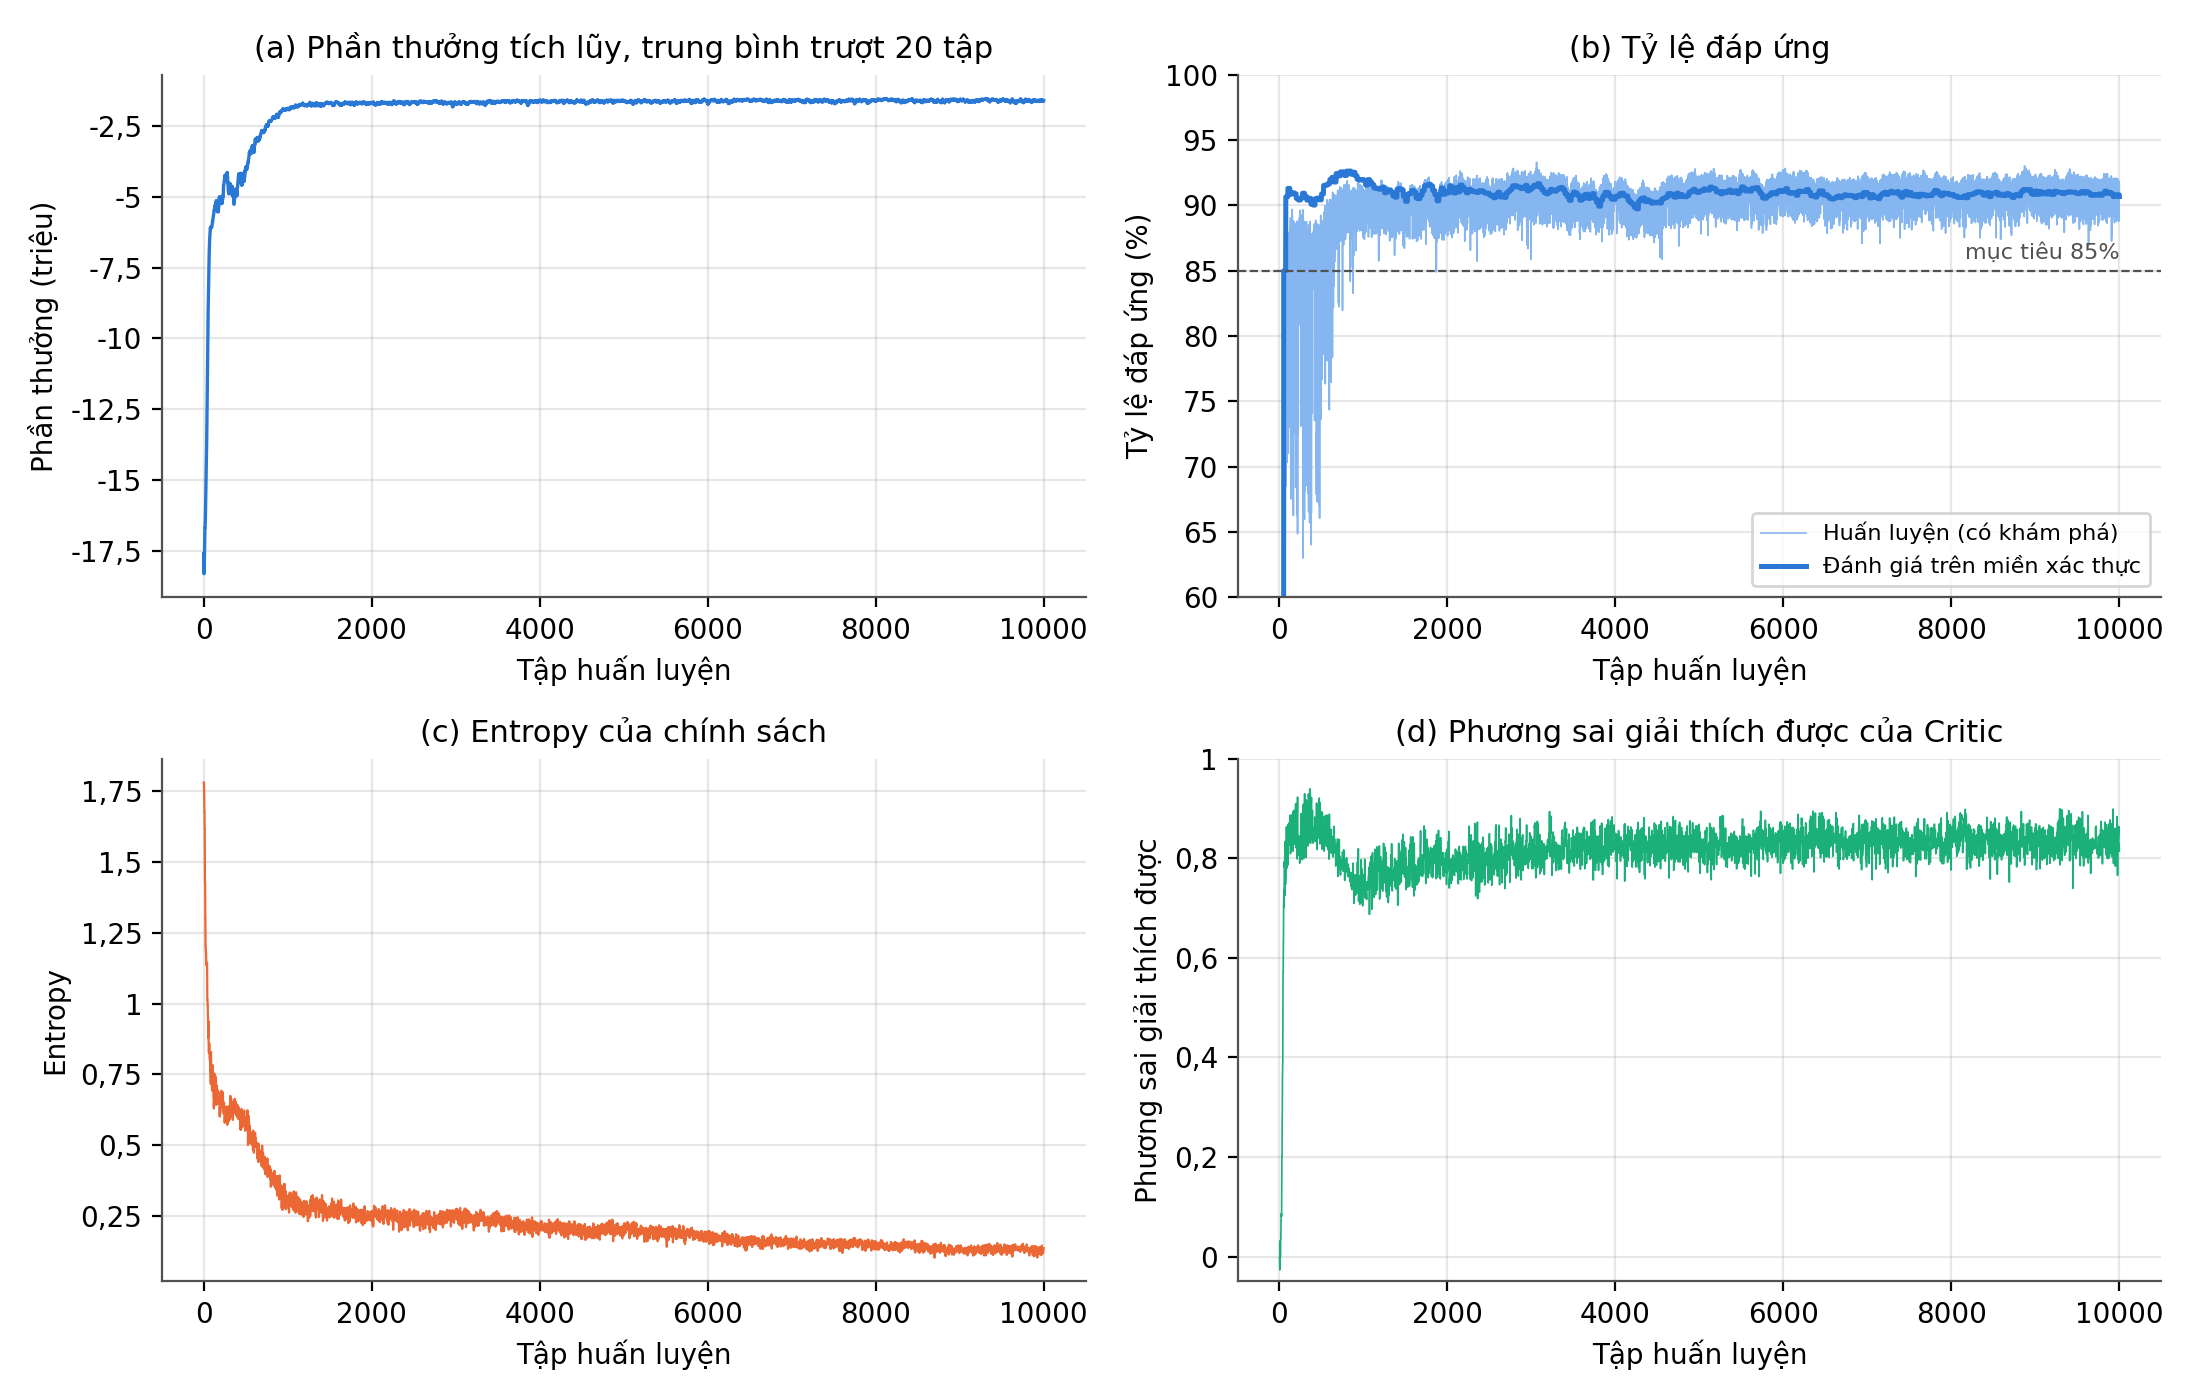
\includegraphics[width=\textwidth]{media/duong_cong_hoc.png}
    \caption{Diễn biến huấn luyện qua 10.000 tập}
    \label{fig:duongCongHoc}
\end{figure}

Hai hạt giống còn lại cho kết quả cùng bậc, với entropy cuối 0,126 và 0,125, phương sai giải thích được 0,84. Ở cả ba hạt giống, chi phí xác thực tốt nhất trong 20\% số tập cuối chỉ lệch 0,2--1,6\% so với phần trước đó. Vì vậy 10.000 tập là đủ để hội tụ.

\subsection{So sánh trực tiếp với các chính sách cổ điển}
\label{subsec:soSanhChiPhi}

Khi mỗi phương pháp dùng cấu hình tốt nhất của mình, IPPO có tổng chi phí xấp xỉ các chính sách cổ điển tốt nhất và có tỷ lệ đáp ứng cao hơn. Trên miền kiểm thử:
\begin{itemize}
    \item IPPO rẻ hơn $(s, S)$ 1,7\% và rẻ hơn EOQ 17,8\%.
    \item IPPO ngang EOQ theo nhóm, Newsvendor và $(s, S)$ theo nhóm, với chênh lệch dưới 1\%.
    \item IPPO đắt hơn Newsvendor theo nhóm 1,6\%.
    \item Tỷ lệ đáp ứng của IPPO là 90,9\%, cao hơn khoảng 4--5 điểm phần trăm so với các chính sách theo nhóm và $(s, S)$. Không chính sách nào xuống dưới 85\%.
\end{itemize}

Kết quả của IPPO là trung bình của ba hạt giống huấn luyện, mỗi hạt giống đánh giá 30 lần. Các chính sách đối chứng là tất định nên kết quả là trung bình trên 30 lần đánh giá dùng chung hạt giống thời gian giao hàng với IPPO.

\begin{table}[htbp]
    \centering
    \caption{Kết quả trên miền kiểm thử}
    \label{tab:ketQuaChiPhi}
    \small
    \setlength{\tabcolsep}{4pt}
    \begin{tabular}{|l|c|c|c|c|c|c|}
        \hline
        Phương pháp & \tbc{Tổng}{chi phí} & \tbc{Tỷ lệ}{đáp ứng} &
        Lưu kho & \tbc{Thiếu}{hàng} & \tbc{Đặt}{hàng} & \tbc{Tràn}{kho} \\
        \hline
        IPPO (3 hạt giống) & \tbc{2.055.442}{$\pm$14.358} & \tbc{90,9\%}{$\pm$0,33\%} &
        1.410.006 & 420.908 & 178.140 & 46.388 \\ \hline
        $(s, S)$ & \tbc{2.091.665}{$\pm$9.258} & \tbc{86,2\%}{$\pm$0,17\%} &
        1.233.832 & 639.569 & 151.834 & 66.430 \\ \hline
        $(s, S)$ theo nhóm & \tbc{2.048.883}{$\pm$8.117} & \tbc{85,9\%}{$\pm$0,16\%} &
        1.171.638 & 655.293 & 176.198 & 45.754 \\ \hline
        EOQ & \tbc{2.500.198}{$\pm$11.329} & \tbc{89,5\%}{$\pm$0,14\%} &
        1.601.700 & 485.725 & 121.240 & 291.533 \\ \hline
        EOQ theo nhóm & \tbc{2.074.745}{$\pm$7.209} & \tbc{85,8\%}{$\pm$0,08\%} &
        1.243.129 & 657.556 & 133.283 & 40.777 \\ \hline
        Newsvendor & \tbc{2.062.190}{$\pm$8.241} & \tbc{87,4\%}{$\pm$0,14\%} &
        1.197.437 & 586.138 & 244.125 & 34.491 \\ \hline
        Newsvendor theo nhóm & \tbc{2.022.942}{$\pm$7.972} & \tbc{85,8\%}{$\pm$0,14\%} &
        1.101.764 & 661.207 & 244.228 & 15.743 \\
        \hline
    \end{tabular}
    \ghichu{Giá trị trung bình. Dấu $\pm$ là độ lệch chuẩn giữa các hạt giống huấn luyện với IPPO, và giữa 30 lần đánh giá với chính sách đối chứng. Chi phí tính bằng đơn vị tiền của mô hình.}
\end{table}

Các chính sách đối chứng tối thiểu chi phí sát ràng buộc 85\%. IPPO cũng tối thiểu chi phí dưới ràng buộc đó nhưng dừng ở mức phục vụ cao hơn. Vì vậy trong phép so sánh này, IPPO nâng được mức phục vụ mà tổng chi phí vẫn ngang các chính sách mạnh nhất.

Kiểm định theo cặp xác nhận các nhận xét trên:
\begin{itemize}
    \item Ba so sánh nhất quán trên cả ba hạt giống là IPPO rẻ hơn $(s, S)$, rẻ hơn EOQ và đắt hơn Newsvendor theo nhóm. Với $(s, S)$ theo nhóm và Newsvendor, dấu của chênh lệch đổi giữa các hạt giống.
    \item Ở hạt giống 1, IPPO rẻ hơn $(s, S)$ 39.169 đơn vị mỗi lần đánh giá (khoảng tin cậy 95\%: 34.404--43.933, $p = 1{,}7 \times 10^{-16}$) và rẻ hơn ở cả 30/30 lần.
    \item Cũng ở hạt giống 1, IPPO đắt hơn Newsvendor theo nhóm 29.554 đơn vị (khoảng tin cậy 95\%: 26.140--32.967) và không lần nào rẻ hơn. Chênh lệch với $(s, S)$ theo nhóm là +0,2\% và không có ý nghĩa ($p = 0{,}088$).
\end{itemize}

Đây là phép so sánh chưa kiểm soát mức phục vụ. Để trả lời Câu hỏi 1, kết quả này cần được đọc cùng phép so sánh ở mục~\ref{subsec:isoService}.

\subsection{Phân tích cơ cấu chi phí}
\label{subsec:coCauChiPhi}

IPPO học được một chiến lược khác với các chính sách cổ điển là tích trữ nhiều hơn để giảm thiếu hàng. Hình~\ref{fig:soSanhBaseline} gồm (a) tổng chi phí, (b) tỷ lệ đáp ứng và (c) chi phí thành phần:
\begin{itemize}
    \item Chi phí lưu kho của IPPO cao hơn $(s, S)$ 14,3\% và cao hơn Newsvendor theo nhóm 28,0\%. Đổi lại, chi phí thiếu hàng thấp hơn hai chính sách này khoảng 34--36\%.
    \item Với $(s, S)$, phần tiết kiệm ở thiếu hàng lớn hơn phần tăng ở lưu kho nên IPPO rẻ hơn. Với các chính sách theo nhóm, hai phần gần như bù nhau.
    \item Chi phí tràn kho của IPPO chiếm khoảng 2,3\% tổng chi phí, thấp hơn $(s, S)$ (3,2\%) và EOQ (11,7\%), nhưng cao hơn hai bản Newsvendor.
    \item IPPO đặt trung bình 35.628 đơn mỗi lần đánh giá, nhiều hơn $(s, S)$ (30.367 đơn) nhưng ít hơn Newsvendor (48.825 đơn).
\end{itemize}

\begin{figure}[H]
    \centering
    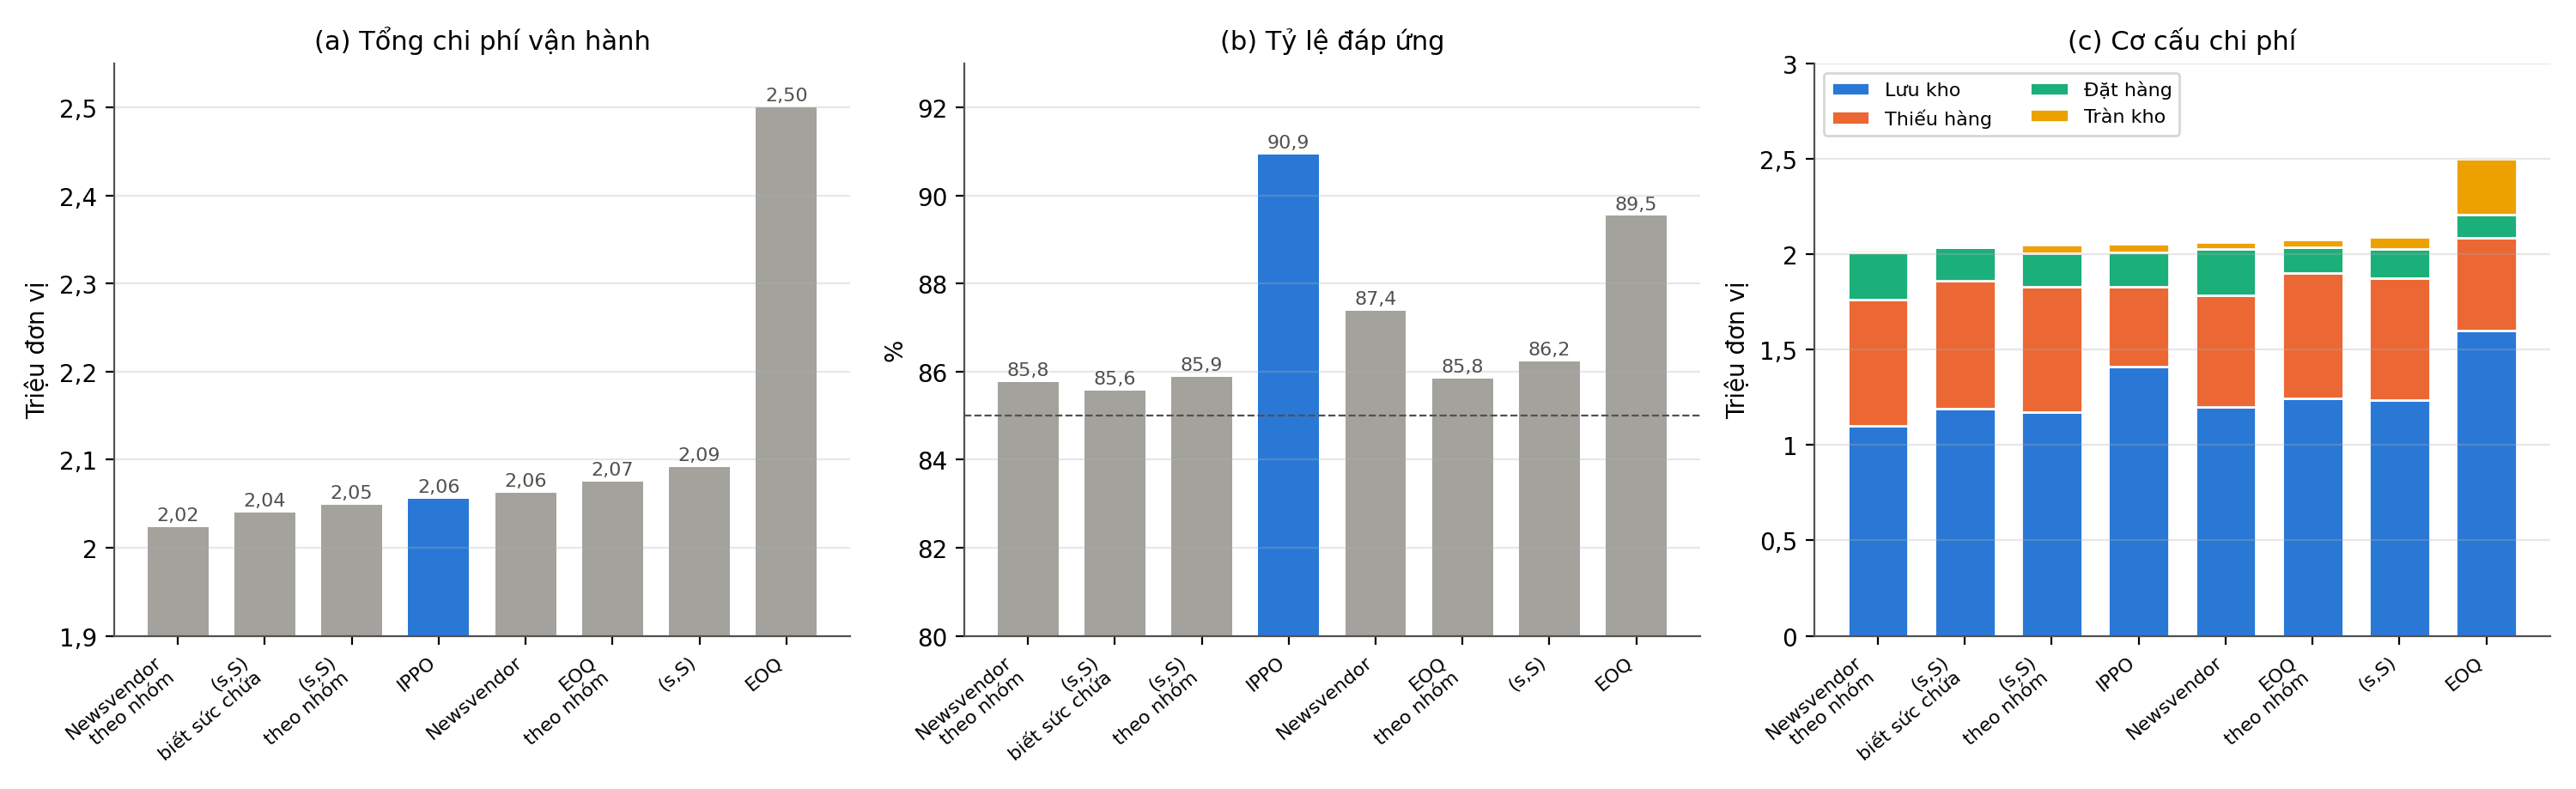
\includegraphics[width=\textwidth]{media/so_sanh_baseline.png}
    \caption{So sánh các phương pháp trên miền kiểm thử}
    \label{fig:soSanhBaseline}
\end{figure}

Mức phục vụ cao hơn của IPPO đến từ lượng tồn kho đệm, không đến từ việc đặt hàng dồn dập. Đây là chiến lược mà hình phạt mức phục vụ (mục~\ref{subsec:fillRate}) khuyến khích. Tác tử giữ tồn kho sát trần sức chứa mà không để tràn kho mất kiểm soát. Tuy vậy, chính sách đã học dựa rất ít vào tín hiệu cấp kho khi suy luận (mục~\ref{subsec:kiemTraStateReward}), nên chưa thể quy kết quả này hoàn toàn cho cơ chế phối hợp qua sức chứa.

\subsection{So sánh ở cùng mức phục vụ}
\label{subsec:isoService}

% [SO-MOI] So cua hat giong 1
Khi phải đạt mức phục vụ ngang IPPO, mọi chính sách cổ điển đều đắt hơn IPPO. Ở phép so sánh trực tiếp, IPPO dừng ở mức phục vụ 90,65\% (hạt giống 1), còn các chính sách đối chứng dừng ở 85,8--89,5\%. Các phương pháp nằm ở những điểm khác nhau trên đường đánh đổi giữa chi phí và mức phục vụ, nên so tổng chi phí là chưa đủ.

Để loại yếu tố này, chi phí của từng chính sách được đọc trên đường biên tại đúng mức phục vụ của IPPO (mục~\ref{subsec:giaoThucIso}):
\begin{itemize}
    \item IPPO rẻ hơn $(s, S)$ 13,3\%, rẻ hơn Newsvendor 8,0\% và rẻ hơn EOQ 22,3\%.
    \item So với các phiên bản theo nhóm, IPPO vẫn rẻ hơn từ 7,3\% đến 9,8\%.
    \item So với $(s, S)$ biết sức chứa, IPPO rẻ hơn 9,2\%.
    \item Newsvendor dự báo là chính sách duy nhất rẻ hơn IPPO, với chênh lệch 4,3\%.
\end{itemize}

\begin{table}[H]
    \centering
    \caption{So sánh ở cùng mức phục vụ}
    \label{tab:isoService}
    \begin{tabular}{|l|c|c|c|}
        \hline
        Phương pháp & Tổng chi phí & \tbc{Tỷ lệ}{đáp ứng} & $\Delta$ IPPO \\
        \hline
        IPPO & 2.052.496 & 90,65\% & --- \\ \hline
        $(s, S)$ & 2.366.664 & 90,65\%$^{\dagger}$ & $-$13,3\% \\ \hline
        $(s, S)$ theo nhóm & 2.213.800 & 90,65\%$^{\dagger}$ & $-$7,3\% \\ \hline
        EOQ & 2.640.010 & 90,60\% & $-$22,3\% \\ \hline
        EOQ theo nhóm & 2.275.502 & 90,75\% & $-$9,8\% \\ \hline
        Newsvendor & 2.230.265 & 90,65\%$^{\dagger}$ & $-$8,0\% \\ \hline
        Newsvendor theo nhóm & 2.243.057 & 90,65\%$^{\dagger}$ & $-$8,5\% \\ \hline
        Newsvendor dự báo & 1.968.561 & 90,65\%$^{\dagger}$ & +4,3\% \\ \hline
        $(s, S)$ biết sức chứa & 2.260.819 & 90,65\%$^{\dagger}$ & $-$9,2\% \\
        \hline
    \end{tabular}
    \ghichu{Cột $\Delta$ IPPO là chênh lệch chi phí của IPPO so với chính sách đó, âm là IPPO rẻ hơn. Dấu $^{\dagger}$: chi phí được nội suy trên đường biên.}
\end{table}

Hai phép so sánh được đặt trên cùng mặt phẳng chi phí và mức phục vụ ở Hình~\ref{fig:danhDoi}. Dấu chữ thập xám là cấu hình tối thiểu chi phí của các chính sách đối chứng, dấu tròn xanh dương là các chính sách đã chỉnh về cùng mức phục vụ, chấm xanh lá là IPPO.

\begin{figure}[H]
    \centering
    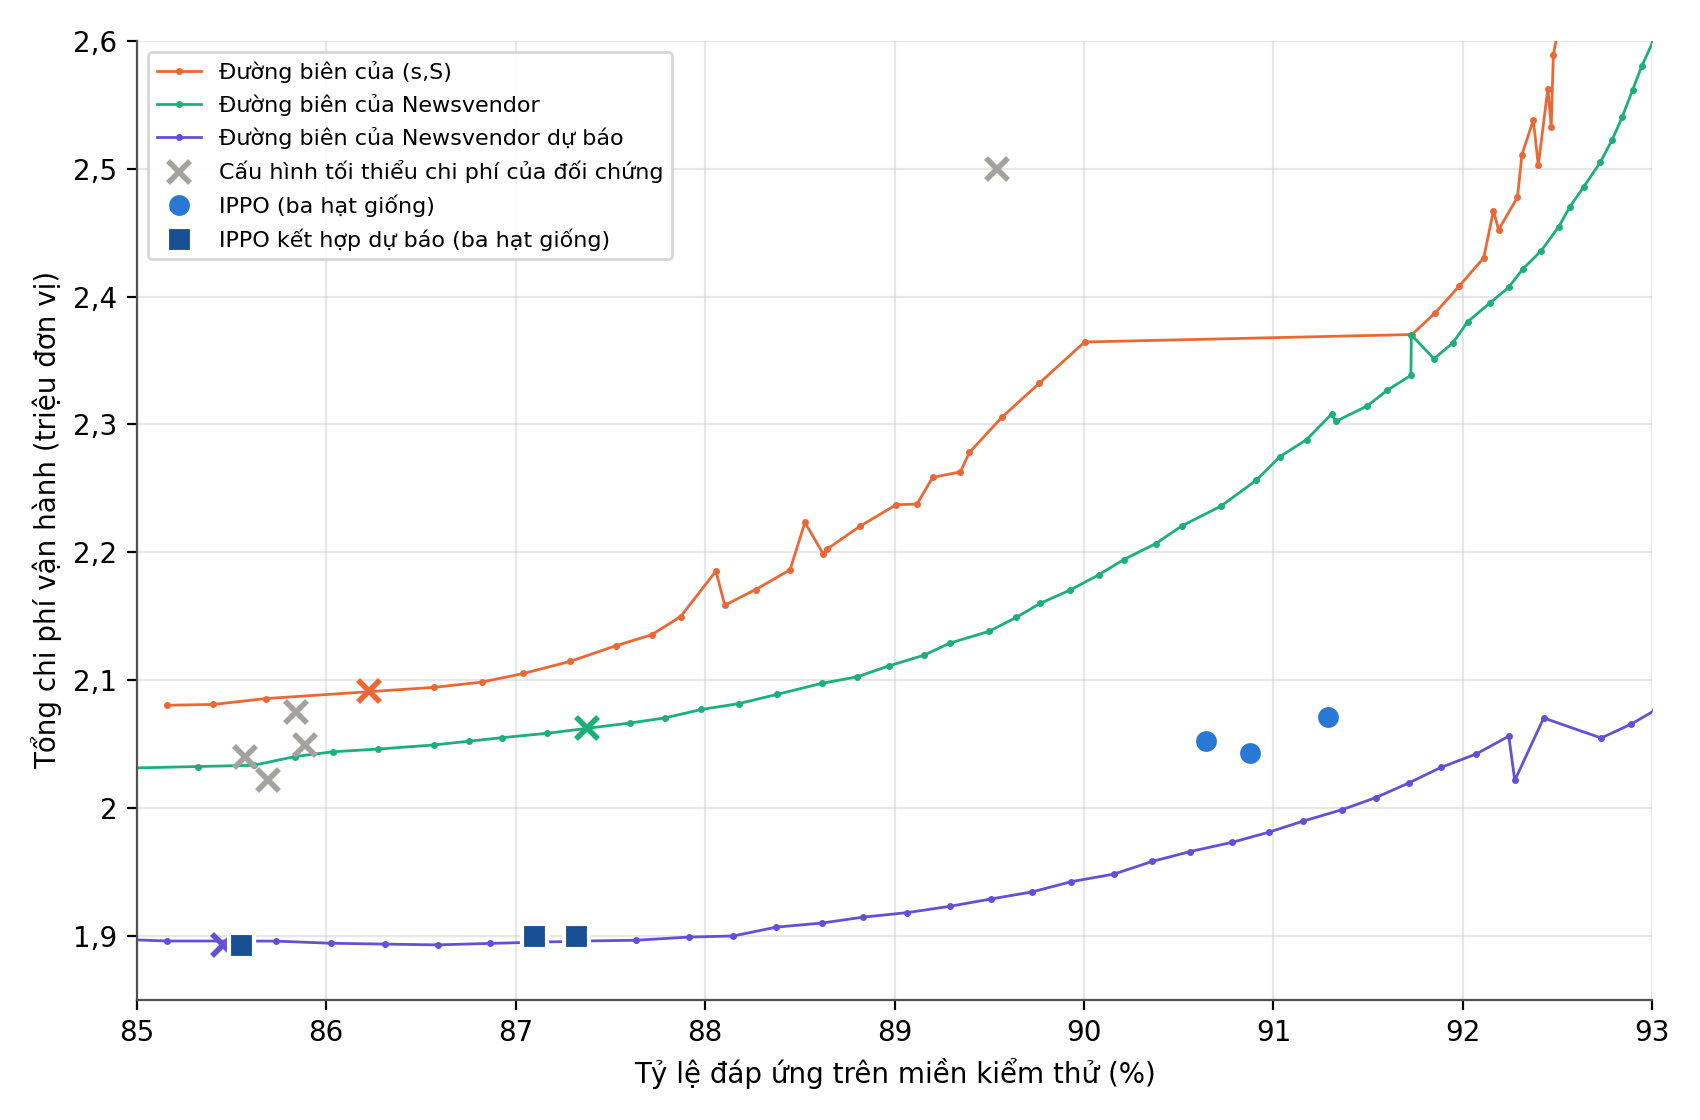
\includegraphics[width=0.72\textwidth]{media/danh_doi_chi_phi_dich_vu.png}
    \caption{Đánh đổi giữa chi phí và mức phục vụ}
    \label{fig:danhDoi}
\end{figure}

Khoảng cách bắt nguồn từ cách điều chỉnh của chính sách cổ điển. Muốn nâng mức phục vụ, chúng chỉ có thể tăng tham số an toàn $\alpha$ hoặc $CR$ đồng loạt cho cả hệ thống hoặc cả nhóm, nên tồn kho tăng ở mọi mặt hàng trong nhóm. IPPO điều chỉnh theo trạng thái từng cặp, nên chỉ tích trữ thêm ở những cặp cần.

\subsection{So sánh với chính sách có thêm thông tin}
\label{subsec:soSanhThongTin}

% [SO-MOI] So cua hat giong 1, thay bang ket qua nhieu hat giong va duong bien day du
Khi chính sách đối chứng có thêm dự báo nhu cầu, IPPO không còn rẻ hơn. Các kết quả dưới đây dùng mô hình của hạt giống 1.

\begin{table}[H]
    \centering
    \caption{So sánh với chính sách có thêm thông tin}
    \label{tab:soSanhThongTin}
    \small
    \begin{tabular}{|l|c|c|c|}
        \hline
        Chính sách & Tổng chi phí & \tbc{Tỷ lệ}{đáp ứng} & $\Delta$ IPPO \\
        \hline
        IPPO & 2.052.496 & 90,65\% & --- \\ \hline
        $(s, S)$ biết sức chứa & 2.153.173 & 86,1\% & $-$4,7\% \\ \hline
        Newsvendor dự báo & 1.899.732 & 88,1\% & +8,0\% \\ \hline
        Newsvendor dự báo, cùng mức phục vụ & 1.968.561 & 90,65\% & +4,3\% \\ \hline
        Biết trước nhu cầu & 1.358.864 & 93,6\% & +51,0\% \\
        \hline
    \end{tabular}
    \ghichu{Cột $\Delta$ IPPO là chênh lệch chi phí của IPPO so với chính sách đó, âm là IPPO rẻ hơn.}
\end{table}

Có ba nhận xét từ kết quả này:
\begin{itemize}
    \item Giảm đều lượng đặt theo chỗ trống của kho giúp $(s, S)$ rẻ hơn khi so ở cùng mức phục vụ, nhưng vẫn đắt hơn IPPO 9,2\%. Biết sức chứa theo cách đơn giản này chưa đủ để bắt kịp IPPO.
    \item Chính sách dùng dự báo rẻ hơn IPPO, kể cả khi hai bên có mức phục vụ gần nhau. IPPO chỉ nhận lịch sử 7 ngày và lịch của ngày hiện tại, còn mô hình dự báo được học từ nhiều đặc trưng hơn trên cả 300 cặp.
    \item Biết trước nhu cầu giảm được khoảng một phần ba chi phí so với IPPO mà tỷ lệ đáp ứng còn cao hơn. Thông tin về nhu cầu tương lai là phần có giá trị lớn nhất, đây là lý do nhóm thử các biến thể có dự báo.
\end{itemize}

\subsection{Kết hợp IPPO và chính sách dự báo}
\label{subsec:ketHop}

% [SO-MOI] So cua hat giong 1, thay bang ket qua nhieu hat giong
Dùng chính sách dự báo cho nhóm bán chậm và giữ IPPO cho nhóm bán nhanh rẻ hơn dùng riêng IPPO. Để biết học tăng cường thêm được gì, chi phí và mức phục vụ được tách theo bốn nhóm quy mô nhu cầu.

\begin{table}[H]
    \centering
    \caption{IPPO và Newsvendor dự báo theo nhóm nhu cầu}
    \label{tab:ketHop}
    \small
    \begin{tabular}{|l|c|c|c|c|}
        \hline
        \multirow{2}{*}{Nhóm nhu cầu} & \multicolumn{2}{c|}{IPPO} & \multicolumn{2}{c|}{Newsvendor dự báo} \\
        \cline{2-5}
        & Chi phí & Tỷ lệ đáp ứng & Chi phí & Tỷ lệ đáp ứng \\
        \hline
        Rất thấp ($<0{,}5$) & 248.587 & 74,2\% & 254.448 & 78,2\% \\ \hline
        Thấp (0,5--2) & 470.140 & 83,2\% & 443.355 & 85,3\% \\ \hline
        Trung bình (2--10) & 485.451 & 89,5\% & 445.004 & 86,7\% \\ \hline
        Cao ($\ge 10$) & 848.318 & 95,8\% & 756.926 & 91,1\% \\ \hline
        Toàn hệ thống & 2.052.496 & 90,65\% & 1.899.732 & 88,1\% \\
        \hline
    \end{tabular}
\end{table}

Chính sách dự báo chiếm ưu thế ở hai nhóm bán chậm. Ở hai nhóm bán nhanh, IPPO có mức phục vụ cao hơn nhưng tốn thêm chi phí. Từ đó nhóm xây dựng chính sách kết hợp theo các bước sau:
\begin{itemize}
    \item Mỗi nhóm nhu cầu dùng IPPO hoặc một cấu hình Newsvendor dự báo trên đường biên. Các cách gán được quét trên miền xác thực để tạo đường biên chi phí--mức phục vụ của chính sách kết hợp.
    \item Các chính sách chạy chung trong một lần mô phỏng, vì các cặp vẫn chia sẻ sức chứa của cùng một kho.
    \item Để so sánh công bằng, Newsvendor dự báo cũng được chọn cấu hình theo nhóm theo đúng cách này nhưng không có IPPO.
    \item Không cần huấn luyện lại. Chính sách kết hợp chỉ dùng mô hình đã học và mô hình dự báo đã có.
\end{itemize}

Đọc trên đường biên tại mức phục vụ 90,65\% của IPPO, kết quả trên miền kiểm thử như sau:
\begin{itemize}
    \item Trong các cách gán gần mức này, IPPO chỉ được chọn cho nhóm nhu cầu cao, ba nhóm còn lại dùng chính sách dự báo.
    \item Chính sách kết hợp có chi phí 1.987.598, rẻ hơn IPPO 3,2\%.
    \item Chính sách kết hợp vẫn đắt hơn Newsvendor dự báo 1,0\%. Khoảng cách đã giảm từ mức 4,3\% của IPPO nhưng chưa đảo chiều.
    \item Newsvendor dự báo theo nhóm có chi phí 1.965.309, gần như không đổi so với 1.968.561 của bản một cấu hình.
\end{itemize}

Kết quả này cho thấy ở nhóm bán chậm, quy tắc đặt hàng theo dự báo là đủ. Nhóm nhu cầu cao là nhóm duy nhất mà IPPO tiến gần chính sách dự báo, nhưng trên mô hình này IPPO chưa tạo được lợi thế chi phí so với một cấu hình dự báo có hệ số an toàn cao hơn.

\subsection{Hiệu năng theo giai đoạn nhu cầu}
\label{subsec:hanChe}

Học tăng cường không rẻ hơn ở mọi giai đoạn nhu cầu, nhưng giữ mức phục vụ bền hơn khi nhu cầu biến động. Các kết quả ở trên lấy trung bình trên cả miền kiểm thử. Thực nghiệm này tách kết quả theo loại ngày để xem chính sách cổ điển có tốt hơn khi nhu cầu ổn định hay không. Các chính sách đã có được đánh giá lại, không huấn luyện lại.

\subsubsection{Thiết kế thực nghiệm}

Mỗi ngày trong miền kiểm thử được gán nhãn theo hai cách:
\begin{itemize}
    \item Theo mức biến động. Với mỗi ngày $t$ và mỗi kho $w$, độ lệch $\bigl|D_t^{(w)} / \overline{D}_{28}^{(w)} - 1\bigr|$ giữa tổng nhu cầu của kho và trung bình 28 ngày trước đó được tính rồi lấy trung bình trên 10 kho. Các ngày được chia theo tam phân vị thành ba nhóm ổn định ($\le 20{,}3\%$), trung bình và biến động ($> 30{,}8\%$), mỗi nhóm khoảng 164 ngày.
    \item Theo lịch. Các nhóm gồm ngày có sự kiện (43 ngày), ngày SNAP (240 ngày), cuối tuần (141 ngày), mùa lễ tháng 11--12 (61 ngày) và ngày thường không sự kiện, không SNAP, không cuối tuần (164 ngày).
\end{itemize}

Ngoài các giai đoạn tự nhiên, thực nghiệm tạo sốc cầu nhân tạo: nhu cầu của 28 ngày (1650--1677) được nhân với 1,5 (tăng đột biến) hoặc 0,5 (sụt giảm). Tỷ lệ đáp ứng và chi phí được đo trong 28 ngày trước, trong và sau cú sốc. Bên cạnh sáu chính sách đối chứng tinh chỉnh trực tiếp, thực nghiệm dùng thêm hai chính sách đã chỉnh về cùng mức phục vụ với IPPO (mục~\ref{subsec:isoService}).
% [SO-MOI] Them dong Newsvendor du bao va bien the he so an toan tren nen du bao vao bang soc cau

\begin{table}[H]
    \centering
    \caption{Tỷ lệ đáp ứng và chi phí mỗi ngày theo giai đoạn nhu cầu}
    \label{tab:theoGiaiDoan}
    \small
    \setlength{\tabcolsep}{4pt}
    \begin{tabular}{|l|c|c|c|c|c|c|c|}
        \hline
        \multirow{2}{*}{Giai đoạn} &
        \multicolumn{2}{c|}{IPPO} &
        \multicolumn{2}{c|}{$(s,S)$ trực tiếp} &
        \multicolumn{2}{c|}{$(s,S)$ cùng mức} &
        \multirow{2}{*}{Chênh} \\
        \cline{2-7}
        & TLĐƯ & CP/ngày & TLĐƯ & CP/ngày & TLĐƯ & CP/ngày & \\
        \hline
        Ổn định        & 91,6\% & 3.874 & 89,2\% & 3.896 & 94,3\% & 5.475 & $-$29,2\% \\ \hline
        Trung bình     & 90,9\% & 3.981 & 86,8\% & 4.117 & 93,2\% & 5.502 & $-$27,6\% \\ \hline
        Biến động      & 89,4\% & 4.684 & 82,7\% & 4.767 & 90,5\% & 5.899 & $-$20,6\% \\ \hline
        Ngày có sự kiện & 88,9\% & 4.439 & 80,6\% & 4.801 & 89,5\% & 5.738 & $-$22,6\% \\ \hline
        Ngày SNAP      & 90,4\% & 4.278 & 86,1\% & 4.329 & 92,6\% & 5.706 & $-$25,0\% \\ \hline
        Cuối tuần      & 90,5\% & 4.408 & 81,8\% & 4.824 & 90,9\% & 5.567 & $-$20,8\% \\ \hline
        Mùa lễ (T11--12) & 88,3\% & 5.057 & 84,7\% & 4.676 & 90,4\% & 6.332 & $-$20,1\% \\ \hline
        Ngày thường    & 91,1\% & 3.962 & 89,0\% & 3.943 & 94,0\% & 5.540 & $-$28,5\% \\ \hline
        Toàn miền kiểm thử & 90,6\% & 4.180 & 86,2\% & 4.260 & 92,7\% & 5.626 & $-$25,7\% \\
        \hline
    \end{tabular}
    \ghichu{TLĐƯ: tỷ lệ đáp ứng. CP/ngày: chi phí vận hành trung bình mỗi ngày. ``Cùng mức'': chỉnh về cùng mức phục vụ với IPPO. Cột cuối là chênh lệch chi phí của IPPO so với $(s,S)$ cùng mức phục vụ, âm là IPPO rẻ hơn. 30 lần đánh giá trên miền kiểm thử.}
\end{table}

\begin{figure}[H]
    \centering
    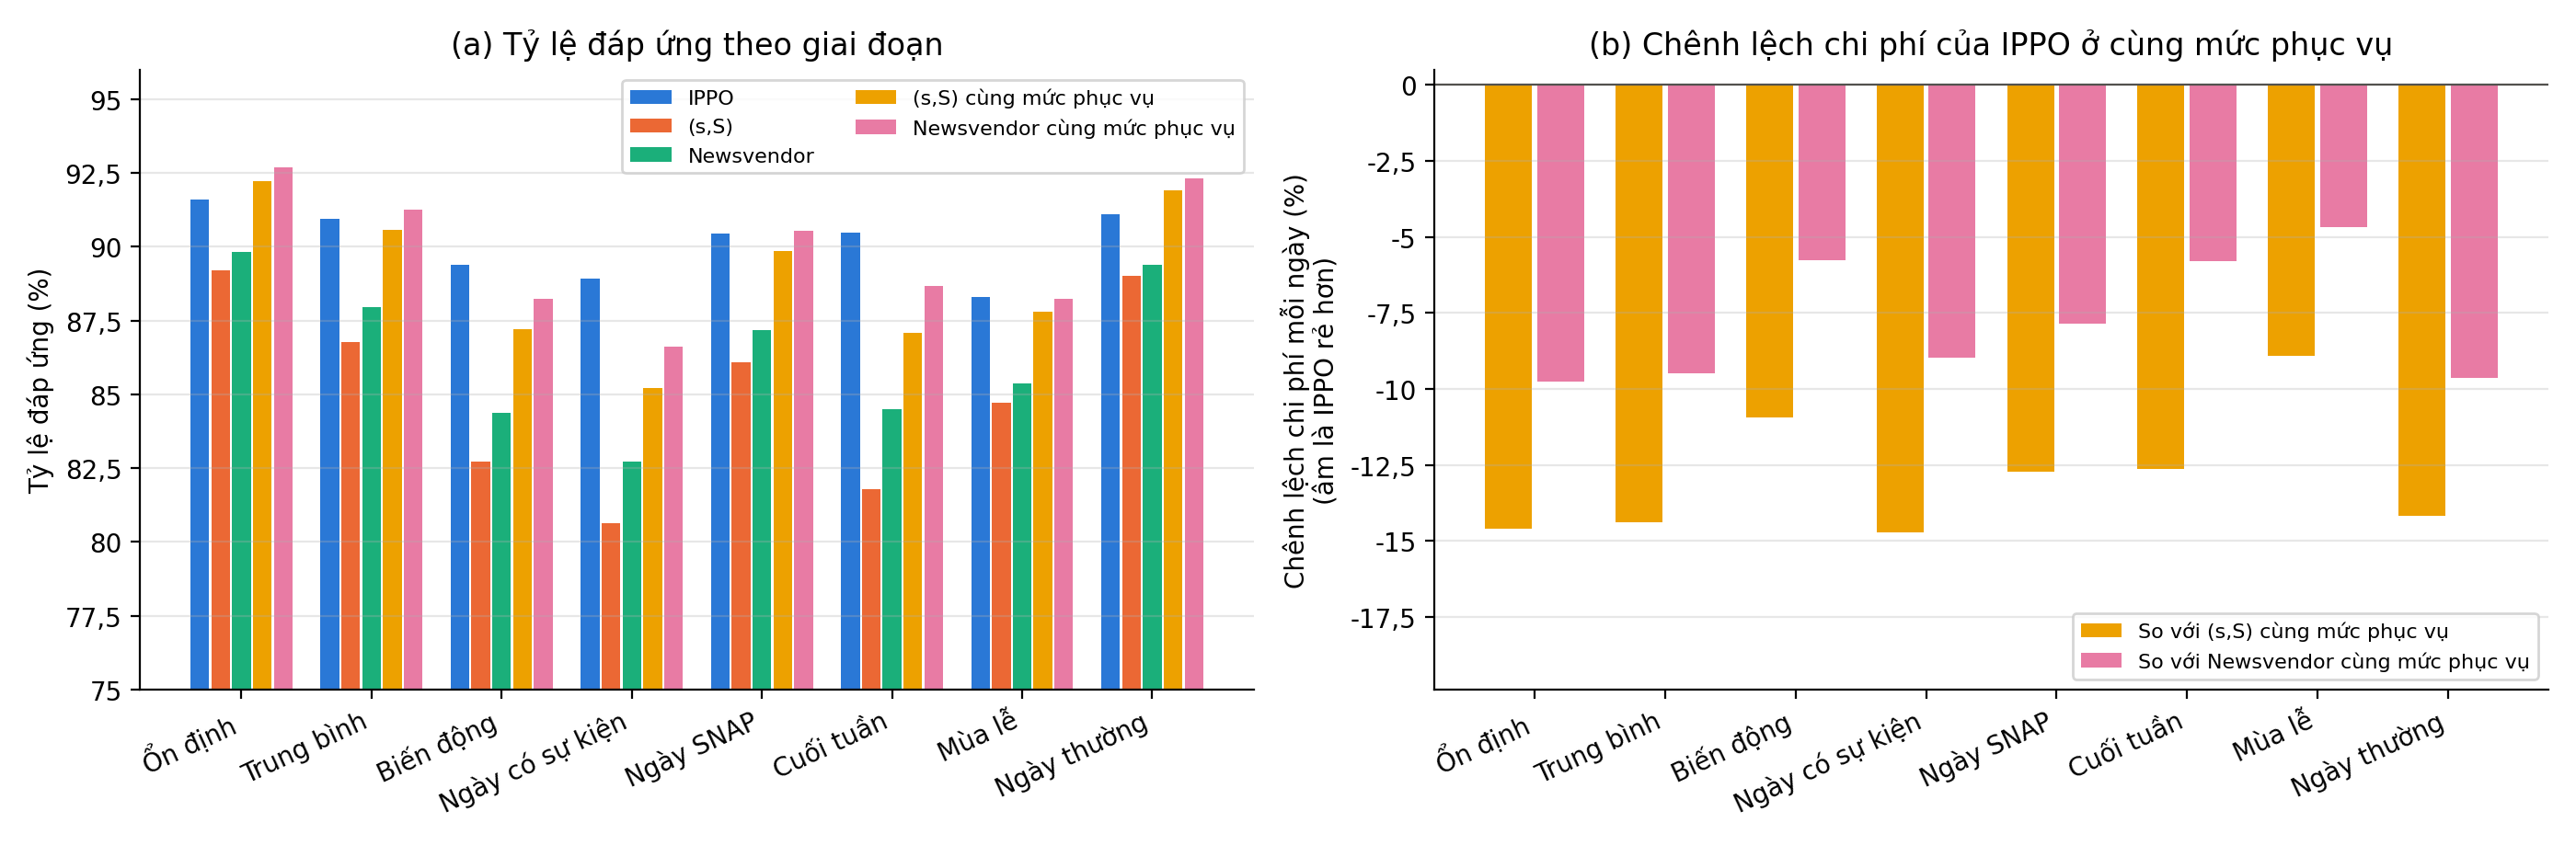
\includegraphics[width=\textwidth]{media/hinh_theo_giai_doan_nhu_cau.png}
    \caption{Tỷ lệ đáp ứng và chênh lệch chi phí theo giai đoạn nhu cầu}
    \label{fig:theoGiaiDoan}
\end{figure}

\subsubsection{Kết quả theo giai đoạn tự nhiên}

Hình~\ref{fig:theoGiaiDoan} gồm (a) tỷ lệ đáp ứng theo giai đoạn và (b) chênh lệch chi phí mỗi ngày của IPPO so với hai chính sách cùng mức phục vụ. Các ngày gần nhau không độc lập vì nhu cầu có tự tương quan, nên khoảng tin cậy 95\% của từng chênh lệch được ước lượng bằng bootstrap theo khối 7 ngày, lấy mẫu lại nguyên từng tuần 2.000 lần. IPPO được so với $(s,S)$ tinh chỉnh trực tiếp, $(s,S)$ cùng mức phục vụ và Newsvendor theo nhóm, chính sách mạnh nhất ở phép so sánh trực tiếp.

\begin{table}[htbp]
    \centering
    \caption{Chênh lệch chi phí mỗi ngày của IPPO và khoảng tin cậy 95\%}
    \label{tab:ciGiaiDoan}
    \small
    \begin{tabular}{|l|c|c|c|}
        \hline
        Giai đoạn & So với $(s,S)$ & \tbc{So với $(s,S)$}{cùng mức phục vụ} & \tbc{So với Newsvendor}{theo nhóm} \\
        \hline
        Ổn định          & \tbc{$-$0,6\%}{$[-2{,}3;\ +1{,}3]$} & \tbc{$-$29,2\%}{$[-31{,}0;\ -27{,}4]^{*}$} & \tbc{+2,3\%}{$[+0{,}7;\ +4{,}0]^{*}$} \\ \hline
        Trung bình       & \tbc{$-$3,3\%}{$[-5{,}8;\ -0{,}6]^{*}$} & \tbc{$-$27,6\%}{$[-30{,}0;\ -24{,}8]^{*}$} & \tbc{+0,3\%}{$[-1{,}8;\ +2{,}6]$} \\ \hline
        Biến động        & \tbc{$-$1,7\%}{$[-7{,}5;\ +3{,}7]$} & \tbc{$-$20,6\%}{$[-23{,}6;\ -17{,}7]^{*}$} & \tbc{+1,8\%}{$[-2{,}5;\ +5{,}9]$} \\ \hline
        Ngày có sự kiện  & \tbc{$-$7,5\%}{$[-14{,}7;\ -0{,}2]^{*}$} & \tbc{$-$22,6\%}{$[-26{,}0;\ -19{,}2]^{*}$} & \tbc{$-$3,4\%}{$[-9{,}4;\ +2{,}5]$} \\ \hline
        Ngày SNAP        & \tbc{$-$1,2\%}{$[-4{,}6;\ +2{,}5]$} & \tbc{$-$25,0\%}{$[-27{,}5;\ -22{,}3]^{*}$} & \tbc{+1,5\%}{$[-1{,}0;\ +4{,}1]$} \\ \hline
        Cuối tuần        & \tbc{$-$8,6\%}{$[-12{,}9;\ -4{,}0]^{*}$} & \tbc{$-$20,8\%}{$[-23{,}1;\ -18{,}6]^{*}$} & \tbc{$-$2,6\%}{$[-6{,}2;\ +1{,}1]$} \\ \hline
        Mùa lễ (T11--12) & \tbc{+8,2\%}{$[-3{,}3;\ +17{,}8]$} & \tbc{$-$20,1\%}{$[-28{,}1;\ -12{,}7]^{*}$} & \tbc{+10,1\%}{$[+2{,}5;\ +16{,}2]^{*}$} \\ \hline
        Ngày thường      & \tbc{+0,5\%}{$[-2{,}9;\ +3{,}8]$} & \tbc{$-$28,5\%}{$[-31{,}3;\ -25{,}2]^{*}$} & \tbc{+3,3\%}{$[+1{,}0;\ +5{,}7]^{*}$} \\
        \hline
    \end{tabular}
    \ghichu{Bootstrap theo khối 7 ngày, 2.000 lần lấy mẫu lại. Âm là IPPO rẻ hơn. Dấu $^{*}$: khoảng tin cậy không chứa 0.}
\end{table}

Kết quả theo giai đoạn cho thấy:
\begin{itemize}
    \item Khi nhu cầu ổn định, chính sách cổ điển cạnh tranh được. Ở ngày ổn định và ngày thường, IPPO ngang $(s,S)$ trực tiếp nhưng đắt hơn Newsvendor theo nhóm 2,3\% và 3,3\%, có ý nghĩa thống kê. Khi nhu cầu gần trung bình trượt, công thức $s = \mu_L + z\sigma_L$ là xấp xỉ tốt.
    \item Khi nhu cầu biến động, ưu thế của IPPO nằm ở độ bền của mức phục vụ. Từ nhóm ổn định sang nhóm biến động, tỷ lệ đáp ứng của IPPO giảm 2,2 điểm, của $(s,S)$ trực tiếp giảm 6,5 điểm và của $(s,S)$ cùng mức phục vụ giảm 3,8 điểm.
    \item Ở ngày có sự kiện và cuối tuần, IPPO rẻ hơn $(s,S)$ trực tiếp 7,5\% và 8,6\%, kèm tỷ lệ đáp ứng cao hơn khoảng 8--9 điểm. Chênh lệch so với Newsvendor theo nhóm ở các ngày này không có ý nghĩa.
    \item Ở cùng mức phục vụ, IPPO rẻ hơn trong mọi giai đoạn, 20,1--29,2\% so với $(s,S)$ và 12,7--20,1\% so với Newsvendor. Hai chính sách này giữ tỷ lệ đáp ứng cao hơn IPPO ở hầu hết các nhóm ngày, nên khoảng cách bị phóng đại như đã nêu ở mục~\ref{subsec:isoService}.
\end{itemize}

Mùa lễ cuối năm là giai đoạn yếu nhất của IPPO. Tỷ lệ đáp ứng thấp nhất (88,3\%), và IPPO đắt hơn Newsvendor theo nhóm 10,1\%, có ý nghĩa thống kê. Mùa lễ chỉ gồm 9 tuần trong miền kiểm thử và miền huấn luyện chỉ chứa khoảng ba mùa lễ, nên đây là điểm yếu cần theo dõi. Tác tử cũng gần như không khai thác đặc trưng lịch (mục~\ref{subsec:kiemTraStateReward}).

\begin{table}[H]
    \centering
    \caption{Tỷ lệ đáp ứng và chi phí mỗi ngày quanh cú sốc cầu}
    \label{tab:socCau}
    \small
    \begin{tabular}{|l|c|c|c|c|c|c|}
        \hline
        \multirow{2}{*}{Chính sách} &
        \multicolumn{3}{c|}{Sốc tăng $\times 1{,}5$} &
        \multicolumn{3}{c|}{Sốc giảm $\times 0{,}5$} \\
        \cline{2-7}
        & Trước & Trong & Sau & Trước & Trong & Sau \\
        \hline
        IPPO & \tbc{91,6\%}{(3.724)} & \tbc{83,5\%}{($\mathbf{5.451}$)} & \tbc{$\mathbf{93{,}3\%}$}{(4.150)} & \tbc{91,6\%}{(3.724)} & \tbc{97,8\%}{(3.354)} & \tbc{$\mathbf{90{,}8\%}$}{(3.865)} \\ \hline
        $(s,S)$ trực tiếp & \tbc{88,6\%}{(3.925)} & \tbc{81,2\%}{(6.552)} & \tbc{89,6\%}{(4.253)} & \tbc{88,6\%}{(3.925)} & \tbc{91,7\%}{(2.680)} & \tbc{82,9\%}{(4.291)} \\ \hline
        Newsvendor trực tiếp & \tbc{90,2\%}{(3.809)} & \tbc{83,7\%}{(6.278)} & \tbc{91,5\%}{(4.121)} & \tbc{90,2\%}{(3.809)} & \tbc{92,0\%}{(2.579)} & \tbc{83,4\%}{(4.285)} \\ \hline
        $(s,S)$ cùng mức phục vụ & \tbc{94,3\%}{(5.346)} & \tbc{84,8\%}{(9.392)} & \tbc{92,2\%}{(6.578)} & \tbc{94,3\%}{(5.346)} & \tbc{97,8\%}{(3.590)} & \tbc{90,5\%}{(5.290)} \\ \hline
        \tbl{Newsvendor cùng}{mức phục vụ} & \tbc{94,6\%}{(4.617)} & \tbc{86,1\%}{(8.169)} & \tbc{93,3\%}{(5.637)} & \tbc{94,6\%}{(4.617)} & \tbc{96,6\%}{(3.189)} & \tbc{89,2\%}{(4.820)} \\
        \hline
    \end{tabular}
    \ghichu{Mỗi ô ghi tỷ lệ đáp ứng và, trong ngoặc, chi phí mỗi ngày trong 28 ngày trước, trong và sau cú sốc. Chữ đậm đánh dấu giá trị tốt nhất của IPPO được nhắc trong bài.}
\end{table}

\begin{figure}[H]
    \centering
    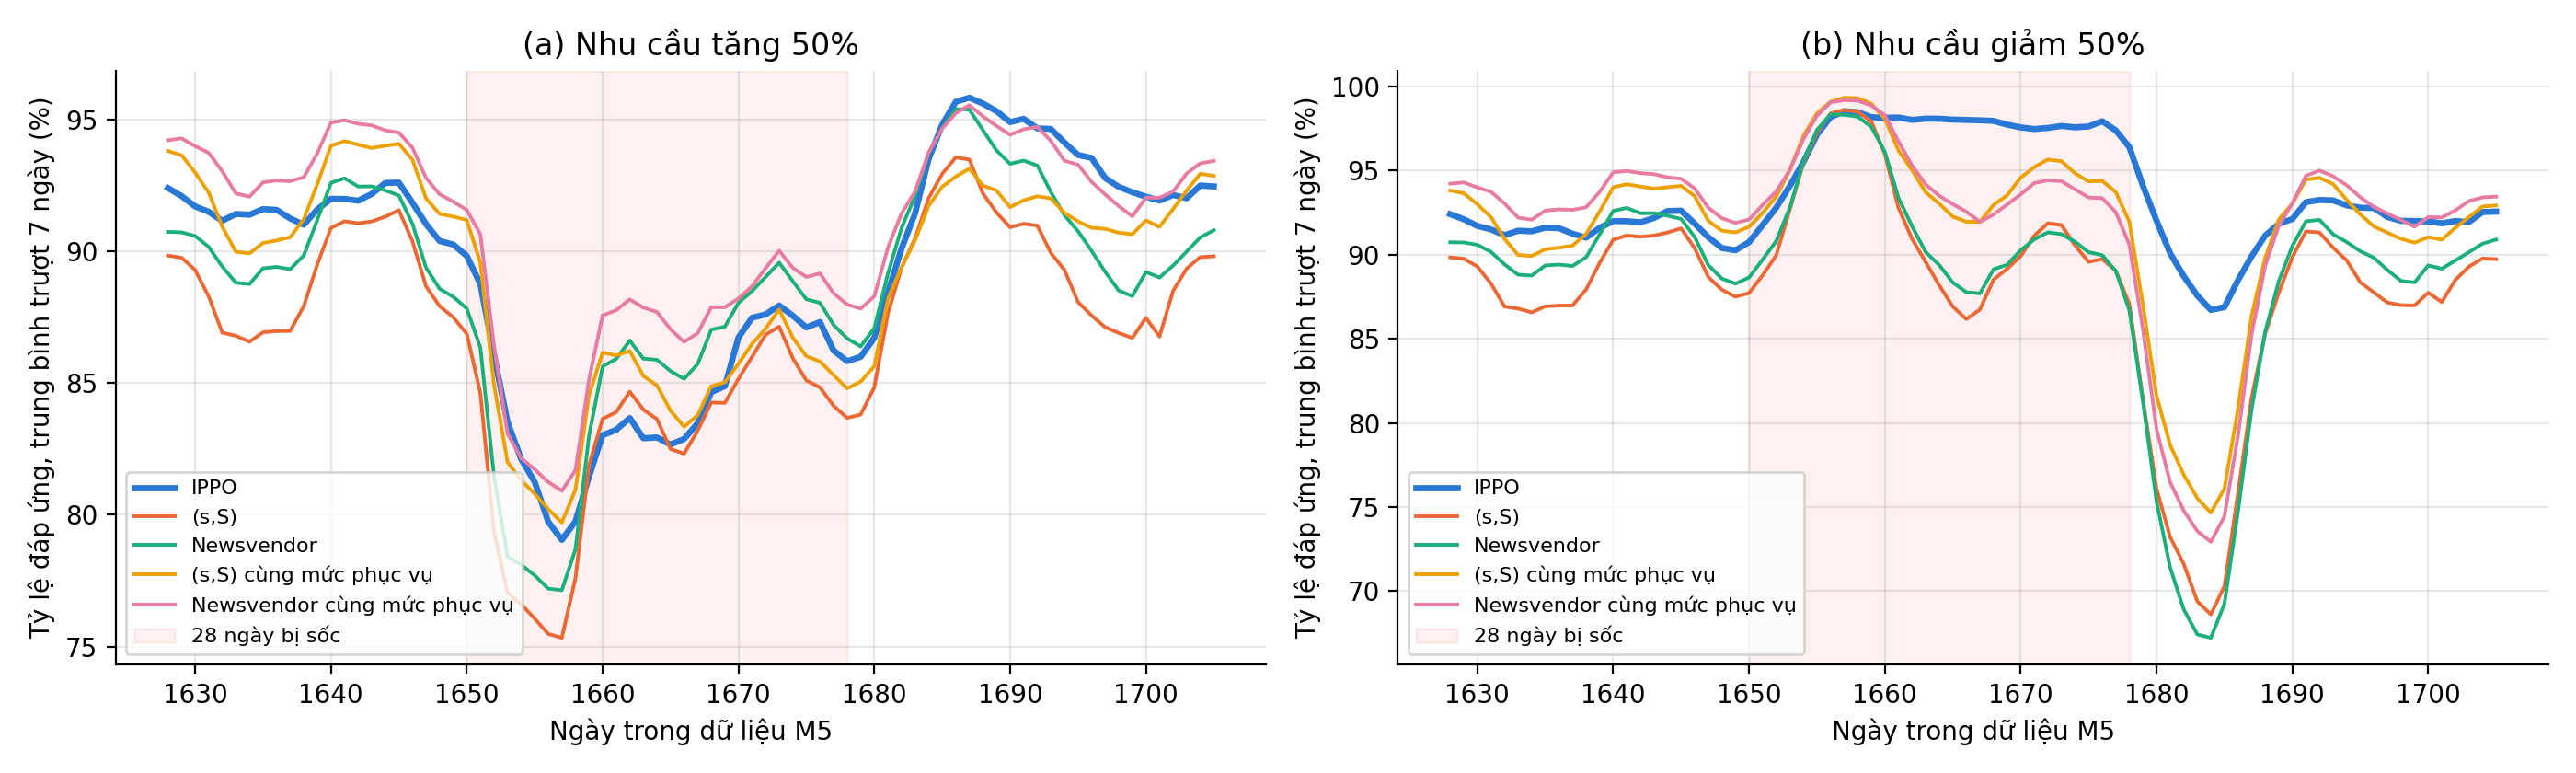
\includegraphics[width=\textwidth]{media/hinh_soc_cau.png}
    \caption{Tỷ lệ đáp ứng theo ngày quanh cú sốc cầu}
    \label{fig:socCau}
\end{figure}

\subsubsection{Kết quả khi có sốc cầu}

IPPO phục hồi tốt hơn sau cú sốc, nhất là khi nhu cầu sụt rồi quay lại. Hình~\ref{fig:socCau} vẽ tỷ lệ đáp ứng làm mượt bằng trung bình trượt 7 ngày, với vùng tô đỏ là 28 ngày bị sốc:
\begin{itemize}
    \item Khi nhu cầu tăng 50\%, mọi chính sách mất khoảng 6--10 điểm tỷ lệ đáp ứng. Ở mức phục vụ gần như nhau, IPPO tốn ít hơn Newsvendor trực tiếp 13,2\% và $(s,S)$ trực tiếp 16,8\%. Sau cú sốc, IPPO phục hồi lên 93,3\%.
    \item Khi nhu cầu sụt 50\% rồi hồi phục, $(s,S)$ và Newsvendor trực tiếp giảm xuống 82,9\% và 83,4\%. Hai chính sách cùng mức phục vụ giảm xuống 90,5\% và 89,2\%. IPPO giữ 90,8\%.
\end{itemize}

Khi nhu cầu hồi phục, ước lượng $\mu$ và $\sigma$ từ cửa sổ 7 ngày của chính sách cổ điển vẫn phản ánh giai đoạn nhu cầu thấp nên chúng đặt quá ít. IPPO kết hợp lịch sử 7 ngày với đặc trưng quy mô dài hạn $\log(1 + \bar{D}^{(i)})$, nên bền hơn trước nhiễu ngắn hạn. Đổi lại, IPPO có thể phản ứng chậm hơn nếu nhu cầu thay đổi lâu dài.

\subsubsection{Nhận xét chung}

Học tăng cường không đạt chi phí thấp hơn ở mọi giai đoạn. Khi nhu cầu ổn định, chính sách cổ điển tinh chỉnh tốt rẻ hơn IPPO vài phần trăm, và mùa lễ là giai đoạn IPPO kém nhất. Ưu thế của IPPO tập trung ở ba điểm:
\begin{itemize}
    \item Mức phục vụ bền khi nhu cầu biến động và khi hồi phục sau cú sụt.
    \item Chi phí thấp hơn $(s,S)$ ở ngày có sự kiện và cuối tuần.
    \item Chi phí thấp hơn các chính sách cùng mức phục vụ khi chống đỡ sốc tăng cầu.
\end{itemize}

Miền kiểm thử chỉ dài 491 ngày và mùa lễ chỉ có 9 tuần, nên kết luận theo giai đoạn, nhất là về mùa lễ, còn yếu.

\section{Câu hỏi 2: chia sẻ tham số và mặt hàng chưa gặp}
\label{sec:cau2}

% [SO-MOI] Cac muc tu day den het chuong la so cua hat giong 1; them cac muc: duong danh doi, IPPO co du bao va chinh sach co cau truc, cau truc chinh sach
Một mạng dùng chung có thể làm tốt ở nhóm mặt hàng này nhưng kém ở nhóm khác. Mục này kiểm tra hiệu năng theo từng quy mô nhu cầu và trên các mặt hàng chưa gặp khi huấn luyện.

\subsection{Hiệu năng theo nhóm quy mô nhu cầu}
\label{subsec:tongQuatHoa}

Chia sẻ tham số giữ được hiệu năng ở các nhóm nhu cầu trung bình và cao, nhưng mức phục vụ ở nhóm bán chậm thấp hơn $(s, S)$. Một bộ trọng số điều khiển 300 cặp có nhu cầu từ dưới 0,1 đến gần 143 đơn vị mỗi ngày. Tỷ lệ đáp ứng toàn hệ thống có trọng số theo nhu cầu, nên chưa cho biết chính sách có đồng đều giữa các nhóm hay không. Vì vậy 300 cặp được chia thành bốn nhóm theo $\bar{D}^{(i)}$:
\begin{itemize}
    \item Ở hai nhóm từ 2 đơn vị mỗi ngày trở lên, IPPO tốt hơn $(s, S)$ trên cả hai tiêu chí. Tỷ lệ đáp ứng cao hơn 3,8 điểm ở nhóm trung bình và 9,4 điểm ở nhóm cao. Chi phí thấp hơn 11,2\% và 18,9\%.
    \item Các cặp nhu cầu lớn chiếm phần lớn tổng chi phí, nên đây là nơi tạo ra phần lớn lợi thế chi phí của IPPO.
    \item Ở hai nhóm nhu cầu thấp, IPPO có mức phục vụ thấp hơn và chi phí nhỉnh hơn. Ở nhóm rất thấp, tỷ lệ đáp ứng thấp hơn $(s, S)$ 10,1 điểm.
\end{itemize}

Chi phí trong bảng là chi phí cục bộ trung bình của mỗi cặp, gồm cả hình phạt mức phục vụ (công thức~\ref{eq:localReward}), nên khác chi phí vận hành ở mục~\ref{subsec:soSanhChiPhi}.

\begin{table}[H]
    \centering
    \caption{Hiệu năng theo nhóm quy mô nhu cầu}
    \label{tab:theoQuyMo}
    \small
    \begin{tabular}{|l|c|c|c|c|c|}
        \hline
        \multirow{2}{*}{Nhóm ($\bar{D}$, đơn vị/ngày)} &
        \multirow{2}{*}{Số cặp} &
        \multicolumn{2}{c|}{Tỷ lệ đáp ứng} &
        \multicolumn{2}{c|}{Chi phí/cặp} \\
        \cline{3-6}
        & & IPPO & $(s,S)$ & IPPO & $(s,S)$ \\
        \hline
        Rất thấp ($< 0{,}5$)     & 105 & 74,2\% & 84,3\% & 3.164 & 2.979 \\ \hline
        Thấp (0,5--2)      & 126 & 83,2\% & 87,0\% & 4.235 & 4.185 \\ \hline
        Trung bình (2--10)   & 54  & 89,5\% & 85,7\% & 9.618 & 10.837 \\ \hline
        Cao ($\ge 10$)           & 15  & 95,8\% & 86,4\% & 57.542 & 70.926 \\
        \hline
    \end{tabular}
    \ghichu{Chi phí cục bộ, gồm cả thành phần định hướng mức phục vụ, tính trung bình cho mỗi cặp trong một lần đánh giá trên miền kiểm thử.}
\end{table}

Ở cấp từng cặp, 28,7\% số cặp của IPPO có tỷ lệ đáp ứng dưới 85\%, so với 5,7\% của $(s, S)$ cùng mức phục vụ (mục~\ref{subsec:kiemTraStateReward}). Nguyên nhân chủ yếu là kinh tế. Với mặt hàng bán 0,3 đơn vị mỗi ngày, chi phí một lần đặt ($c_{dh} = 5$) xấp xỉ chi phí thiếu hàng của gần hai ngày bán ($c_{th} \cdot \bar{D} = 3$ mỗi ngày). Giữ mức phục vụ cao cho nhóm này đòi hỏi đặt lô rất nhỏ và thường xuyên, tốn hơn phần tổn thất tránh được. Tỷ lệ đáp ứng hệ thống lại có trọng số theo khối lượng, nên tác tử vẫn đạt mục tiêu chung bằng cách phục vụ tốt nhóm bán nhanh.

Hình phạt chuẩn hóa (công thức~\ref{eq:phatChuanHoa}) giảm hiện tượng này nhưng không loại bỏ được. Ở cùng ngân sách 1.000 tập, tỷ lệ cặp dưới 85\% là 28,3\% với hình phạt chuẩn hóa và 33,0\% với hình phạt theo nhu cầu. Nếu nghiệp vụ yêu cầu mức phục vụ tối thiểu cho từng mặt hàng, ràng buộc cần đặt ở cấp cặp. Việc này nằm ngoài phạm vi đề tài.

\subsubsection{Mặt hàng chưa gặp khi huấn luyện}

Chính sách học được áp dụng được cho mặt hàng chưa gặp khi huấn luyện mà không suy giảm. Một mô hình được huấn luyện trên 24 mặt hàng (1.000 tập, hạt giống 1) rồi đánh giá trên 6 mặt hàng giữ lại, gồm 60 cặp:
\begin{itemize}
    \item So với mô hình chính đã học đủ 30 mặt hàng, chi phí trên 60 cặp này là 293.002 so với 292.774, tỷ lệ đáp ứng 86,3\% so với 86,8\%. Chênh lệch +0,1\% không có ý nghĩa ($p = 0{,}67$).
    \item So với chính sách đối chứng, IPPO rẻ hơn $(s, S)$ 6,2\% và rẻ hơn EOQ 28,4\%, nhưng đắt hơn EOQ theo nhóm 1,2\%, Newsvendor 1,3\% và Newsvendor theo nhóm 3,3\%.
\end{itemize}

Kết quả này dựa trên một hạt giống với 6 mặt hàng. Cả sáu chính sách đối chứng có tỷ lệ đáp ứng dưới 85\% trên tập này (79,5--83,2\%), nên phép so sánh chi phí không cùng mức phục vụ.

\section{Câu hỏi 3: thiết kế phần thưởng và kiến trúc}
\label{sec:cau3}

Mỗi thí nghiệm loại trừ bỏ hoặc thay một thành phần của mô hình rồi huấn luyện lại, để xem thành phần đó có thực sự cần thiết không.

\subsection{Thiết kế tín hiệu phần thưởng}
\label{subsec:ablationReward}

Phần thưởng phân rã cục bộ có chuẩn hóa theo cặp là cần thiết. Câu hỏi 3 được trả lời bằng hai thí nghiệm loại trừ, mỗi thí nghiệm giữ nguyên mạng, tốc độ học, ngân sách 1.000 tập và môi trường của lần chạy tham chiếu:
\begin{itemize}
    \item Phần thưởng toàn cục. Mọi tác tử nhận cùng một tín hiệu là tổng phần thưởng của cả mạng lưới (công thức~\ref{eq:mucTieuDoi}), chia cho tổng mẫu số chuẩn hóa để giữ cùng thang đo.
    \item Không chuẩn hóa theo cặp. Phần thưởng của mọi cặp được chia cho cùng một hằng số, nên cặp có nhu cầu lớn chi phối tín hiệu học.
\end{itemize}

\begin{table}[H]
    \centering
    \caption{Thí nghiệm loại trừ về thiết kế phần thưởng}
    \label{tab:ablationReward}
    \small
    \begin{tabular}{|l|c|c|c|c|}
        \hline
        Lần chạy & Hạt giống & Tổng chi phí &
        \tbc{Tỷ lệ}{đáp ứng} & $\Delta$ tham chiếu \\
        \hline
        Tham chiếu & 1 & 2.183.787 & 91,4\% & --- \\ \cline{2-5}
                   & 2  & 2.149.861 & 91,2\% & --- \\ \cline{2-5}
                   & 3  & 2.179.541 & 91,4\% & --- \\ \hline
        Phần thưởng toàn cục & 1 & 7.711.359 & 86,0\% & $+253{,}1\%^{*}$ \\ \cline{2-5}
                   & 2  & 11.819.736 & 81,3\% & $+449{,}8\%^{*}$ \\ \cline{2-5}
                   & 3  & 14.293.080 & 81,2\% & $+555{,}8\%^{*}$ \\ \hline
        Không chuẩn hóa theo cặp & 1 & 8.972.578 & 86,8\% & $+310{,}9\%^{*}$ \\ \cline{2-5}
                   & 2  & 5.716.403 & 87,7\% & $+165{,}9\%^{*}$ \\ \cline{2-5}
                   & 3  & 5.798.585 & 87,6\% & $+166{,}0\%^{*}$ \\
        \hline
    \end{tabular}
    \ghichu{Mỗi lần chạy 1.000 tập, đánh giá trên miền kiểm thử. Cột cuối là chênh lệch so với lần tham chiếu cùng hạt giống. Dấu $^{*}$: kiểm định theo cặp có ý nghĩa ($p < 0{,}05$).}
\end{table}

Cả hai biến thể đều kém hơn rõ rệt lần tham chiếu ở cả ba hạt giống:
\begin{itemize}
    \item Phần thưởng toàn cục làm tổng chi phí tăng trung bình 419,6\%. Ở hạt giống 2 và 3, biến thể này không đạt tỷ lệ đáp ứng 85\% trên miền xác thực.
    \item Không chuẩn hóa theo cặp làm tổng chi phí tăng trung bình 214,3\%.
    \item Dao động chi phí giữa ba hạt giống của lần tham chiếu chỉ là 1,6\%, nhỏ hơn nhiều các mức tăng trên.
    \item Entropy cuối huấn luyện của hai biến thể vẫn cao (0,74 và 0,48 ở hạt giống 1, so với 0,19 của tham chiếu), nghĩa là chính sách còn gần ngẫu nhiên.
\end{itemize}

Phương sai giải thích được của Critic cho thấy nguyên nhân. Ở hạt giống 1, chỉ số này là 1,00 khi không chuẩn hóa và 0,96 với phần thưởng toàn cục, cao hơn mức 0,72 của tham chiếu, trong khi chính sách lại học kém hơn. Khi lợi tức của các cặp chênh nhau nhiều bậc, Critic chỉ cần khớp vài cặp nhu cầu lớn là đạt phương sai giải thích được cao, còn lợi thế của đa số cặp bán chậm chỉ còn là nhiễu. Kết quả khớp với lập luận thiết kế ở mục~\ref{subsec:chuanHoaThuong}. Các lần chạy chỉ dài 1.000 tập, nên hai biến thể có thể chỉ học chậm hơn chứ chưa chắc kém hơn khi đã hội tụ.

\subsection{Vai trò của việc tách Actor và Critic}
\label{subsec:ablationTrunk}

Dùng chung thân mạng cho Actor và Critic làm chi phí tăng rõ rệt. Thí nghiệm loại trừ cho Actor và Critic dùng chung thân mạng và một bộ tối ưu, đồng thời tắt chuẩn hóa giá trị:
\begin{itemize}
    \item Tổng chi phí là 2.471.782, cao hơn lần tham chiếu 13,2\% (có ý nghĩa thống kê) và cao hơn $(s,S)$ 18,2\%.
    \item Tỷ lệ đáp ứng chỉ là 85,7\%, và 20\% số tập cuối không đạt 85\% trên miền xác thực.
\end{itemize}

Mức chênh 13,2\% lớn hơn nhiều dao động giữa các hạt giống, phù hợp với lập luận ở mục~\ref{subsec:sharedNet}. Thí nghiệm thay cùng lúc hai thành phần nên chưa tách được đóng góp riêng của việc tách hai mạng.

\subsection{Các thí nghiệm loại trừ khác}
\label{subsec:ablationKhac}

Trong các thí nghiệm loại trừ còn lại, chỉ việc bỏ tín hiệu cấp kho gây thay đổi lớn:
\begin{itemize}
    \item Bỏ tín hiệu cấp kho làm tổng chi phí tăng 141,5\%, và 20\% số tập cuối không đạt 85\% trên miền xác thực.
    \item Bỏ đặc trưng lịch ($-$1,6\%) và thêm đặc trưng sự kiện sắp tới ($-$0,8\%) nằm trong dao động giữa các hạt giống.
    \item Phạt mức phục vụ theo nhu cầu rẻ hơn 2,5\%, chỉ hơi vượt dao động giữa các hạt giống.
    \item Khởi động với lịch sử nhu cầu được đánh giá trong môi trường khác, nên chỉ đọc theo cột $\Delta (s,S)$ ($-$1,1\%).
\end{itemize}

Mỗi thí nghiệm chỉ có hạt giống 1, nên chênh lệch nhỏ hơn dao động 1,6\% giữa các hạt giống chưa đủ để kết luận.

\begin{table}[H]
    \centering
    \caption{Các thí nghiệm loại trừ khác}
    \label{tab:ablationKhac}
    \small
    \begin{tabular}{|l|c|c|c|c|}
        \hline
        Thay đổi so với cấu hình chính & Tổng chi phí &
        \tbc{Tỷ lệ}{đáp ứng} & $\Delta$ & $\Delta (s,S)$ \\
        \hline
        Không đổi (tham chiếu, 1.000 tập) & 2.183.787 & 91,4\% & --- & $+4{,}4\%^{*}$ \\ \hline
        Phạt mức phục vụ theo nhu cầu & 2.129.529 & 90,8\% & $-2{,}5\%^{*}$ & $+1{,}8\%^{*}$ \\ \hline
        \tbl{Dùng chung thân mạng,}{tắt chuẩn hóa giá trị} & 2.471.782 & 85,7\% & $+13{,}2\%^{*}$ & $+18{,}2\%^{*}$ \\ \hline
        Bỏ đặc trưng lịch & 2.149.459 & 91,1\% & $-1{,}6\%^{*}$ & $+2{,}8\%^{*}$ \\ \hline
        Bỏ tín hiệu cấp kho & 5.273.773 & 91,2\% & $+141{,}5\%^{*}$ & $+152{,}1\%^{*}$ \\ \hline
        Thêm đặc trưng sự kiện sắp tới & 2.166.864 & 90,9\% & $-0{,}8\%^{*}$ & $+3{,}6\%^{*}$ \\ \hline
        \tbl{Khởi động với lịch sử}{nhu cầu (\textit{warm-start})} & 2.064.993 & 90,8\% & $-5{,}4\%^{*\dagger}$ & $-1{,}1\%^{*}$ \\
        \hline
    \end{tabular}
    \ghichu{Mỗi lần chạy 1.000 tập. $\Delta$ là chênh lệch tổng chi phí so với lần tham chiếu. $\Delta (s,S)$ là chênh lệch so với $(s,S)$ trong cùng môi trường. Dấu $^{*}$: có ý nghĩa thống kê. Dấu $^{\dagger}$: môi trường đánh giá khác tham chiếu nên đọc cột $\Delta (s,S)$.}
\end{table}

Không có bằng chứng rằng đặc trưng lịch giúp ích, nhất quán với mức đóng góp nhỏ của chúng trong phân tích tầm quan trọng đặc trưng (mục~\ref{subsec:kiemTraStateReward}). Ngược lại, xáo trộn tín hiệu cấp kho ở bước suy luận gần như không đổi chi phí, nhưng bỏ nó khi huấn luyện làm huấn luyện không ổn định. Hai thí nghiệm đo hai việc khác nhau. Tín hiệu cấp kho có thể cần để học ra cách phối hợp qua sức chứa, dù chính sách đã học không còn dựa nhiều vào nó khi vận hành.

\section{Kiểm tra chính sách đã học}
\label{sec:phanTich}

Chi phí thấp chưa đủ để tin một chính sách. Mục này kiểm tra chính sách có hành vi hợp lý không, có khai thác kẽ hở của phần thưởng không, và dùng những thông tin nào để ra quyết định.

\subsection{Kiểm tra trạng thái và phần thưởng bằng thực nghiệm}
\label{subsec:kiemTraStateReward}

Thiết kế trạng thái (Bảng~\ref{tab:doiChieuState}) và phần thưởng (công thức~\ref{eq:localReward}) ở Chương~\ref{chap:chapter3} được kiểm tra lại bằng thực nghiệm theo ba câu hỏi:
\begin{itemize}
    \item Chính sách có hành vi hợp lý về nghiệp vụ không?
    \item Tác tử có khai thác kẽ hở của phần thưởng không?
    \item Trạng thái có biến dư thừa không?
\end{itemize}

Phép kiểm tra dùng 10 lần đánh giá trên miền kiểm thử, so với $(s,S)$ cùng mức phục vụ. Hình~\ref{fig:hanhVi} gồm (a) xác suất đặt hàng theo số ngày tồn kho, (b) phân bố tỷ lệ đáp ứng của 300 cặp và (c) mức tăng chi phí khi xáo trộn từng nhóm đặc trưng.

\begin{figure}[H]
    \centering
    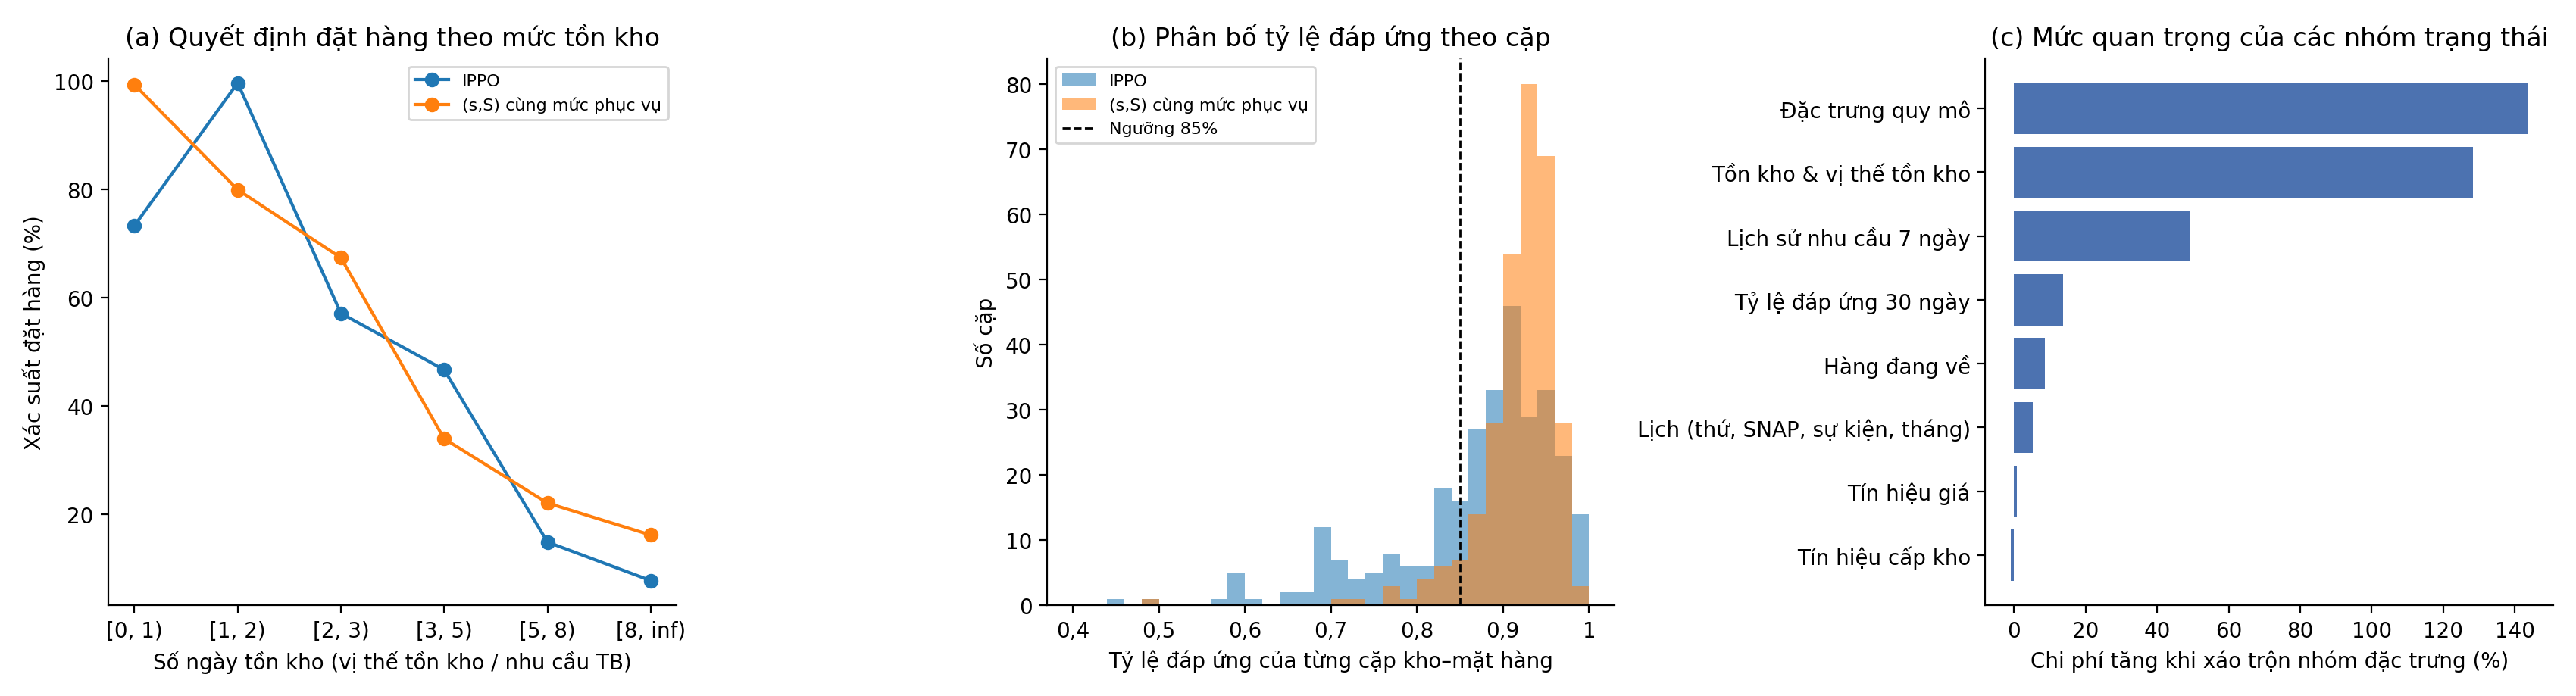
\includegraphics[width=\textwidth]{media/hinh_hanh_vi_chinh_sach.png}
    \caption{Hành vi của chính sách đã học}
    \label{fig:hanhVi}
\end{figure}

\subsubsection{Tính hợp lý về nghiệp vụ}

Hành vi đặt hàng của IPPO hợp lý về nghiệp vụ (Hình~\ref{fig:hanhVi}a, số ngày tồn kho bằng vị thế tồn kho chia cho nhu cầu trung bình):
\begin{itemize}
    \item Khi còn 1--2 ngày hàng, IPPO đặt hàng trong gần 100\% trường hợp. Xác suất đặt giảm gần đơn điệu, từ 57\% khi còn 2--3 ngày xuống 8\% khi còn trên 8 ngày.
    \item Tương quan hạng Spearman giữa số ngày tồn kho và mức đặt là $-$0,42, mạnh hơn $(s,S)$ cùng mức phục vụ ($-$0,17).
    \item IPPO chỉ dùng mức đặt lớn nhất ở 1,3\% số quyết định. Chi phí tràn kho chiếm 2,0\% tổng chi phí, so với 17,1\% của $(s,S)$ cùng mức phục vụ.
\end{itemize}

Có một điểm bất thường. Khi tồn kho dưới 1 ngày, IPPO chỉ đặt hàng trong 73\% trường hợp, thấp hơn nhóm 1--2 ngày. Các trường hợp này có thể tập trung ở cặp bán rất chậm, nhưng nhóm chưa kiểm tra.

Tác tử cũng thu hẹp lô hàng khi kho chật. Nhóm cố định mọi chiều quan sát của một cặp đại diện ở mức trung vị và chỉ cho mức sử dụng sức chứa tăng từ 20\% lên 95\%. Ngưỡng đặt hàng $s$ gần như không đổi, từ 1,348 lên 1,362 ngày nhu cầu, còn mức đặt tối đa $S$ giảm từ 5,65 xuống 5,09 ngày nhu cầu. Có 4 cặp ngừng đặt hàng hoàn toàn khi kho đạt 95\% sức chứa. Hành vi này do tác tử tự học qua phần thưởng, trong khi $(s, S)$ không quan sát trạng thái kho nên không làm được.

\subsubsection{Khai thác kẽ hở của phần thưởng}

Tác tử không dồn tỷ lệ đáp ứng sát ngưỡng, nhưng hạ mức phục vụ ở mặt hàng bán chậm (Hình~\ref{fig:hanhVi}b):
\begin{itemize}
    \item Chỉ 12,0\% số cặp nằm trong khoảng 85--88\%, nên tác tử không chỉ làm vừa đủ để tránh phạt.
    \item Có 28,7\% số cặp của IPPO dưới 85\%, với phân vị 10\% là 71,2\%. Với $(s,S)$ cùng mức phục vụ, con số này là 5,7\%, với phân vị 10\% là 87,9\%.
\end{itemize}

Tỷ lệ đáp ứng hệ thống 90,7\% của IPPO đạt được nhờ phục vụ rất tốt mặt hàng bán chạy, bù cho mặt hàng bán chậm. Tác tử tối ưu đúng hàm mục tiêu được giao, nhưng hàm mục tiêu đó chưa đòi hỏi mọi mặt hàng đều đạt mức phục vụ tối thiểu. Muốn mọi mặt hàng đạt mức phục vụ tối thiểu thì cần đặt ràng buộc ở cấp cặp, việc này nằm ngoài phạm vi đề tài.

\begin{table}[H]
    \centering
    \caption{Tầm quan trọng của các nhóm đặc trưng trạng thái}
    \label{tab:tamQuanTrong}
    \small
    \begin{tabular}{|l|c|c|c|}
        \hline
        Nhóm đặc trưng & Số chiều & Chi phí tăng & \tbc{Tỷ lệ đáp ứng}{thay đổi} \\
        \hline
        Đặc trưng quy mô $\log(1+\bar{D})$ & 1  & +143,6\% & $-$0,8 điểm \\ \hline
        Tồn kho và vị thế tồn kho           & 2  & +128,3\% & $-$28,9 điểm \\ \hline
        Lịch sử nhu cầu 7 ngày            & 7  & +49,3\% & $-$12,5 điểm \\ \hline
        Tỷ lệ đáp ứng cửa sổ 30 ngày      & 1  & +13,7\% & $-$0,5 điểm \\ \hline
        Hàng đang về                        & 3  & +8,6\%  & $-$0,5 điểm \\ \hline
        Lịch (thứ, SNAP, sự kiện, tháng)    & 27 & +5,3\%  & $-$0,2 điểm \\ \hline
        Tín hiệu giá (mức giảm giá)         & 1  & +0,8\%  & +0,1 điểm \\ \hline
        Tín hiệu cấp kho (mức đầy, tỷ trọng) & 2 & $-$0,8\%  & $-$0,3 điểm \\
        \hline
    \end{tabular}
    \ghichu{Mỗi nhóm đặc trưng được xáo trộn giữa các cặp ở mỗi bước. Riêng nhóm lịch được thay bằng lịch của một ngày ngẫu nhiên.}
\end{table}

\subsubsection{Biến dư thừa trong trạng thái}

Ba nhóm đặc trưng quyết định hành vi là đặc trưng quy mô, tồn kho và lịch sử nhu cầu. Mức tăng chi phí được đo bằng cách xáo trộn từng nhóm đặc trưng giữa các cặp, theo phương pháp tầm quan trọng hoán vị (\textit{permutation importance}):
\begin{itemize}
    \item Ba nhóm quan trọng nhất ứng đúng với các đại lượng mà chính sách tồn kho cổ điển cần là $\bar{D}$, vị thế tồn kho và $\sigma$.
    \item 27 chiều lịch chỉ đóng góp 5,3\% chi phí. Kết quả này phù hợp với việc IPPO yếu nhất ở mùa lễ.
    \item Tín hiệu giá và tín hiệu cấp kho gần như không đóng góp, vì xáo trộn chúng đổi chi phí dưới 1\%.
\end{itemize}

Tầm quan trọng hoán vị đo mức chính sách đã học dựa vào một đặc trưng, không đo hiệu năng khi huấn luyện lại không có đặc trưng đó. Với tín hiệu cấp kho, hai cách đo cho kết quả khác nhau (mục~\ref{subsec:ablationKhac}). Tín hiệu giá chưa có thí nghiệm loại trừ riêng.

\subsection{Đặc trưng lịch, giá và mùa lễ}
\label{subsec:lichGia}

Tác tử dùng rất ít tín hiệu lịch và giá, và mùa lễ là giai đoạn nó yếu nhất. Trong 44 chiều quan sát có 20 chiều lịch, 7 chiều thứ trong tuần, 1 tín hiệu giá và 16 chiều lịch sử, trạng thái. Tác tử chỉ thấy lịch của ngày hiện tại, không nhận dự báo nhu cầu tường minh. Ba phép đo cho kết quả nhất quán:
\begin{itemize}
    \item Xáo trộn nhóm lịch ở bước suy luận làm chi phí tăng 5,3\%, xáo trộn tín hiệu giá làm chi phí tăng dưới 1\% (Bảng~\ref{tab:tamQuanTrong}).
    \item Huấn luyện lại sau khi bỏ đặc trưng lịch, hoặc thêm đặc trưng sự kiện sắp tới, chỉ đổi chi phí trong phạm vi dao động giữa các hạt giống (Bảng~\ref{tab:ablationKhac}). Hai thí nghiệm này có một hạt giống và 1.000 tập, nên chưa đủ để kết luận.
    \item Ở mùa lễ, tỷ lệ đáp ứng của IPPO thấp nhất trong các giai đoạn. So với $(s,S)$, chi phí cao hơn 8,2\% nhưng khoảng tin cậy còn chứa 0 vì mùa lễ chỉ có 9 tuần. So với Newsvendor theo nhóm, chi phí cao hơn 10,1\% và khác biệt có ý nghĩa (Bảng~\ref{tab:ciGiaiDoan}).
\end{itemize}

Có hai giả thuyết cho kết quả này, cả hai đều chưa được kiểm chứng riêng. Thứ nhất, lịch sử nhu cầu 7 ngày đã chứa phần lớn tín hiệu mùa vụ ngắn hạn, nên đặc trưng lịch thêm được ít thông tin. Thứ hai, miền huấn luyện chỉ có khoảng ba mùa lễ, quá ít để mạng học được quy luật tăng cầu cuối năm từ các cờ nhị phân.

% [SO-MOI] So duoi day la so cua giao thuc cu; thay bang ket qua moi va them nguon cung chung, suc chua 3 va 8 ngay
\section{Câu hỏi 5: độ bền khi điều kiện vận hành thay đổi}
\label{sec:cau5}

Chính sách đã học bền với thay đổi sức chứa và thời gian giao hàng, nhưng kém khi nhu cầu giảm. Thí nghiệm chỉ thay đổi môi trường đánh giá (sức chứa kho, thời gian giao hàng, mức nhu cầu), còn mọi chính sách được giữ nguyên và không huấn luyện lại. Đây là đánh giá zero-shot (mục~\ref{subsec:dieuKien}):
\begin{itemize}
    \item Khi sức chứa và thời gian giao hàng thay đổi, IPPO vẫn rẻ hơn $(s,S)$ và EOQ ở mọi kịch bản, và ngang hoặc đắt hơn tối đa 4,6\% so với các chính sách theo nhóm.
    \item Khi nhu cầu tăng 20\%, IPPO rẻ hơn cả sáu chính sách đối chứng, từ 3,3\% đến 21,4\%.
    \item Khi nhu cầu giảm 20\%, IPPO đắt hơn năm trong sáu chính sách đối chứng, từ 4,2\% đến 8,7\%, vì tiếp tục giữ mức phục vụ cao (93,3\%) khi không cần thiết.
\end{itemize}

\begin{table}[H]
    \centering
    \caption{Độ bền khi điều kiện vận hành thay đổi}
    \label{tab:doBen}
    \footnotesize
    \setlength{\tabcolsep}{3pt}
    \begin{tabular}{|l|c|c|c|c|c|c|c|c|}
        \hline
        Kịch bản & IPPO & TLĐƯ & $(s,S)$ & $(s,S)$-N & EOQ & EOQ-N & NV & NV-N \\
        \hline
        Gốc                   & 2.051.839 & 90,7\% & $-1{,}9^{*}$ & +0,2 & $-18{,}0^{*}$ & $-1{,}1^{*}$ & $-0{,}5^{*}$ & $+1{,}4^{*}$ \\ \hline
        Sức chứa 4 ngày     & 2.191.998 & 89,0\% & $-3{,}0^{*}$ & $+0{,}7^{*}$ & $-23{,}1^{*}$ & $+0{,}5^{*}$ & $+1{,}0^{*}$ & $+4{,}6^{*}$ \\ \hline
        Sức chứa 6 ngày     & 2.032.325 & 91,1\% & $-$0,3 & $+1{,}1^{*}$ & $-14{,}3^{*}$ & $-0{,}9^{*}$ & $-0{,}3^{*}$ & $+1{,}0^{*}$ \\ \hline
        Giao hàng luôn 3 ngày & 2.156.456 & 88,1\% & $-3{,}1^{\sim}$ & $-2{,}0^{\sim}$ & $-20{,}4^{\sim}$ & $-10{,}5^{\sim}$ & $-0{,}0^{\sim}$ & $+0{,}2^{\sim}$ \\ \hline
        Giao hàng 2--3 ngày & 2.100.304 & 89,3\% & $-2{,}4^{*}$ & $-1{,}0^{*}$ & $-17{,}5^{*}$ & $-4{,}2^{*}$ & $-$0,1 & $+0{,}9^{*}$ \\ \hline
        Nhu cầu +20\%       & 2.351.070 & 87,8\% & $-7{,}7^{*}$ & $-5{,}4^{*}$ & $-21{,}4^{*}$ & $-5{,}7^{*}$ & $-5{,}6^{*}$ & $-3{,}3^{*}$ \\ \hline
        Nhu cầu $-$20\%       & 1.826.196 & 93,3\% & $+7{,}0^{*}$ & $+8{,}5^{*}$ & $-12{,}7^{*}$ & $+4{,}2^{*}$ & $+6{,}8^{*}$ & $+8{,}7^{*}$ \\
        \hline
    \end{tabular}
    \ghichu{Cột IPPO và TLĐƯ: chi phí và tỷ lệ đáp ứng của IPPO. Các cột còn lại: chênh lệch chi phí (\%) của IPPO so với từng chính sách đối chứng, âm là IPPO rẻ hơn. NV: Newsvendor. Hậu tố -N: phiên bản theo nhóm. Dấu $^{*}$: có ý nghĩa thống kê. Dấu $^{\sim}$: kịch bản tất định, không kiểm định được.}
\end{table}

Các chính sách đối chứng giữ tham số tinh chỉnh cho môi trường gốc. Vì vậy kết quả cho biết các chính sách đã có chịu đựng thay đổi thế nào, không so sánh các chính sách được chỉnh lại cho từng kịch bản.

\section{Độ tin cậy của kết luận}
\label{sec:doTinCay}

Các kết quả trên dựa trên một bộ đơn giá giả định và một cấu hình môi trường. Mục này kiểm tra kết luận có thay đổi khi các giả định đó thay đổi không.

\subsection{Độ nhạy của kết luận theo đơn giá chi phí}
\label{subsec:doNhay}

Kết luận ở cùng mức phục vụ giữ nguyên dấu khi đơn giá thay đổi, còn kết luận so trực tiếp phụ thuộc tỷ số $c_{th}/c_{lk}$. Để kiểm tra, các đại lượng vật lý của mỗi chính sách trên miền kiểm thử (đơn vị--ngày lưu kho, đơn vị thiếu hàng, số lần đặt, đơn vị tràn kho) được ghi lại. Tổng chi phí sau đó được tính lại trên 36 bộ đơn giá, với $c_{lk} \in \{0{,}5;\ 1;\ 2\}$, $c_{th} \in \{5;\ 10;\ 20;\ 40\}$ và $c_{dh} \in \{2;\ 5;\ 10\}$. Các chính sách không được huấn luyện hay tinh chỉnh lại, nên kết quả cho biết các chính sách đã có xếp hạng thế nào nếu chi phí được định giá khác đi.

\begin{table}[H]
    \centering
    \caption{Chênh lệch tổng chi phí của IPPO theo đơn giá ($c_{dh} = 5$)}
    \label{tab:doNhay}
    \small
    \setlength{\tabcolsep}{3pt}
    \begin{tabular}{|c|c|c|c|c|}
        \hline
        & $c_{th} = 5$ & $c_{th} = 10$ & $c_{th} = 20$ & $c_{th} = 40$ \\
        \hline
        $c_{lk} = 0{,}5$ & $-$1,7\% / $-$34,3\% & $-$8,3\% / $-$28,7\% & $-$15,5\% / $-$20,0\% & $-$21,8\% / $-$8,8\% \\ \hline
        $c_{lk} = 1$     & +3,6\% / $-$29,2\% & $-$1,9\% / $-$25,6\% & $-$9,0\% / $-$19,7\% & $-$16,3\% / $-$11,1\% \\ \hline
        $c_{lk} = 2$     & +7,6\% / $-$25,0\% & +3,8\% / $-$23,0\% & $-$2,0\% / $-$19,4\% & $-$9,3\% / $-$13,5\% \\
        \hline
    \end{tabular}
    \ghichu{Mỗi ô ghi chênh lệch so với $(s,S)$ trực tiếp / so với $(s,S)$ cùng mức phục vụ. Âm là IPPO rẻ hơn.}
\end{table}

Trên 36 bộ đơn giá:
\begin{itemize}
    \item Ở cùng mức phục vụ, IPPO rẻ hơn $(s,S)$ ở cả 36/36 bộ ($-$8,1\% đến $-$35,4\%) và rẻ hơn Newsvendor ở cả 36/36 bộ ($-$2,1\% đến $-$25,6\%).
    \item Ở phép so trực tiếp, IPPO rẻ hơn $(s,S)$ ở 26/36 bộ và Newsvendor ở 24/36 bộ. Chỉ EOQ bị IPPO vượt ở cả 36/36 bộ.
    \item Với các chính sách theo nhóm, IPPO chỉ rẻ hơn ở 18/36 bộ ($(s,S)$ theo nhóm), 21/36 bộ (Newsvendor theo nhóm) và 24/36 bộ (EOQ theo nhóm).
\end{itemize}

Khi thiếu hàng đắt so với lưu kho, IPPO rẻ hơn vì giữ mức phục vụ cao hơn. Khi lưu kho đắt và thiếu hàng rẻ, $(s,S)$ chấp nhận thiếu hàng nhiều hơn nên lại rẻ hơn. So với các chính sách theo nhóm, IPPO không có ưu thế chi phí ổn định ở phép so trực tiếp.

\section{Thảo luận và trả lời câu hỏi nghiên cứu}
\label{sec:thaoLuan}

% [SO-MOI] Viet lai theo ket qua moi: Cau hoi 1 da doi noi dung, them Cau hoi 4 va Cau hoi 5 (zero-shot)

Câu hỏi 1 hỏi PS-IPPO có rẻ hơn các chính sách đối chứng khi so sánh công bằng hay không. Câu trả lời phụ thuộc vào thông tin mà chính sách đối chứng có:
\begin{itemize}
    \item So với các chính sách cổ điển, IPPO rẻ hơn khi so ở cùng mức phục vụ: rẻ hơn 7,3--22,3\%, kể cả các phiên bản theo nhóm (mục~\ref{subsec:isoService}). Khi mỗi phương pháp dùng cấu hình tốt nhất của mình, IPPO có chi phí xấp xỉ nhưng mức phục vụ cao hơn 4--5 điểm phần trăm.
    \item So với chính sách biết sức chứa, IPPO rẻ hơn (mục~\ref{subsec:soSanhThongTin}).
    \item So với chính sách dùng dự báo, IPPO đắt hơn, kể cả khi hai bên có mức phục vụ gần nhau. Vì vậy đề tài chưa thể kết luận học tăng cường thay được dự báo rồi tối ưu.
    \item Dùng IPPO cho nhóm nhu cầu cao và dự báo cho các nhóm còn lại rẻ hơn IPPO 3,2\%, nhưng vẫn đắt hơn chính sách dự báo 1,0\% (mục~\ref{subsec:ketHop}).
    \item Ưu thế không tuyệt đối. Khi nhu cầu ổn định hoặc vào mùa lễ, chính sách tinh chỉnh theo nhóm rẻ hơn hoặc ngang IPPO. Ưu thế của IPPO tập trung ở độ bền mức phục vụ khi nhu cầu biến động, ở ngày sự kiện, cuối tuần và khi có sốc cầu (mục~\ref{subsec:hanChe}).
\end{itemize}

Câu hỏi 2 là chia sẻ tham số có giữ được hiệu năng trên các cặp có quy mô khác nhau hay không. Câu trả lời là có ở nhóm nhu cầu trung bình và cao:
\begin{itemize}
    \item Ở hai nhóm này, IPPO tốt hơn $(s, S)$ cả về chi phí lẫn mức phục vụ (mục~\ref{subsec:tongQuatHoa}).
    \item Ở nhóm bán chậm, IPPO hạ mức phục vụ vì đó là lựa chọn rẻ hơn theo hàm mục tiêu cấp hệ thống.
    \item Chính sách học được áp dụng được cho mặt hàng chưa gặp khi huấn luyện mà không suy giảm.
\end{itemize}

Câu hỏi 3 là thiết kế phần thưởng ảnh hưởng thế nào tới độ ổn định và hiệu năng. Phần thưởng phân rã cục bộ có chuẩn hóa theo cặp là cần thiết (mục~\ref{subsec:ablationReward}):
\begin{itemize}
    \item Thay bằng phần thưởng toàn cục hoặc bỏ chuẩn hóa theo cặp đều làm chi phí tăng hơn gấp ba ở cả ba hạt giống.
    \item Phương sai giải thích được cao của Critic trong hai biến thể cho thấy nguyên nhân là vài cặp nhu cầu lớn chi phối tín hiệu học.
\end{itemize}

Câu hỏi 5 là mô hình đã huấn luyện còn bền không khi điều kiện vận hành thay đổi. Với thay đổi sức chứa và thời gian giao hàng, IPPO vẫn rẻ hơn $(s,S)$ và EOQ. Khi nhu cầu giảm, IPPO đắt hơn vì tiếp tục giữ mức phục vụ cao (mục~\ref{sec:cau5}). Đây là đánh giá không huấn luyện lại, nên đề tài chưa kết luận được mô hình sẽ học gì nếu được huấn luyện trong từng điều kiện.
% [SO-MOI] Bo sung ket luan nguon cung chung va suc chua 3, 8 ngay khi co ket qua

Ngoài các câu hỏi trên, kết quả còn cho thấy vai trò của ràng buộc sức chứa. Khi sức chứa đủ rộng, bài toán suy biến thành 300 bài toán độc lập (mục~\ref{subsec:kichBan}). Chính sức chứa dùng chung tạo nên bản chất đa tác tử của bài toán. Đây cũng là yếu tố mà hai công trình gần nhất chưa mô hình hóa: Zhu và Wu \cite{zhu2026spatiotemporal} giả định nguồn cung không giới hạn, còn Nam và cộng sự \cite{jeong2026alca} chỉ xét một kho.

\FloatBarrier
IPPO rẻ hơn mọi chính sách cổ điển khi so ở cùng mức phục vụ, nhưng chưa vượt được chính sách dùng dự báo. Hạn chế chính là chưa khai thác được thông tin về nhu cầu tương lai và mức phục vụ chưa đồng đều ở mặt hàng bán chậm. Chương~\ref{chap:chapter5} tổng kết các kết quả này và đề xuất hướng phát triển.

    \chapter{KẾT LUẬN VÀ HƯỚNG PHÁT TRIỂN}
\label{chap:chapter5}

\section{Kết quả đạt được}
\label{sec:tongKet}

Đề tài đã hoàn thành cả sáu mục tiêu đặt ra ở Chương~\ref{chap:tongquan}. Mỗi mục tiêu được đặt cạnh kết quả tương ứng để thấy mức độ hoàn thành.

\begin{table}[H]
    \centering
    \caption{Đối chiếu mục tiêu và kết quả}
    \label{tab:doiChieuMucTieu}
    \small
    \begin{tabular}{|c|>{\raggedright\arraybackslash}p{5.0cm}|>{\raggedright\arraybackslash}p{8.2cm}|}
        \hline
        STT & Mục tiêu & Kết quả \\
        \hline
        1 & Môi trường mô phỏng nhiều kho, nhiều mặt hàng theo chuẩn Gymnasium & Môi trường 10 kho, 30 mặt hàng (300 cặp) với nhu cầu M5, thời gian giao hàng 1--3 ngày, sức chứa riêng từng kho, bốn thành phần chi phí và hình phạt mức phục vụ tách khỏi chi phí vận hành \\ \hline
        2 & Phần thưởng phân rã cục bộ kèm phạt mức phục vụ & Phần thưởng theo từng cặp, chuẩn hóa theo cặp, phạt mức phục vụ trên cửa sổ trượt 30 ngày. Thí nghiệm loại trừ xác nhận thiết kế này là cần thiết \\ \hline
        3 & Cài đặt và huấn luyện IPPO chia sẻ tham số & 300 tác tử dùng chung một mạng, huấn luyện 10.000 tập với 3 hạt giống, hội tụ ổn định ở cả 3 hạt giống. Biến thể kết hợp dự báo cũng được huấn luyện với 3 hạt giống \\ \hline
        4 & Đánh giá so với các chính sách đối chứng & So sánh trực tiếp và ở cùng mức phục vụ với chính sách cổ điển, chính sách biết sức chứa và chính sách dự báo rồi tối ưu, có kiểm định thống kê, phân tích theo giai đoạn nhu cầu và độ nhạy đơn giá \\ \hline
        5 & Độ bền của mô hình khi điều kiện vận hành thay đổi & Đánh giá mô hình chính đã huấn luyện, không huấn luyện lại, khi đổi sức chứa, thời gian giao hàng, mức nhu cầu và khi có nguồn cung chung giữa các kho \\ \hline
        6 & Ứng dụng mô phỏng & Ứng dụng nạp mô hình đã huấn luyện, chạy trên miền kiểm thử, hiển thị kết quả, diễn biến từng cặp, kịch bản tăng cầu và phiếu đề nghị đặt hàng \\
        \hline
    \end{tabular}
\end{table}

\section{Kết luận}
\label{subsec:traLoiCauHoi}

Trên mạng lưới nhiều kho có sức chứa dùng chung, học tăng cường đa tác tử với chia sẻ tham số rẻ hơn các chính sách cổ điển khi so ở cùng mức phục vụ. Khi được kết hợp với dự báo nhu cầu, mô hình đạt chi phí của chính sách dự báo rồi tối ưu và rẻ hơn mọi chính sách cổ điển.

Với Câu hỏi 1, ở cùng mức phục vụ IPPO rẻ hơn các chính sách cổ điển từ 7,3\% đến 16,3\% ở cả ba hạt giống, kể cả các phiên bản theo nhóm và phiên bản biết sức chứa, và rẻ hơn EOQ trên 22\%. Kết luận này không đổi trên 36 bộ đơn giá và ở mọi giai đoạn nhu cầu. Khi mỗi phương pháp dùng cấu hình tốt nhất của mình, IPPO rẻ hơn $(s, S)$ và EOQ ở cả ba hạt giống và giữ mức phục vụ cao hơn 4--5 điểm phần trăm. Ưu thế của IPPO tập trung ở ngày có sự kiện, cuối tuần và khi có sốc cầu. Khi nhu cầu ổn định, chính sách cổ điển tinh chỉnh theo nhóm vẫn cạnh tranh được.

Với Câu hỏi 2, một bộ trọng số dùng chung điều khiển được 300 cặp có nhu cầu chênh nhau hơn ba bậc độ lớn. Ở nhóm nhu cầu trung bình và cao, IPPO tốt hơn $(s, S)$ cả về chi phí lẫn mức phục vụ. Chính sách học được cũng áp dụng được cho mặt hàng chưa gặp khi huấn luyện mà không suy giảm. Ở nhóm bán chậm, IPPO hạ mức phục vụ vì đó là lựa chọn rẻ hơn theo hàm mục tiêu cấp hệ thống.

Với Câu hỏi 3, phần thưởng phân rã cục bộ có chuẩn hóa theo cặp là cần thiết. Thay bằng phần thưởng toàn cục hoặc bỏ chuẩn hóa đều làm chi phí tăng hơn gấp ba ở cả 3 hạt giống.

Với Câu hỏi 4, kết hợp dự báo giảm chi phí của PS-IPPO 7,7\% so với mô hình chính. Khi tác tử chọn hệ số an toàn trên nền dự báo LightGBM, PS-IPPO rẻ hơn mọi chính sách cổ điển từ 6,2\% đến 24,1\% và ngang Newsvendor dự báo ở cả ba hạt giống. Khi so ở cùng mức phục vụ, mô hình vẫn rẻ hơn chính sách cổ điển từ 6,0\% đến 17,8\%. Phần lớn lợi thế này đến từ dự báo. Học tăng cường cho phép tích hợp dự báo mà không đổi môi trường hay thuật toán, và tự chọn mức an toàn thay cho việc quét lưới tham số.

Với Câu hỏi 5, mô hình đã huấn luyện vẫn rẻ hơn $(s, S)$ và EOQ khi sức chứa và thời gian giao hàng thay đổi, và rẻ hơn mọi chính sách đối chứng khi nhu cầu tăng 20\%. Khi các kho dùng chung một nguồn cung có giới hạn, mô hình rẻ hơn mọi chính sách cổ điển từ 1,1\% đến 22,4\%, dù các chính sách đối chứng đã được tinh chỉnh lại cho môi trường mới. Nguồn cung càng chặt thì lợi thế càng lớn. Khi nhu cầu giảm, mô hình đắt hơn phần lớn chính sách đối chứng vì tiếp tục giữ mức phục vụ cao. Nhóm không huấn luyện lại mô hình dưới các điều kiện này, nên kết luận chỉ nói về độ bền của mô hình đã có.

Từ các kết quả trên, đề tài có bốn đóng góp. Thứ nhất, đề tài xây dựng một môi trường mô phỏng tồn kho 10 kho, 30 mặt hàng hiệu chỉnh từ dữ liệu bán lẻ thực tế. Trong môi trường này, sức chứa dùng chung là yếu tố tạo nên bản chất đa tác tử của bài toán. Thứ hai, đề tài thiết kế và kiểm chứng phần thưởng phân rã cục bộ có chuẩn hóa theo cặp, giúp 300 tác tử với quy mô rất khác nhau học ổn định trên cùng một mạng. Thứ ba, đề tài cho thấy PS-IPPO rẻ hơn các chính sách cổ điển ở cùng mức phục vụ và tự học được cách thu hẹp lô hàng khi kho chật. Khi kết hợp với dự báo nhu cầu, mô hình đạt chi phí của chính sách dự báo tốt nhất. Thứ tư, đề tài áp dụng một giao thức đánh giá có kiểm soát. Giao thức gồm so sánh ở cùng mức phục vụ, chính sách đối chứng chia theo loại thông tin, nhiều hạt giống, kiểm định theo cặp và phân tích theo giai đoạn nhu cầu. Giao thức này giúp kết luận không bị sai lệch khi các phương pháp nằm ở những điểm khác nhau trên đường đánh đổi giữa chi phí và mức phục vụ.

Về ứng dụng, kết quả gợi ý doanh nghiệp nên đầu tư vào dự báo nhu cầu trước, vì đây là phần mang lại lợi ích lớn nhất. Khi đã có dự báo, học tăng cường có thể đảm nhận việc chọn mức an toàn cho từng mặt hàng có tính tới sức chứa kho, thay cho việc chỉnh tay tham số. Chính sách cổ điển vẫn đủ tốt cho nhóm hàng có nhu cầu ổn định. Ứng dụng mô phỏng của đề tài cho phép người quản lý xem trước tác động của chính sách trước khi áp dụng.

\section{Hạn chế}
\label{sec:hanChe}

Các hạn chế dưới đây được xếp theo mức ảnh hưởng tới kết luận. Hạn chế ảnh hưởng nhiều nhất là phần đóng góp riêng của học tăng cường khi đã có dự báo còn nhỏ. Biến thể kết hợp dự báo đạt chi phí ngang Newsvendor dự báo nhưng chưa rẻ hơn rõ rệt, và mô hình được chọn nằm ở giai đoạn đầu của quá trình huấn luyện. Mô hình chính không nhận dự báo nên đắt hơn chính sách dự báo. Vì vậy đề tài chưa thể kết luận học tăng cường thay được dự báo rồi tối ưu, mà chỉ cho thấy hai cách tiếp cận kết hợp được với nhau.

Hạn chế thứ hai là mức phục vụ không đồng đều giữa các mặt hàng. Dù đã dùng hình phạt chuẩn hóa, 28,7\% số cặp vẫn có tỷ lệ đáp ứng dưới 85\%, tập trung ở nhóm bán chậm. Mục tiêu mức phục vụ chỉ được đáp ứng ở cấp hệ thống. Hạn chế này ảnh hưởng tới việc áp dụng trong thực tế, khi doanh nghiệp cần cam kết mức phục vụ cho từng mặt hàng.

Hạn chế thứ ba là số hạt giống của từng phân tích. Kết quả chính được kiểm chứng với 3 hạt giống, nên khoảng tin cậy giữa các hạt giống còn rộng. Các phân tích sâu chỉ dùng mô hình của một hạt giống. Phần lớn thí nghiệm loại trừ chỉ có một hạt giống và 1.000 tập. Do đó các kết luận từ những thí nghiệm này, nhất là vai trò của tín hiệu cấp kho, mới ở mức gợi ý.

Hạn chế thứ tư là đề tài chưa so sánh với phối hợp tường minh. Các tác tử chỉ phối hợp gián tiếp qua tín hiệu sức chứa. Vì vậy chưa định lượng được giá trị mà một Critic tập trung theo hướng CTDE \parencite{yu2022mappo} có thể mang lại. Câu hỏi này đáng quan tâm vì Zhu và Wu \cite{zhu2026spatiotemporal} báo cáo hiệu năng giảm đáng kể khi bỏ cơ chế phối hợp trong khung của họ.

Hạn chế thứ năm thuộc về phạm vi mô hình. Mô hình chính gồm các kho song song. Nguồn cung chung giữa các kho chỉ được xét ở phần đánh giá không huấn luyện lại, với một cách chia theo tỷ lệ. Đề tài không huấn luyện lại mô hình dưới nguồn cung chung hay sức chứa khác, không khảo sát mức chia sẻ tham số, quy mô trên 300 tác tử và độ nhạy siêu tham số. Đề tài chưa xét cấu trúc đa cấp \parencite{clark1960} hay điều chuyển hàng giữa các kho. Không gian hành động chỉ có 6 mức đặt hàng. Mô hình chính dùng trực tiếp lịch sử nhu cầu, còn dự báo chỉ được tích hợp ở một biến thể. Các đặc trưng lịch và giá gần như không được khai thác, và IPPO yếu nhất ở mùa lễ.

Hạn chế cuối cùng thuộc về dữ liệu và môi trường đánh giá. Dữ liệu M5 là dữ liệu bán lẻ của Walmart tại Hoa Kỳ. M5 ghi doanh số chứ không ghi nhu cầu thật và không đánh dấu ngày hết hàng, nên nhu cầu đầu vào có thể thấp hơn thực tế ở mức chưa đo được. Mười kho của đề tài là mười cửa hàng của M5 được xem như các điểm lưu trữ độc lập, và sức chứa là giả định. Đơn giá chi phí cũng là giả định của đề tài, và phân tích độ nhạy giữ nguyên chính sách đã học. Mô hình mới được kiểm chứng trên môi trường mô phỏng, chưa trên dữ liệu vận hành trực tiếp. Mô hình học từ dữ liệu nên khi áp dụng cho Việt Nam cần huấn luyện lại trên dữ liệu bán hàng trong nước và thay vector lịch Hoa Kỳ bằng lịch lễ Việt Nam. Kiến trúc mô hình và quy trình huấn luyện có thể giữ nguyên.

\section{Hướng phát triển}
\label{sec:huongPhatTrien}

Các hướng dưới đây cần dữ liệu hoặc hệ thống thật, hoặc đổi sang một lớp bài toán khác, nên nằm ngoài những gì đề tài làm được với dữ liệu M5. Với mỗi hướng, nhóm ghi lại lý do chưa thực hiện và phần đề tài đã chuẩn bị sẵn để có thể làm tiếp.

\begin{longtable}{|c|>{\raggedright\arraybackslash}p{3.9cm}|>{\raggedright\arraybackslash}p{5.1cm}|>{\raggedright\arraybackslash}p{3.8cm}|}
    \caption{Hướng phát triển và phần đề tài đã chuẩn bị}
    \label{tab:huongPhatTrien} \\
    \hline
    STT & Hướng phát triển & Lý do chưa thực hiện & Phần đã chuẩn bị \\
    \hline
    \endfirsthead
    \hline
    STT & Hướng phát triển & Lý do chưa thực hiện & Phần đã chuẩn bị \\
    \hline
    \endhead
    1 & Triển khai trên hệ thống quản lý kho thật và thử nghiệm đối chứng tại doanh nghiệp & Cần quyền truy cập hệ thống và dữ liệu vận hành & Phiếu mua sắm, bản thử nghiệm Model Context Protocol \\ \hline
    2 & Dữ liệu Việt Nam và hiệu chỉnh chi phí thật & Không có dữ liệu. M5 không có giá vốn, chi phí đặt hàng, chi phí lưu kho & Độ nhạy theo 36 bộ đơn giá. Giữ nguyên kiến trúc, thay vector lịch \\ \hline
    3 & Khôi phục nhu cầu bị cắt do hết hàng & Cần cờ hết hàng hoặc tồn kho theo ngày, M5 không có & Kịch bản nhu cầu tăng 20\%, nêu rõ ở hạn chế \\ \hline
    4 & Chuyển hàng ngang giữa kho và mạng nhiều tầng có kho trung tâm & Đổi lớp bài toán. Cần chi phí, thời gian chuyển hàng mà M5 không có, và phải thiết kế lại môi trường, chính sách đối chứng và phép so sánh & Đánh giá không huấn luyện lại với nguồn cung chung giữa các kho \\ \hline
    5 & Học tăng cường ngoại tuyến từ nhật ký quyết định & Cần nhật ký quyết định và kết quả thật & Ứng dụng mô phỏng ghi lại quyết định theo ngày \\ \hline
    6 & Bảo đảm hình thức cho ràng buộc mức phục vụ & Cần khung lý thuyết có chặn xác suất vi phạm. Đề tài chỉ xử lý ràng buộc mềm & Khảo sát thực nghiệm hệ số phạt mức phục vụ \\ \hline
    7 & Tương tác với nhà cung cấp: giá động, số lượng tối thiểu, hợp đồng, nhiều nguồn cung & Sản phẩm của đề tài dừng ở phiếu gửi phòng mua hàng. Thiếu dữ liệu & Ghi chú phạm vi trên trang phiếu \\ \hline
    8 & Nghiên cứu người dùng với nhân viên mua hàng & Cần người dùng thật & Luồng duyệt phiếu trong ứng dụng \\ \hline
    9 & Critic tập trung trên toàn mạng 300 cặp & Các cặp chỉ liên kết qua sức chứa trong từng kho. Đầu vào khoảng 13.200 chiều với một quỹ đạo mỗi bước làm giảm hiệu quả mẫu & Tín hiệu cấp kho trong quan sát \\ \hline
    10 & Huấn luyện lại dưới nguồn cung chung hoặc sức chứa khác, mở rộng quy mô, khảo sát mức chia sẻ tham số và độ nhạy siêu tham số & Mỗi nội dung cần huấn luyện riêng, nằm ngoài phạm vi của đề tài & Cấu hình môi trường và đánh giá không huấn luyện lại \\
    \hline
\end{longtable}

    % Tiêu đề "TÀI LIỆU THAM KHẢO" căn giữa, có trong mục lục
    \printbibheading[heading=bibcenter, title={TÀI LIỆU THAM KHẢO}]

    % In theo nhóm chủ đề (khai báo trong preamble.tex), đánh số liên tục [1], [2], ...
    \printbibliography[category=tonkho, heading=subbib, title={Lý thuyết tồn kho}]
    \printbibliography[category=rl, heading=subbib, title={Học tăng cường}]
    \printbibliography[category=marl, heading=subbib, title={Học tăng cường đa tác tử}]
    \printbibliography[category=rltonkho, heading=subbib, title={Học tăng cường cho quản lý tồn kho}]
    \printbibliography[category=dubao, heading=subbib, title={Dự báo nhu cầu và bộ dữ liệu M5}]
    \printbibliography[category=danhgia, heading=subbib, title={Môi trường mô phỏng và đánh giá}]

\end{document}